\documentclass[a4paper,12pt]{article}
%\documentclass{Configuration_Files/Template}

%------------------------------------------------------------------------------
%	REQUIRED PACKAGES AND  CONFIGURATIONS
%------------------------------------------------------------------------------

% CONFIGURATIONS
\usepackage{parskip} % For paragraph layout
\usepackage{setspace} % For using single or double spacing
\usepackage{emptypage} % To insert empty pages
\usepackage{multicol} % To write in multiple columns (executive summary)
\setlength\columnsep{15pt} % Column separation in executive summary
\setlength\parindent{0pt} % Indentation
\raggedbottom  

% PACKAGES FOR TITLES
\usepackage{titlesec}
% \titlespacing{\section}{left spacing}{before spacing}{after spacing}
\titlespacing{\section}{0pt}{3.3ex}{2ex}
\titlespacing{\subsection}{0pt}{3.3ex}{1.65ex}
\titlespacing{\subsubsection}{0pt}{3.3ex}{1ex}
\usepackage{color}

% PACKAGES FOR LANGUAGE AND FONT
\usepackage[english]{babel} % The document is in English  
\usepackage[utf8]{inputenc} % UTF8 encoding
\usepackage[T1]{fontenc} % Font encoding
\usepackage[11pt]{moresize} % Big fonts

% PACKAGES FOR IMAGES
\usepackage{graphicx}
\usepackage{transparent} % Enables transparent images
\usepackage{eso-pic} % For the background picture on the title 
\usepackage{rotating}
\usepackage{subfig} % Numbered and caption subfigures using \subfloat.
\usepackage{tikz} % A package for high-quality hand-made figures.
\usetikzlibrary{}
\graphicspath{{./Images/}} % Directory of the images
\usepackage{caption} % Coloured captions
\usepackage{amsthm,thmtools,xcolor} % Coloured "Theorem"
\usepackage{float}

% STANDARD MATH PACKAGES
\usepackage{amsmath}
\usepackage{amsthm}
\usepackage{amssymb}
\usepackage{amsfonts}
\usepackage{bm}
\usepackage[overload]{empheq} % For braced-style systems of equations.
\usepackage{fix-cm} % To override original LaTeX restrictions on sizes

% PACKAGES FOR TABLES
\usepackage{tabularx}
\usepackage{longtable} % Tables that can span several pages
\usepackage{colortbl}
\usepackage{multicol}
\newcolumntype{C}[1]{>{\centering\arraybackslash}m{#1}} % Centered column type
\setlength\columnsep{15pt}

% PACKAGES FOR ALGORITHMS (PSEUDO-CODE)
\usepackage{algorithm}
\usepackage{algorithmic}

% PACKAGES FOR REFERENCES & BIBLIOGRAPHY
\usepackage[colorlinks=true,linkcolor=black,anchorcolor=black,citecolor=black,filecolor=black,menucolor=black,runcolor=black,urlcolor=black]{hyperref} % Adds clickable links at references
\usepackage{cleveref}
\usepackage[square, numbers, sort&compress]{natbib} % Square brackets, citing references with numbers, citations sorted by appearance in the text and compressed
\bibliographystyle{abbrvnat} % You may use a different style adapted to your field

% OTHER PACKAGES
\usepackage{pdfpages} % To include a pdf file
\usepackage{afterpage}
\usepackage{lipsum} % DUMMY PACKAGE
\usepackage{fancyhdr} % For the headers
\fancyhf{}

%----------------------------------------------------------------------------
%	NEW COMMANDS DEFINED
%----------------------------------------------------------------------------

% EXAMPLES OF NEW COMMANDS
\newcommand{\bea}{\begin{eqnarray}} % Shortcut for equation arrays
\newcommand{\eea}{\end{eqnarray}}
\newcommand{\e}[1]{\times 10^{#1}}  % Powers of 10 notation

%----------------------------------------------------------------------------
%	ADD YOUR PACKAGES (be careful of package interaction)
%----------------------------------------------------------------------------

\usepackage{geometry}
\usepackage{tabularx}
\usepackage{booktabs,xltabular}

%----------------------------------------------------------------------------
%	ADD YOUR DEFINITIONS AND COMMANDS (be careful of existing commands)
%----------------------------------------------------------------------------

% Set uniform margins
\geometry{
  left=0.8in,
  right=0.8in,
  top=1in,
  bottom=1in,
  includehead,
  includefoot
}

\begin{document}
\title{Students\&Companies Design Document} % Title Page
\author{Alessandro Salvatore, Erdal Yalçın, Leonardo Ratti}
\date{Academic Year: 2024-25}
\maketitle


\newpage
\tableofcontents
\section{Introduction}
\subsection{Purpose}
This document contains the design description of the Students\&Company system. It includes
the architectural design, the user interface design and the descrpition of the operations
that the system will perform. It also show how the requirements and use cases detailed
in the RASD document are satisfied by the design of the system. \\ \newline 
This document is intended to be read by the developers of the system, the testers and the
project managers. It is also intended to be used as a reference for the future maintenance
of the system.
\subsection{Scope}
The Students\&Company system is a web application that allows companies to advertise internship opportunities
for university students. A recommendation system is used for enhancing the matching possibilities between the two parties.
The system provides also suggestions for students and companies to increase their chances to get matched by the recommendation system. \\ \newline
A more detailed description of the system can be found in the RASD document, whilist in
this document is provided a detailed description of the design of the system to implement
the requirements and use cases described in the RASD document.
\subsubsection{Definitions}
    \begin{itemize}
        \item \textbf{User}: with User we refer to an active individual that can be either a Student, a Comapny or a University.
        \item \textbf{Advertise}: An Internship is advertised only if it has been posted and its application deadline is not yet expired.
        \item \textbf{Recommendation}: It's a platform feature that starts a matching between a company and a student. If both parties accept the recommendation, the student is taken for the selection process
        \item \textbf{Applying}: a student applies for an internship if he/she manually searches for it and applies for it and the internship was not recommended to him/her.
        \item \textbf{Accepting}: The act of students or companies, who got recommended to each other, to confirm their interest.
        \item \textbf{Contact}: The mutual acceptance of recommendation between student and company on the same internship.
        \item \textbf{Selection}: It's the process that starts after the expiration date of applying for the internship. The company interviews every accepted student and picks the best one(s) for their needs.
        \item \textbf{Selected student}: He is the student who has been chosen for the internship by the company.
        \item \textbf{Candidate}: he is a Student that has passed to the selection phase of an internship.
        \item \textbf{Feedback}: Consists of two separate moments.
        The first round of feedback is when the users likes/dislikes the recommendation given by the system. The second type of feedback is submitted after the end of the internship, where students and companies rate the experience through a 5 star review form.
        \item \textbf{Comment}: Is anything written in the dedicated Comments section. Serves the student or the company currently engaged, to highlight something about the experience with each other. If that's a complaint from either, the University of the student will manage the situation.
        \item \textbf{Complaint}: It's a specific type of Observation, where the University of the student can manage the situation between the parties.
        \item \textbf{Observation}: It's a type of comment that is not a complaint. It could just report some good or neutral facts about the experience.
    \end{itemize}
\subsubsection{Acronyms}
    \begin{itemize}
        \item S\&C: "Students\&Companies", the name of the platform
    \end{itemize}
\subsubsection{Abbreviations}
    \begin{itemize}
        \item \textbf{Wn}: n-th World Phenomena
        \item \textbf{Sn}: n-th Shared Phenomena
        \item \textbf{Gn}: n-th Goal
        \item \textbf{Dn}: n-th Domain Assumption
        \item \textbf{Rn}: n-th Requirement
        \item \textbf{Cn}: n-th Component
    \end{itemize}
\subsection{Revision History}
\noindent
\begin{tabularx}{\textwidth}{llX}
    \toprule
    Revised on & Version & Description \\
    \midrule
    07-Jan-2025 & 1.0 & Initial Release of the document \\
    \bottomrule
\end{tabularx}
\subsection{Reference Documents}
    \begin{itemize}
        \item The specification document of the project: \textbf{Assignment RDD AY 2024-2025}
        \item The \textbf{RASD} document of the project

    \end{itemize}
\subsection{Document Structure}
The document is divided into 6 sections:

\begin{itemize}
    \item \textbf{Introduction}: provides a brief description of the purpose and the scope of the system. Moreover, it contains the definitions, acronyms, and abbreviations used in the document and the reference documents.
    
    \item \textbf{Architectural Design}: this section provides a description of the architecture of the system, including the components and the interfaces between them. It also includes the runtime view of the most important operations of the system, the deployment view, and the architectural styles and patterns used in the system.
    
    \item \textbf{User Interface Design}: includes the mockups of the user interface of the system.
    
    \item \textbf{Requirements Traceability}: this section shows how the requirements described in the RASD document are satisfied by the design of the system.
    
    \item \textbf{Implementation, Integration and Test Plan}: this includes the step-by-step plan for the implementation and testing of the system.
    
    \item \textbf{Effort Spent}: this section highlights the effort spent by each member of the group to redact this document.
\end{itemize}
\newpage

\section{Overall Description}
\subsection{Overview: High-level Components and Interaction}
The following diagram is designed to clearly demonstrate the high-level components required by the system and the relationships between them.

 The Presentation Layer interacts directly with users and is responsible for managing the front-end side. This layer provides the user interface and collaborates with the Load Balancer and Web Server to optimize system performance and functionality. User interactions within the interface are forwarded from the Presentation Layer to the back-end, enabling additional processing and functionality. Furthermore, to enhance the system’s security and mitigate potential threats from external networks, a Firewall component is incorporated into the architecture. The Business Logic Layer processes incoming requests from the Presentation Layer and facilitates access to the core system functionalities, such as internship applications and recommendation mechanisms, through the use of APIs and Services. In summary, the Business Logic Layer, which houses the Application Server designed in accordance with RESTful standards, ensures the seamless transfer of operations to the Data Layer, thus ensuring the system operates in an efficient, secure, and effective manner.
\begin{figure}[H]
\centering
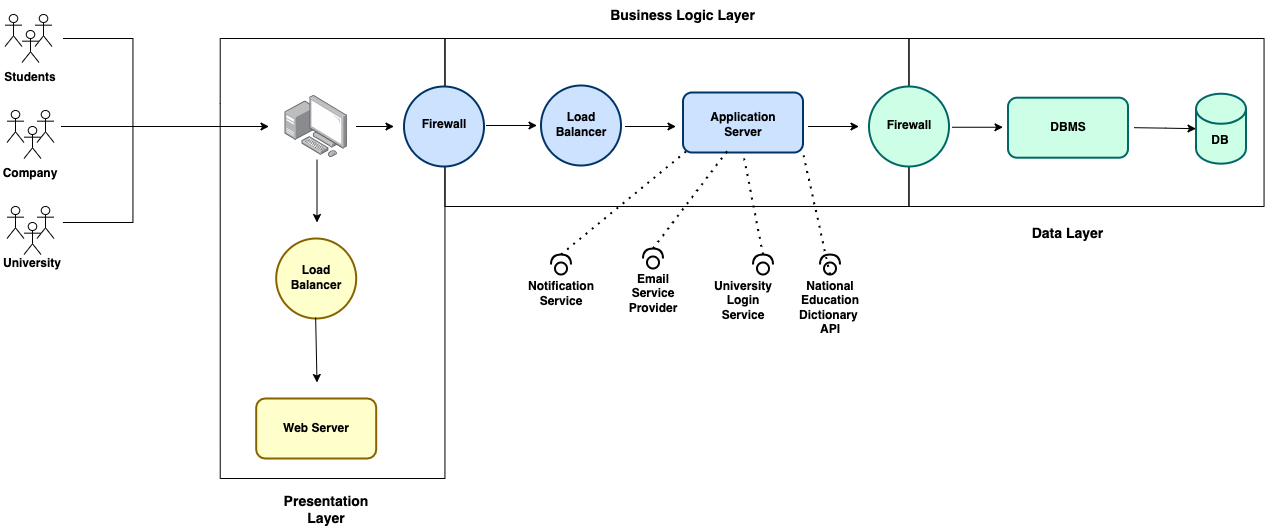
\includegraphics[scale = 0.40]{DD_figures/SingleDiagrams/overviewDiagram.png}
\end{figure}

\newpage
\subsection{Component View}
In this section we show the components and their relationships. The following
sections will explain the interaction between interfaces and details on each method of interfaces.
\begin{figure}[H]
\centering
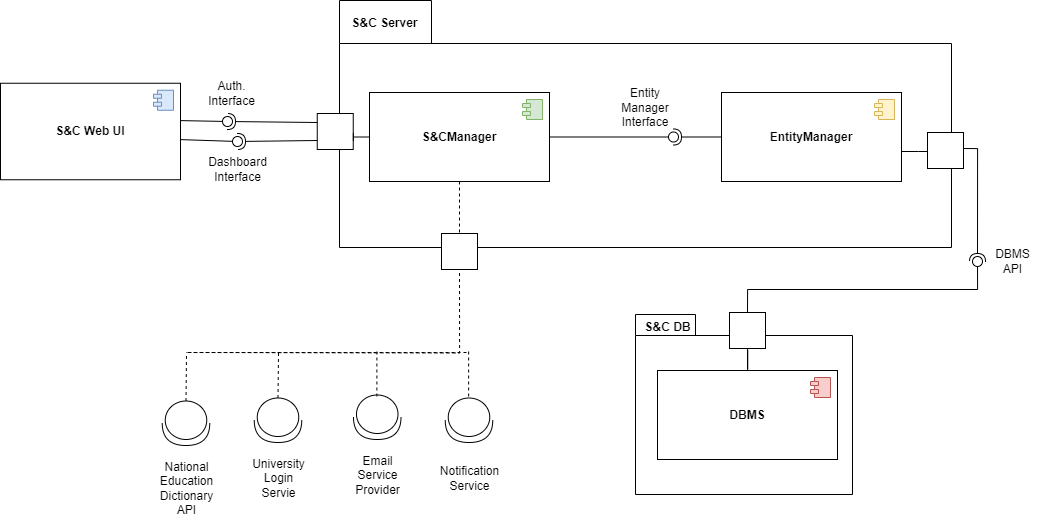
\includegraphics[scale = 0.50]{DD_figures/GeneralComponentDiagram.drawio.png}\\
\caption{Component Diagram of the Student\&Companies System}
\end{figure}

\subsubsection{DB Manager}
This component is responsible for communication with a Database Management System (DBMS).
It follows the Adapter design pattern, allowing other components to interact with the DBMS
without needing to write any SQL code themselves.
\subsubsection{S\&C-SP}
The S\&C-SP subsystem implements S\&C's logic. It provides all the system's features, including the recommendation system.
\begin{sidewaysfigure}% Use sidewaysfigure instead of figure
\centering
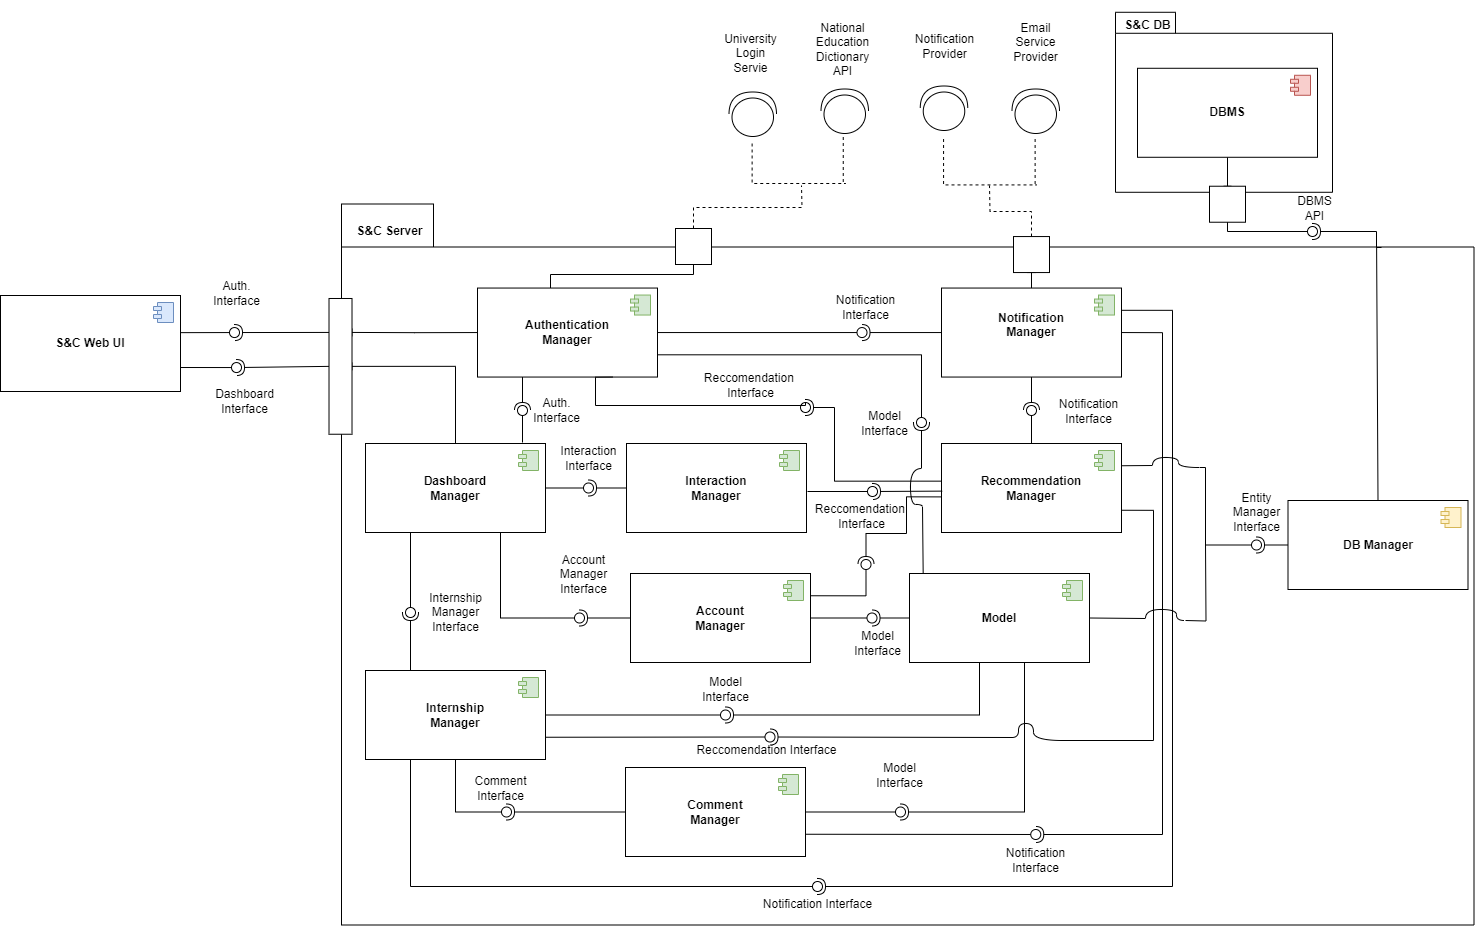
\includegraphics[scale=0.50]{DD_figures/ComponentDiagram2-S&C.drawio.png}\\
\caption{Component Diagram of the S\&C-SP subsystem}
\end{sidewaysfigure}
\begin{enumerate}
    \item {C1 - Dashboard Manager} :
    \\It's used as an intermediary between the WebUI and the
    other components of the server to provide the web application only the functionality
    strictly necessary for it to work properly.
    \item {C2 - Account Manager} :
    \\This component handles the operations needed to manage each User's account, and to view the Users' profiles. It allows Users to login, using the Authentication Manager's interface.
    \item {C3 -Authentication Manager} :
    \\This component handles signup, login and logout operations.
    \item {C4 -Internship Manager} :
    \\This component handles the operations needed to manage an Internship, to view any information about it and to accept it.
    \item {C5 - Comment Manager} :
    \\This component handles the operations needed to view and write comments (complaints and observations).
    \item {C6 -Recommendation Manager} :
    \\This component is responsible for the recommendation mechanism for students and internships. It takes the input data from the user interactions with the system and reloads the associated recommendations.
    \item {C7 -Interaction Manager} :
    \\This component is responsible for registering feedbacks and interactions of the user with the web application, transforming this information into parameters, and passing it to the recommendation manager for elaboration.
    \item {C8 -Notification Manager} :
    \\This component is responsible for the dispatch of notifications.
    \item {C9 - Model} :
    \\This component facilitates the interaction with and representation of S\&C-SP data.
\end{enumerate}
\subsection{Deployment View}
We adopted a 3-tier architecture hosted on cloud infrastructure, designed to optimize performance and scalability while reducing costs.

Let's explore more in detail:

\begin{enumerate}
    \item \textbf{Scalability and Flexibility} - the ability to add or remove resources such as virtual machines, performance cores, or memory as needed, in conjunction with the use of load balancing services, allows the servers to adapt to changes in traffic or workload.
    \item \textbf{Security} - Firewalls help to protect the application server against data breaches and other security threats.
    \item \textbf{Cost-efficiency} - the choice of using a cloud provider allows us to only pay for the resources that we are actually using, which can help to lower the overall costs, and in general reduces the waste of resources.
\end{enumerate}

The cloud provider is an ideal choice for hosting large, high-traffic applications. The chosen cloud provider will need to offer all of these features in order to meet our needs.

The web server resides in the De Militarized Zone and is the primary interface for user interaction. The application server executes the core application logic, processing user requests and handling all the operations. Load balancers are implemented to evenly distribute incoming traffic across multiple instances of Web and Application Servers.
\begin{figure}[H]
    \centering
    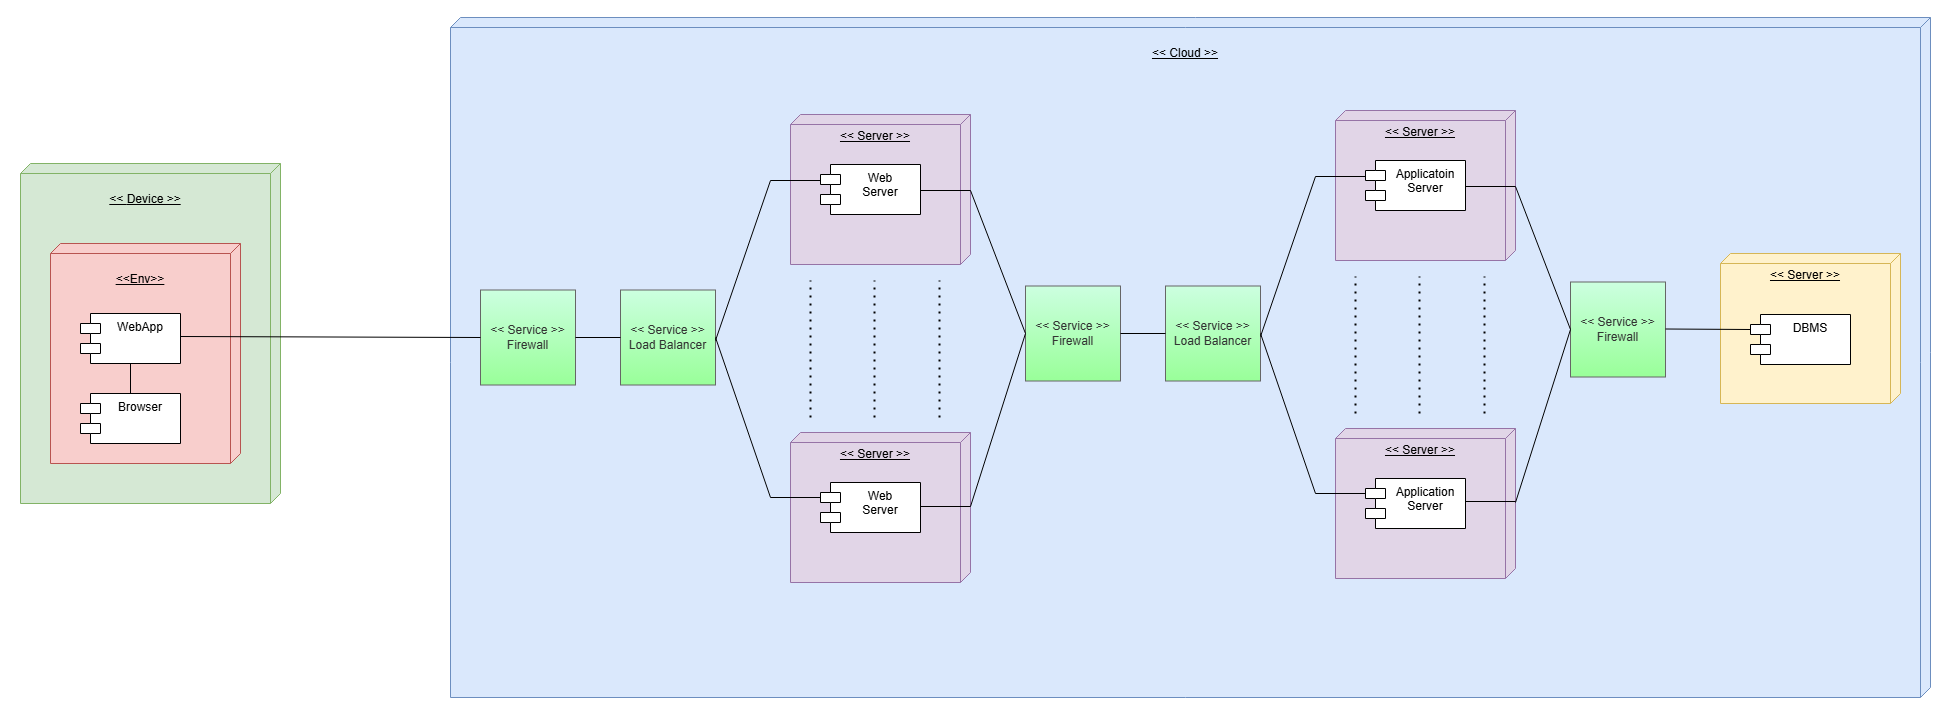
\includegraphics[scale = 0.33]{DD_figures/SingleDiagrams/DeploymentView.png}
    \caption{Component Diagram of the S\&C server subsystem}
    \centering
\end{figure}

\subsection{Runtime View}
This section contains the sequence diagrams of the most important operations of the
system. The diagrams include the components that we have already described in the
previous section and the external ones that are involved in the operations.

Moreover, the authentication mechanism for each user at the beginning of each operation is not explicitly included. It's assumed that the authentication and authorization will be implemented using a token-based process. These tokens are sent to the users each time they log in. They must be included with each request that requires authentication or authorization.



\subsubsection*{Student Registers}
The diagram represented below shows the process of a Student creating an account to the S\&C website. First, the student compiles the sign-up form with all the requested information. After that, the form information is checked and if the parameter result is valid, it is stored in the DB and a new account is generated. From there, the University login service, related to the university that the Student inserted in the form, is shown. If the Student logs successfully in its university account the AuthenticationManager triggers the verification email through the EmailServiceProvider. 
\\Eventually, all the companies that advertise an internship that the system recognizes valid to recommend are notified of the new student subscription to the platform.
\begin{figure}[H]
\centering
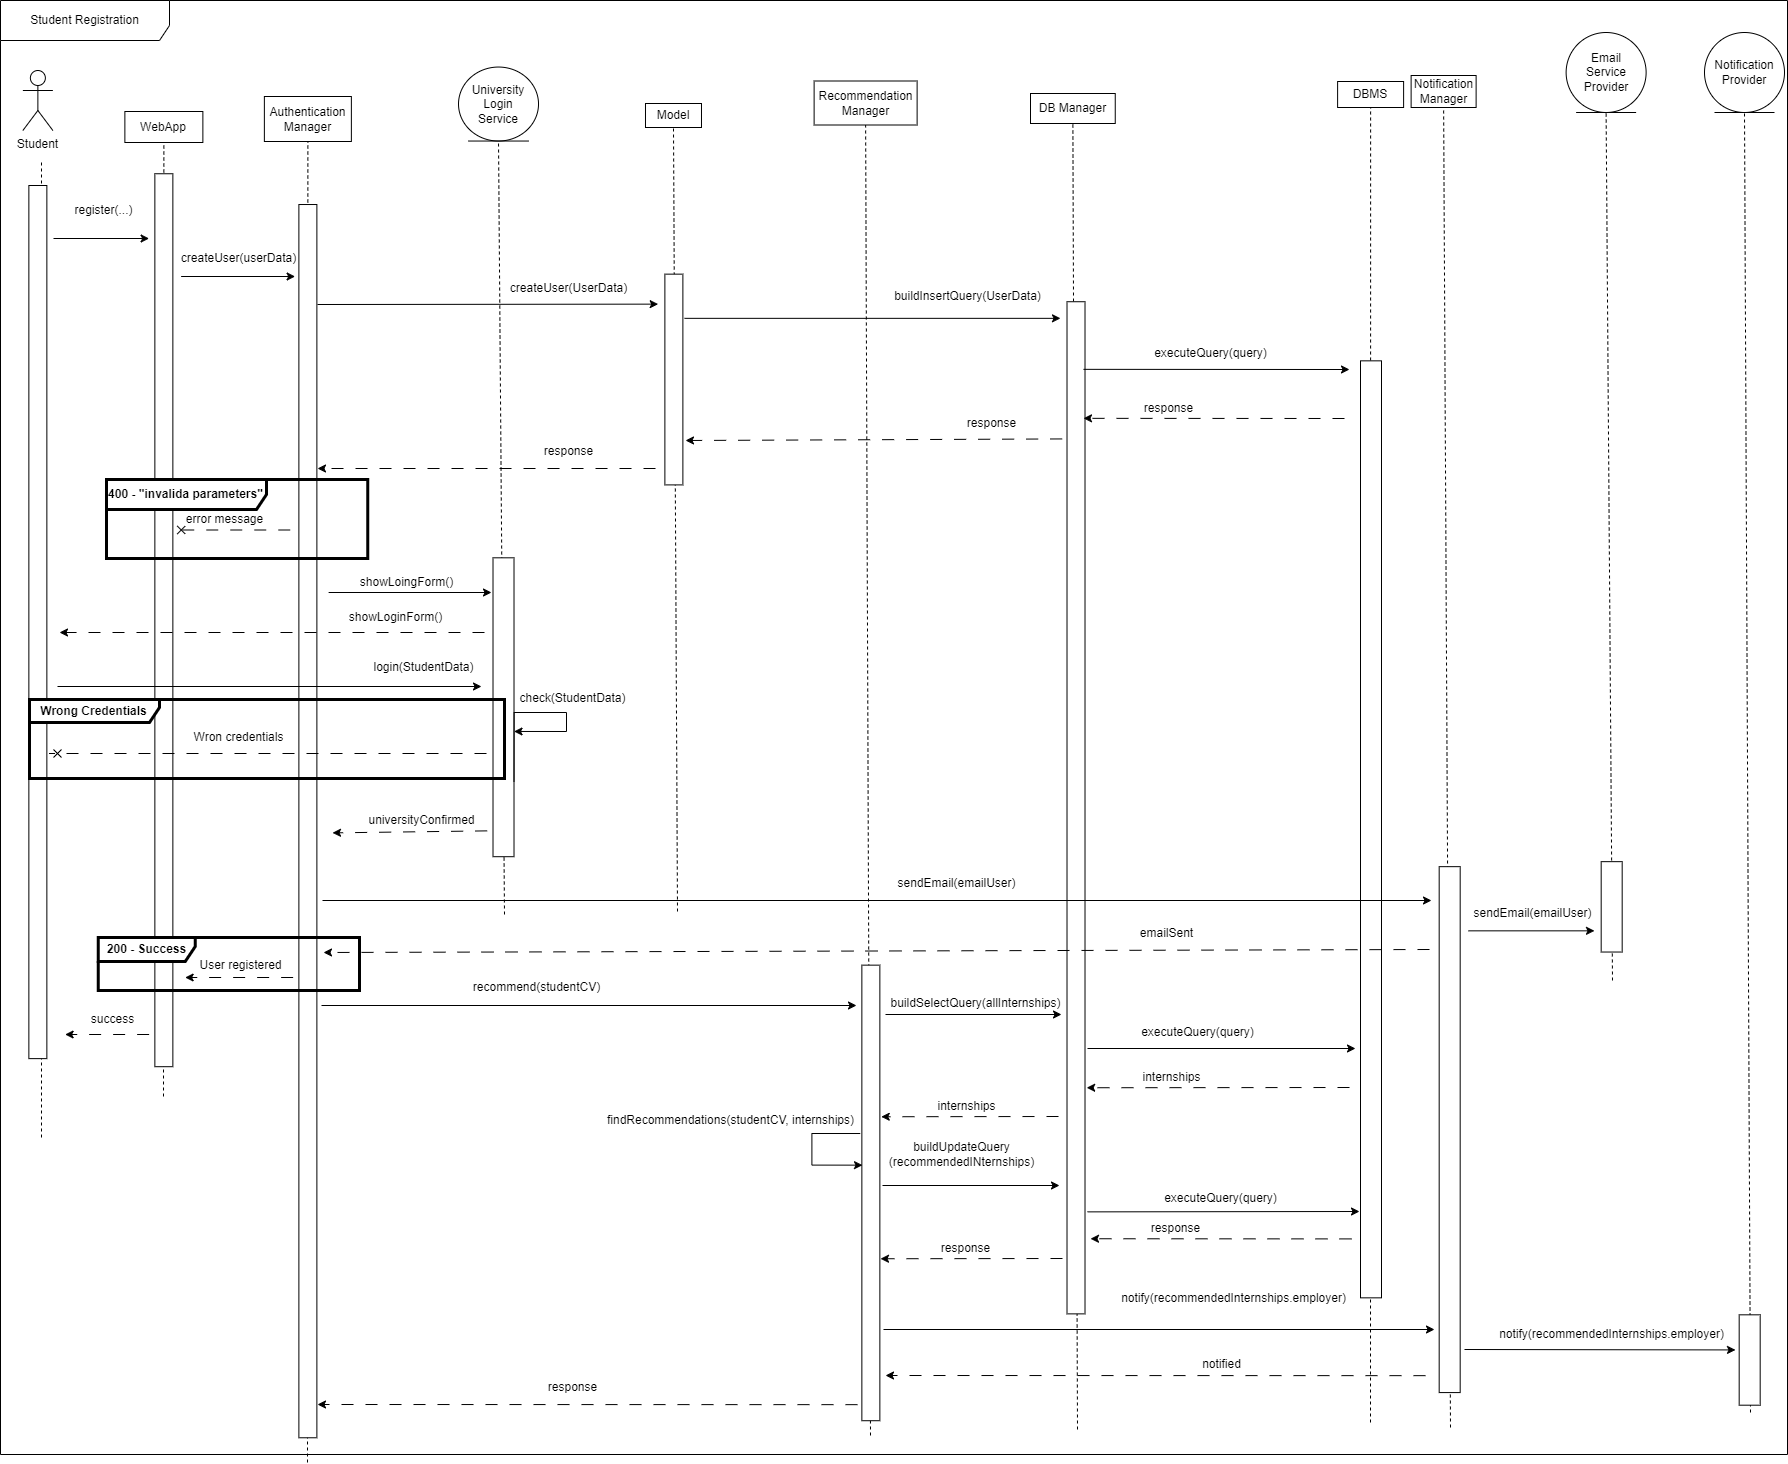
\includegraphics[scale = 0.28]{DD_figures/RuntimeView/StudentRegistrationRV.drawio.png}\\
\caption{Student Registers to S\&C}
\end{figure}

\newpage
\subsubsection*{Company Registers}
The diagram represented down below shows the process of a Company creating an account to the S\&C website. First, the Company compiles the sign up form with all the requested information, then, as the request is submitted through the proper API call, the AuthenticationManager component handles the request, and, if the parameters of the request were valid, the AuthenticationManager
triggers the verification email through the EmailServiceProvider.
\begin{figure}[H]
\centering
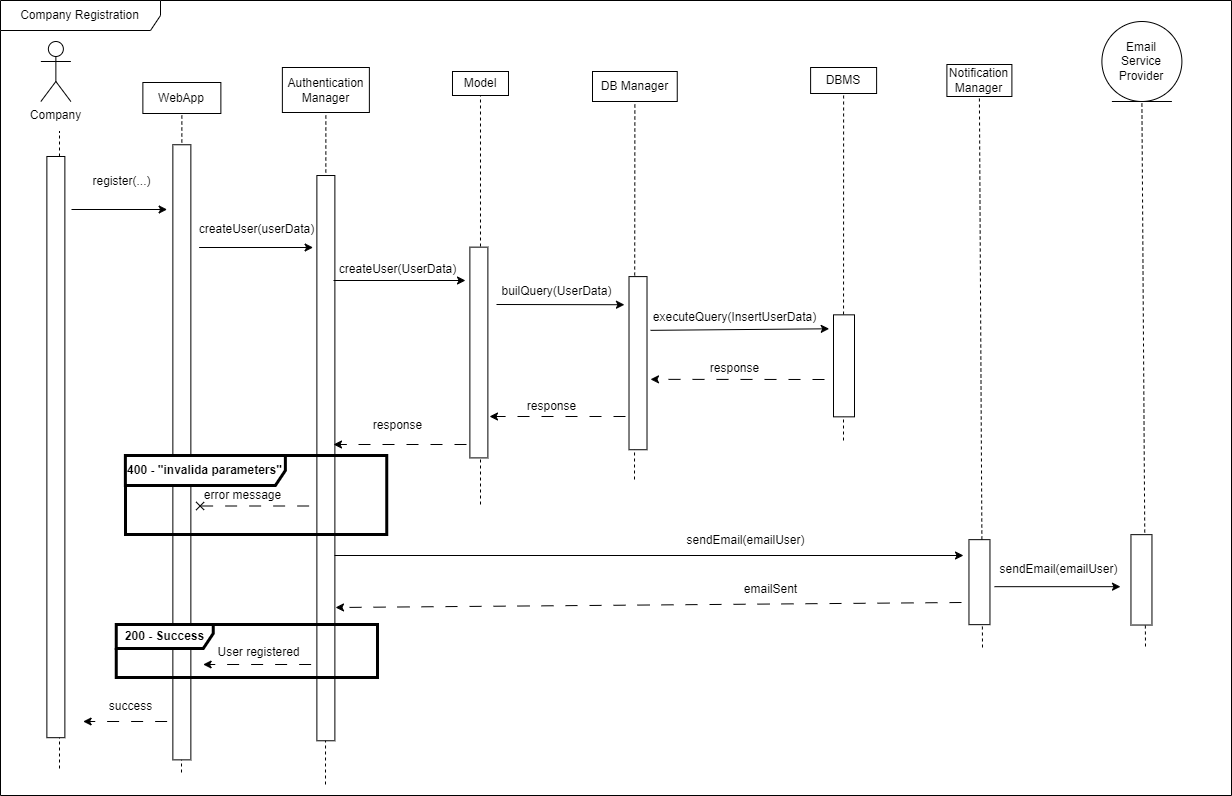
\includegraphics[scale = 0.35]{DD_figures/RuntimeView/CompanyRegistersRV.drawio.png}\\
\caption{Company Registers to S\&C}
\end{figure}

\newpage
\subsubsection*{University Registers}
The diagram represented down below shows the process of a University creating an account to the S\&C website. First, the University compiles the sign up form with all the requested information. From there, the University information is checked using the National Education Dictionary. If the information results correct, then the information is stored in the DB and a new University account is generated. At last, the AuthenticationManager
triggers the verification email through the EmailServiceProvider.
\begin{figure}[H]
\centering
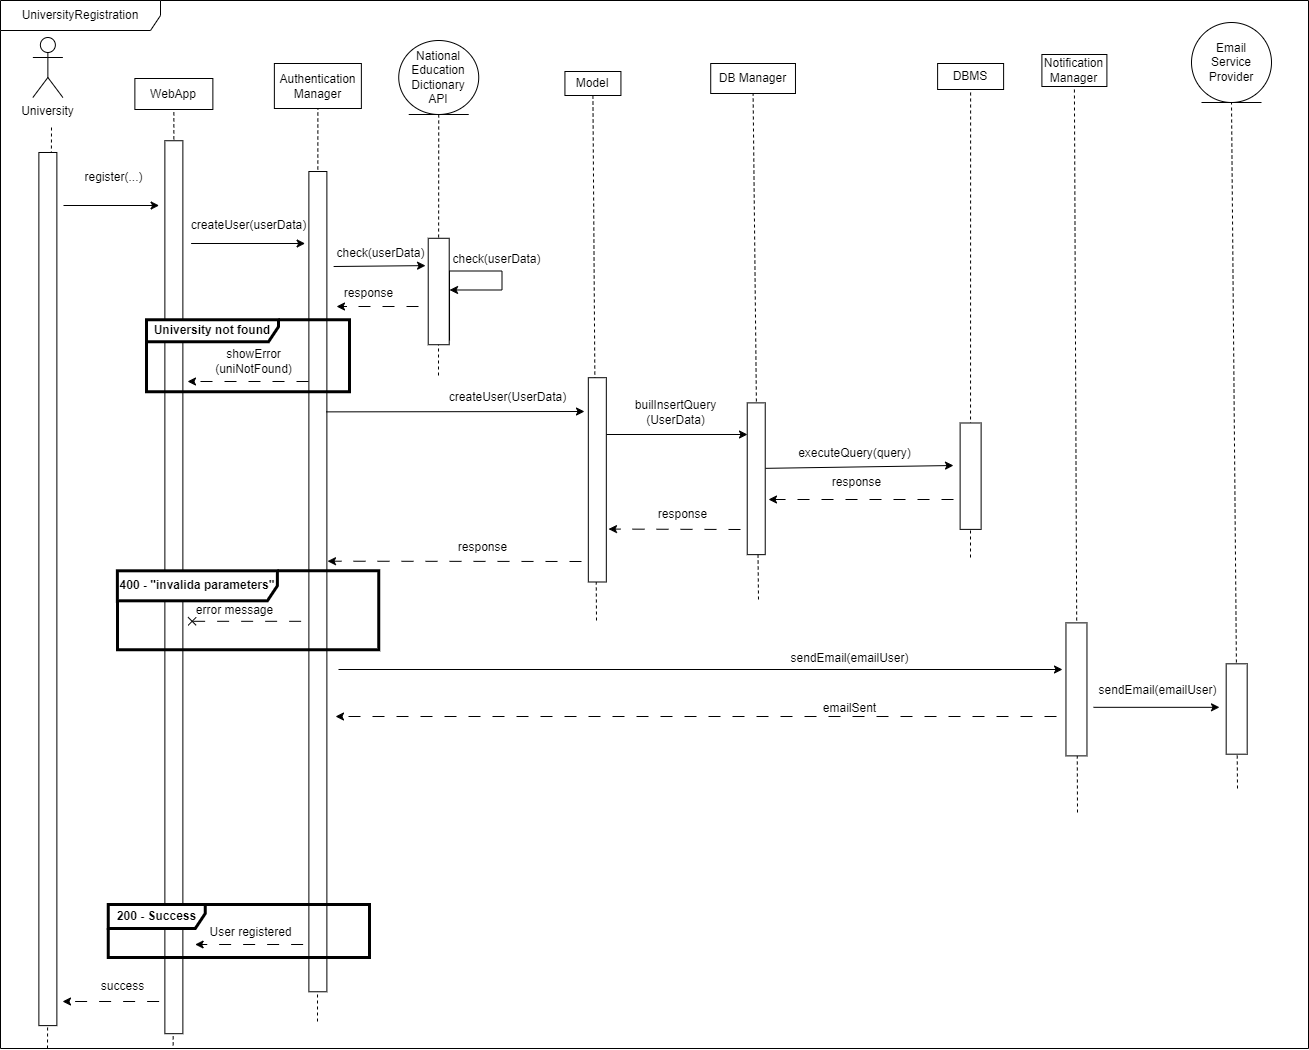
\includegraphics[scale = 0.30]{DD_figures/RuntimeView/UniversityRegistrationRV.drawio.png}\\
\caption{University Registers to S\&C}
\end{figure}
\newpage

\subsubsection*{User Views Template}
The diagram below shows the process of a User (either student or company) visualizing the suggested template by the platform.
\begin{figure}[H]
\centering
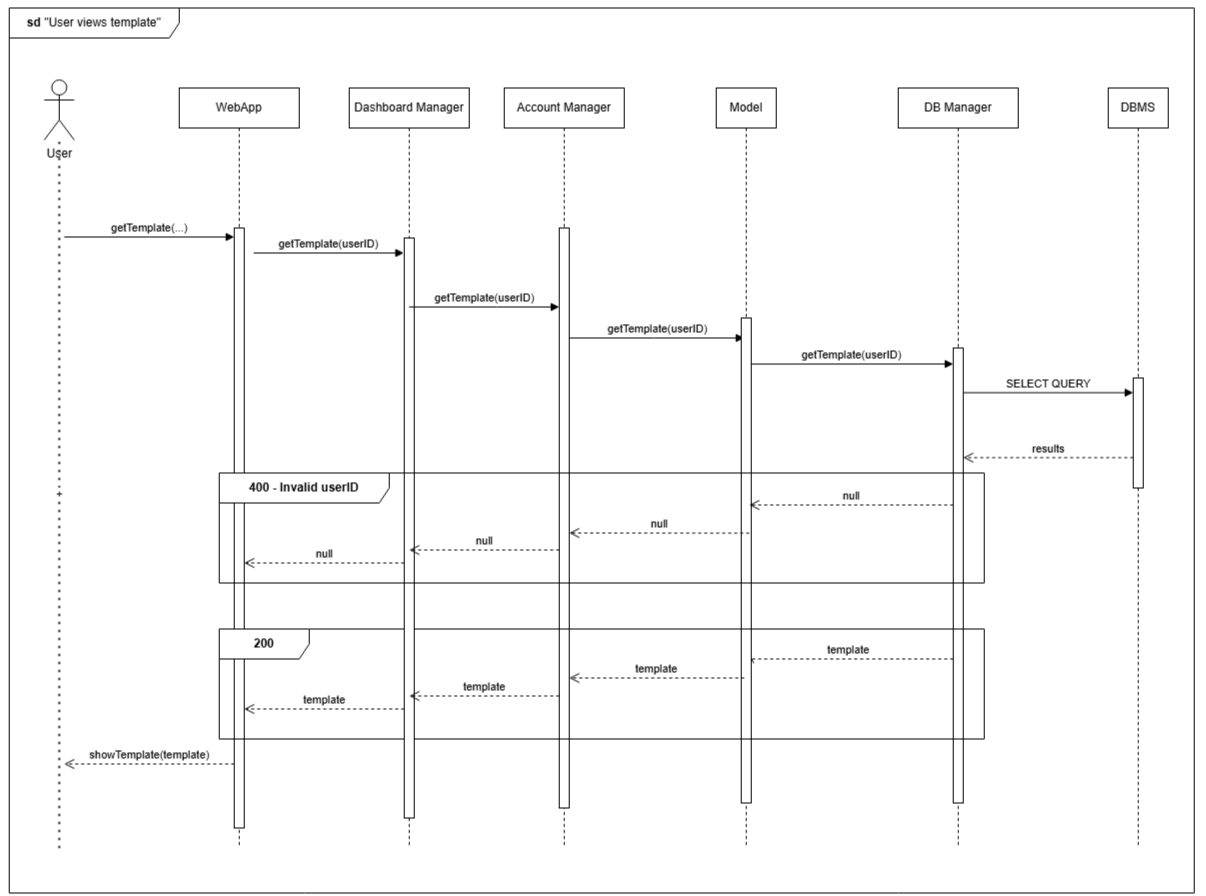
\includegraphics[scale = 0.5]{DD_figures/RuntimeView/UserViewsTemplateRV.png}\\
\caption{User Views Template}
\end{figure}
\newpage
\subsubsection*{ User Login}
    This diagram illustrates the login process within the system, regardless of the user type. We assumed that the user identifies their own type through interfaces and navigates the event flow using specific tabs and buttons to ultimately reach the login page. 
    
    The system verifies the user's credentials by querying with the database through the Authentication Manager. If the provided credentials (email and password) are incorrect, the user encounters an error message with error handling mechanisms  as shown in the diagram. However, if the credentials are valid, the authorized managers retrieve the user's Id from the database and redirect to the user's home page by using that.
    
    In addition, the diagram includes a loop representation to prevent that the potential database errors do not affect the system's overall functionality.
    \begin{figure}[H]
    \centering
    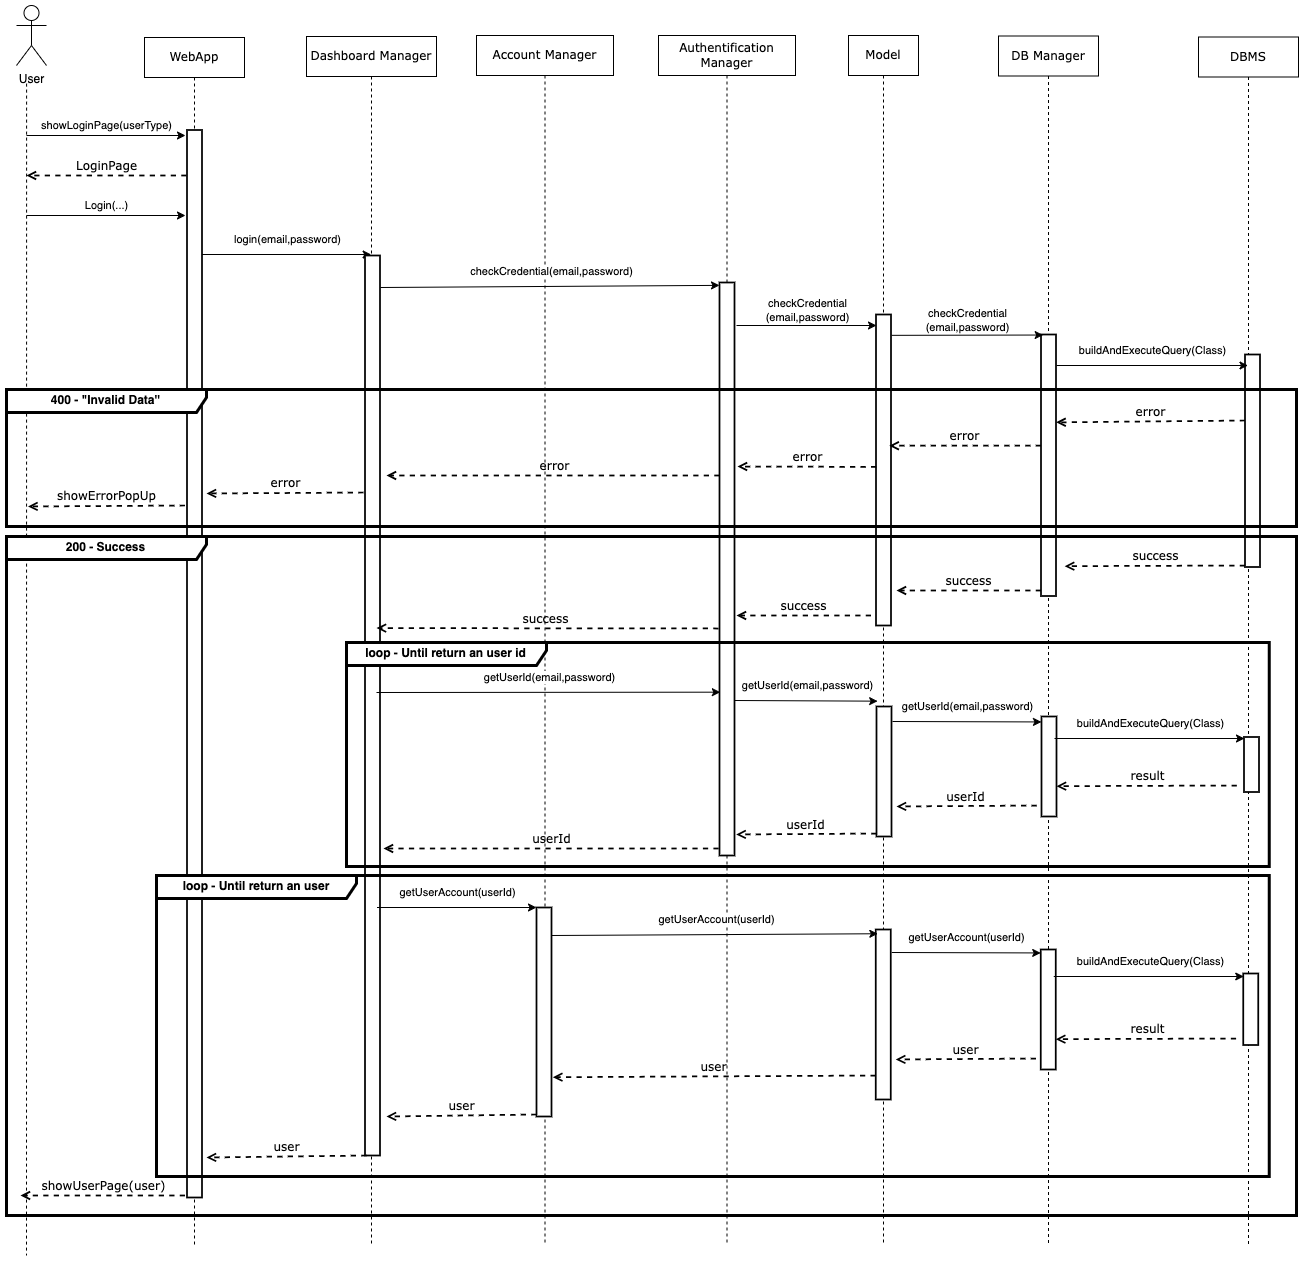
\includegraphics[scale = 0.30]{DD_figures/RuntimeView/UserLogin.drawio.png}
    \caption{User Login}
\end{figure}

\newpage

\subsubsection*{Student Updates CV}
The student initiates the process by uploading their CV, which is handled by the WebApp and subsequently passed to the Dashboard Manager, Account Manager, and Model components for validation and processing. If the data are valid, the CV is updated in the database using a query managed by the DB Manager and the DBMS. Upon successful update, the Recommendation Manager generates internship recommendations based on the updated CV, retrieving relevant internships and notifying associated employers. In case of an error (e.g., incorrect data), the system responds with an appropriate error message. Notifications are sent to employers through the Notification Provider, ensuring the flow of updates and recommendations.
\begin{figure}[H]
\centering
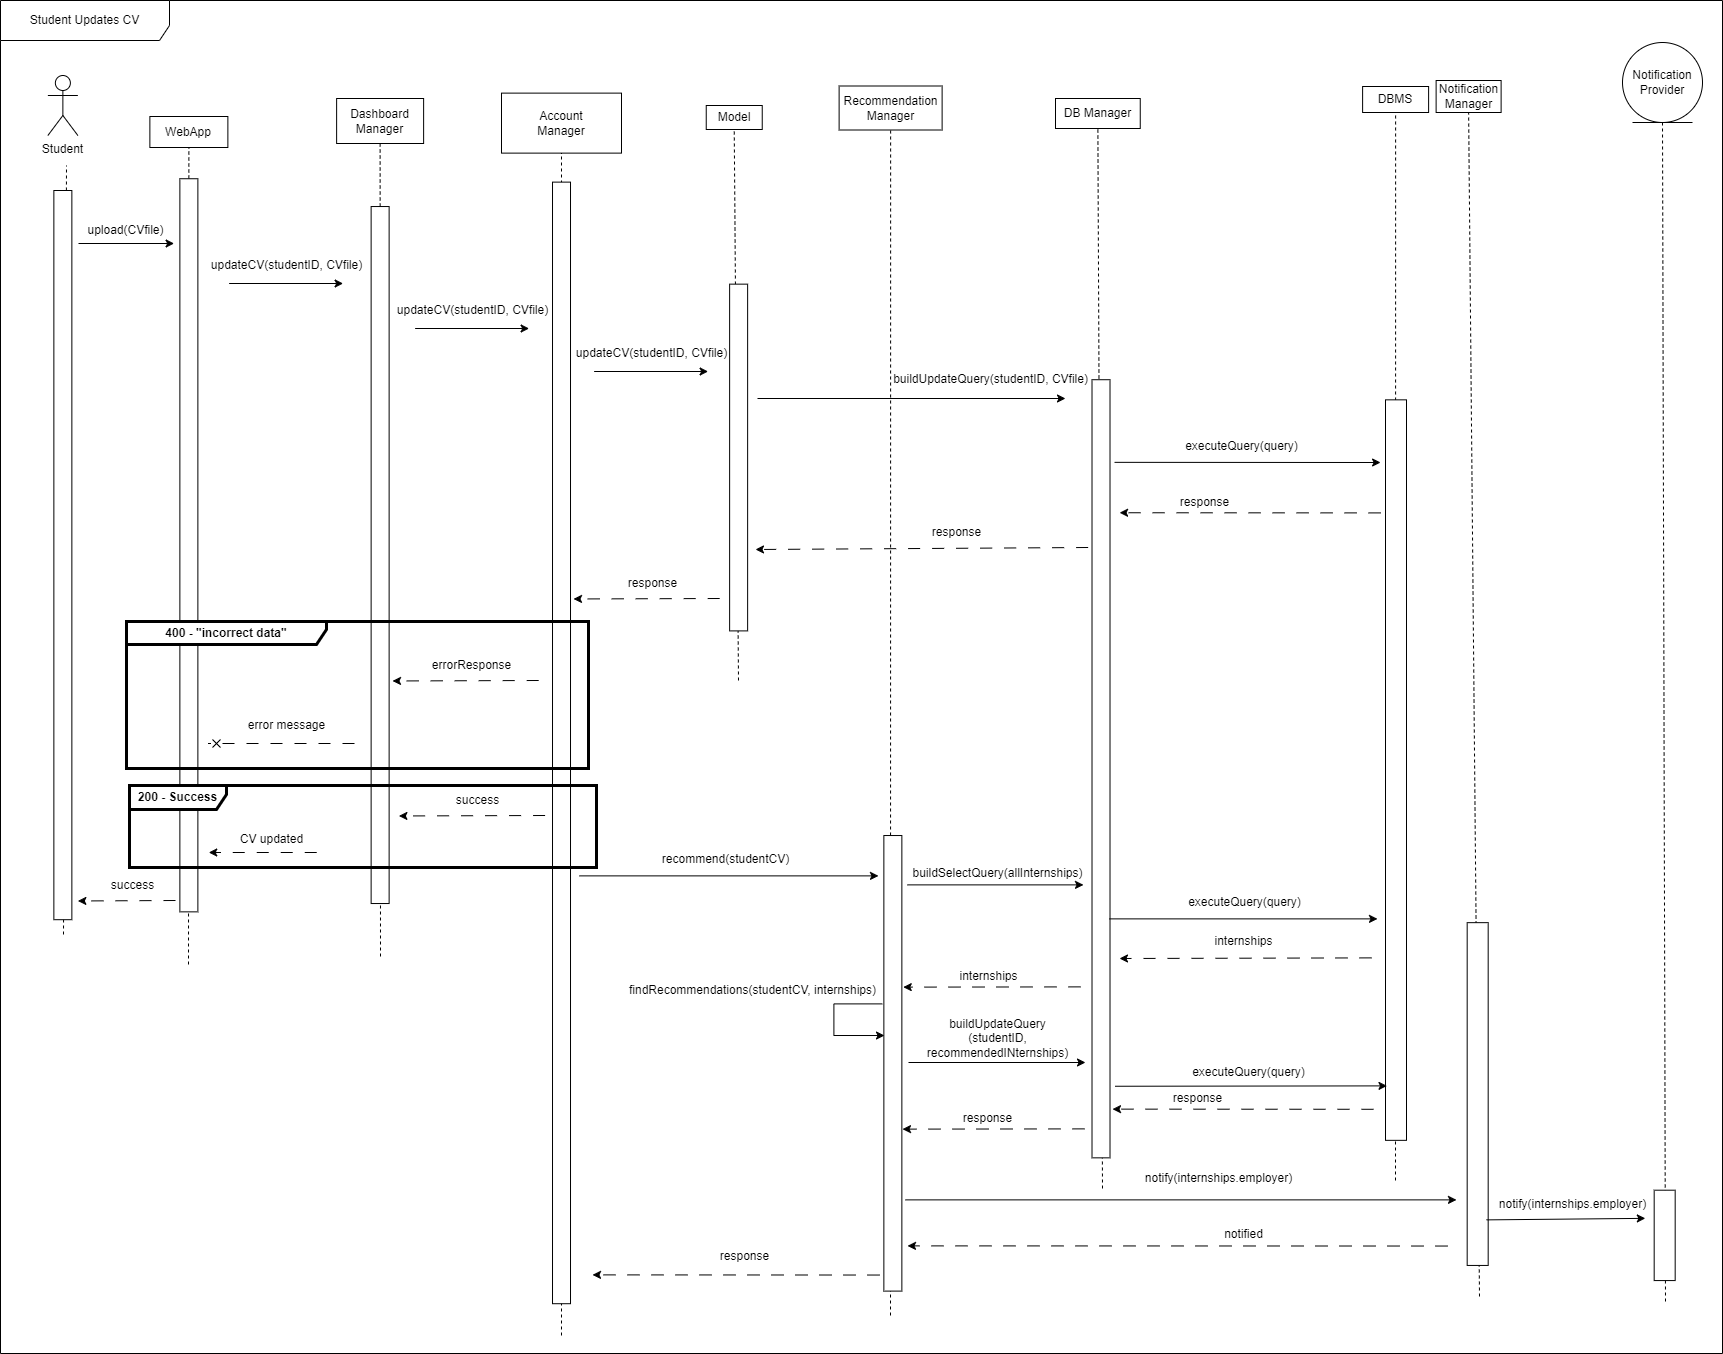
\includegraphics[scale = 0.28]{DD_figures/RuntimeView/StudentUpdatesCV_RV.drawio.png}\\
\caption{Student Updates CV}
\end{figure}

\newpage

\subsubsection*{Student Changes University}
The student begins the process by submitting a form with their new email associated to their new university to the WebApp. The form data are forwarded to the Dashboard Manager and Account Manager for validation and processing. If the parameters are valid, the system interacts with the University Login Service to verify the student's credentials and confirm the university enrollment. Once confirmed, the Account Manager updates the student's university information in the database by sending a query to the DB Manager, which is executed by the DBMS. Upon successful update, the system sends a success response to the student.
In case of errors, such as invalid parameters or incorrect credentials, the system returns an appropriate error message through the WebApp. This ensures clear communication with the student at every stage of the process.
\begin{figure}[H]
\centering
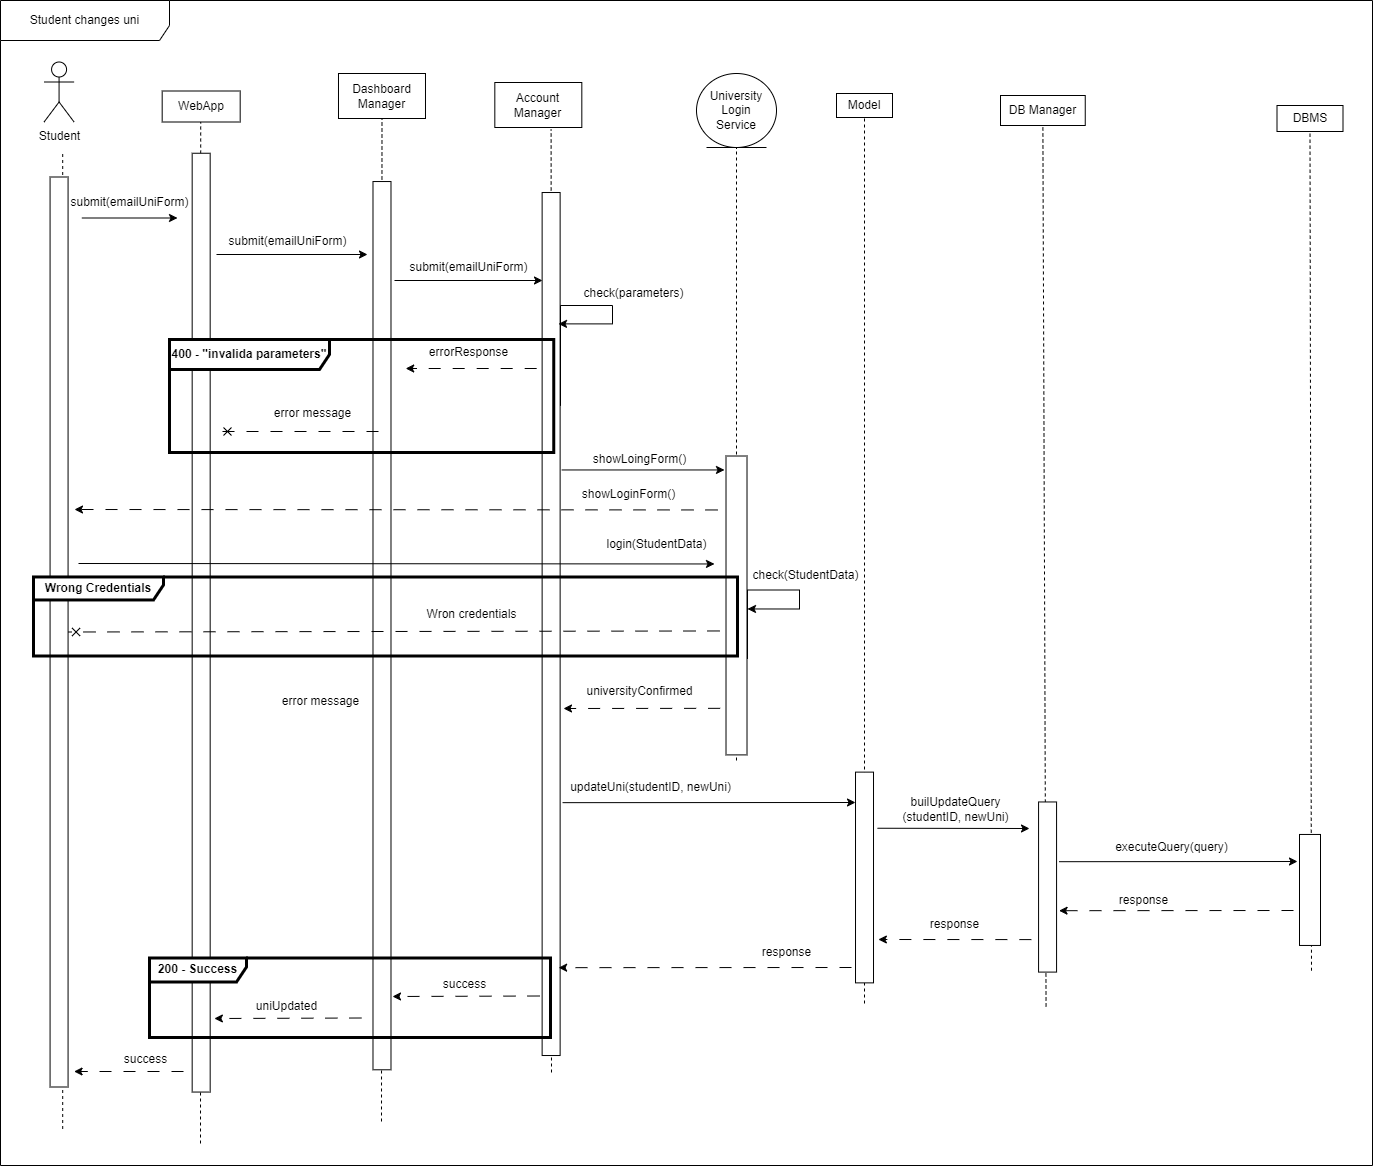
\includegraphics[scale = 0.35]{DD_figures/RuntimeView/StudentChangesUniversityRV.drawio.png}\\
\caption{Student Changes University}
\end{figure}
\newpage

\subsubsection*{ Company Posts An Internship Advertisement}  
This diagram illustrates the scenario of posting an internship advertisement through the system according to the company's needs. The process begins with the company navigating to the appropriate page via the system interfaces to initiate advertisement creation. We assumed that all required fields within the interface are completed. The system first receives the information and advertisement details filled out by the company user and save them into the DBMS through the relevant managers using the parameters adInfo(advertisementInfo) and companyId. Upon successful creation of the advertisement within the system, relevant student profiles are identified and recommended through the recommendation manager for the advertisement, and these suggested students are saved to the database. Furthermore, the system notifies the identified students of the newly created advertisement, which might align with their interests, through the notification manager and provider. The diagram also incorporates error-handling mechanisms to improve system security and efficiency.

\begin{figure}[H]
    \centering
    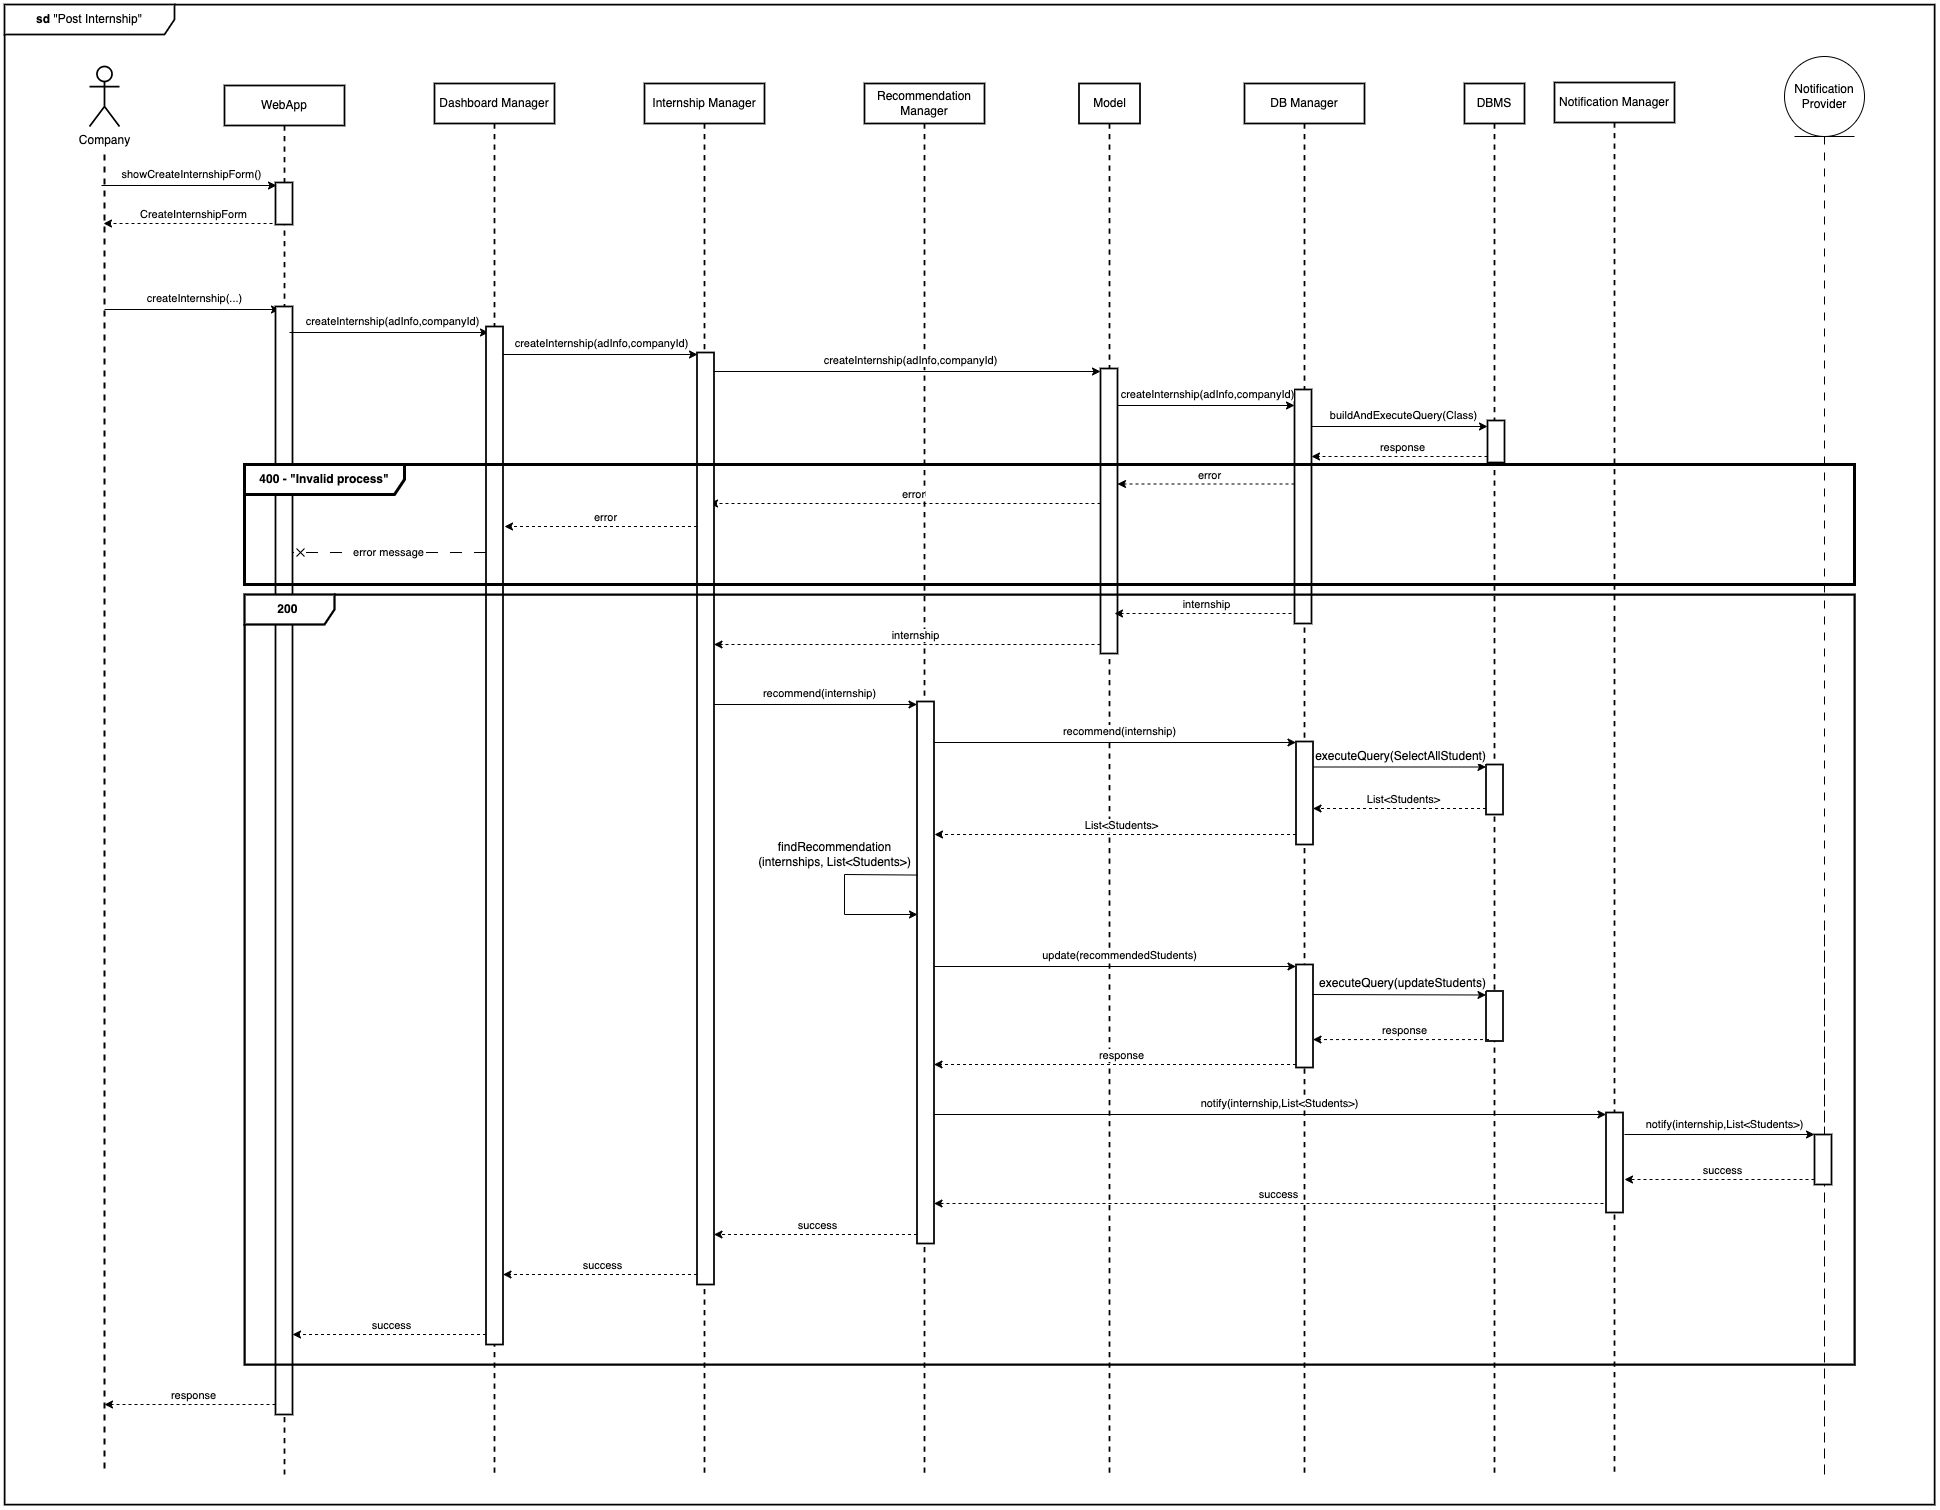
\includegraphics[scale = 0.25]{DD_figures/SingleDiagrams/postInternship.drawio.png}
    \caption{Company Create Internship}
    \centering
\end{figure}
\newpage

\subsubsection*{User Views Relevant Internships}
The diagram below shows the process of a user visualizing the list of internships he's interested in. \\
In the case of a University, it retrieves all the internships the students from that university were selected for
\begin{figure}[H]
\centering
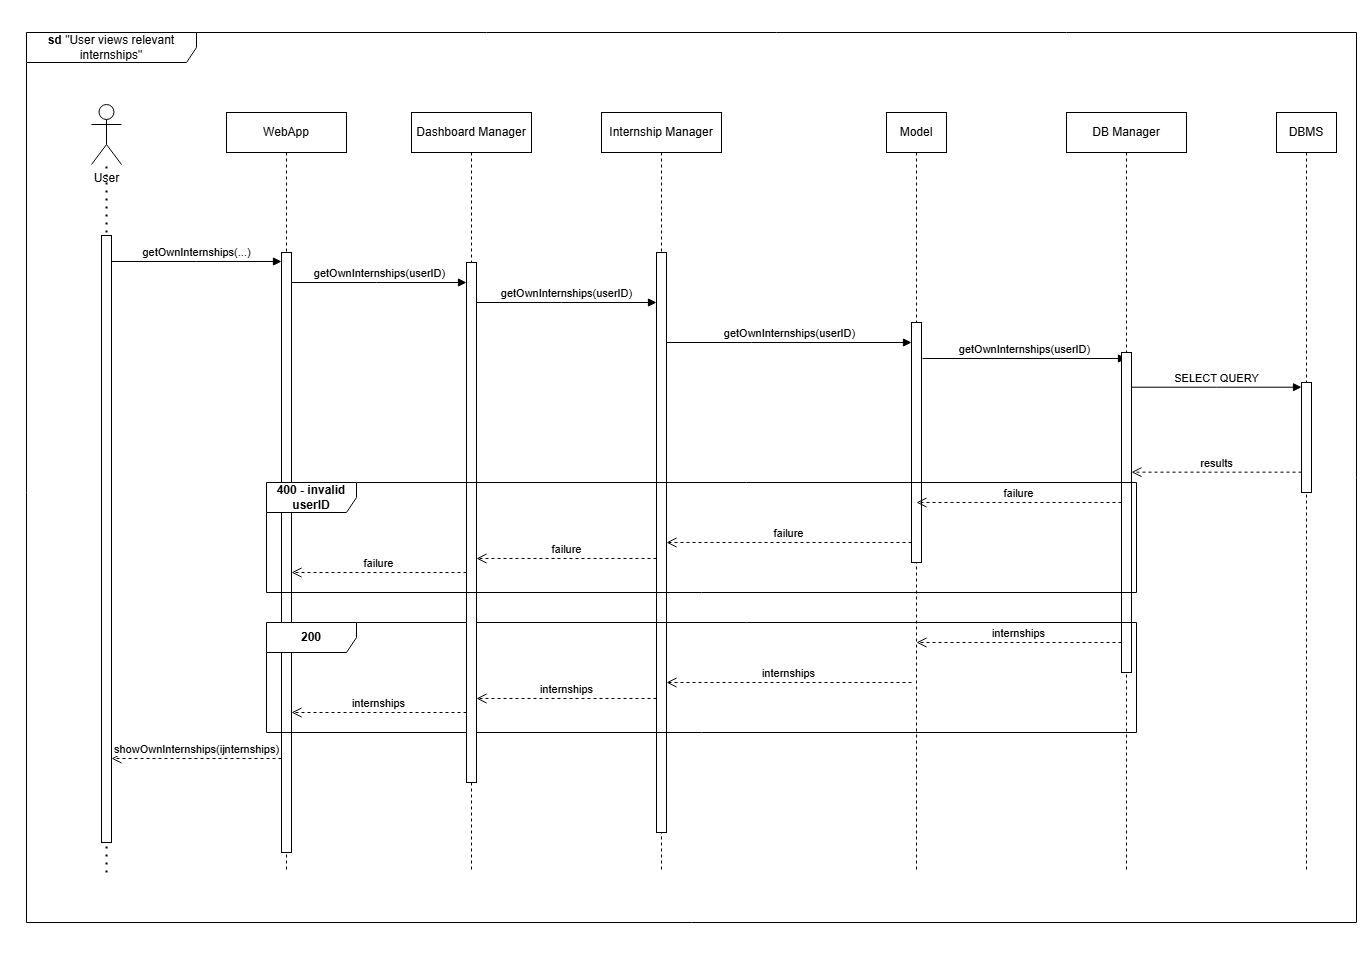
\includegraphics[scale = 0.4]{DD_figures/RuntimeView/UserViewsRelevantInternshipsRV.png}\\
\caption{User Views Relevant Internships}
\end{figure}

\newpage

\subsubsection*{ Student Views and Apply For The Advertisement} 
This diagram illustrates the scenario in which students utilize the system’s homepage interface to list general internship advertisements and view their details. The process begins with the student accessing the system’s homepage, where the system retrieves a list of previously shared advertisements from the Database Management System (DBMS) and presents it to the user. If the list contains advertisements, we assumed that the student will proceed to view the details of a selected advertisement as part of the scenario. 
\begin{figure}[H]
    \centering
    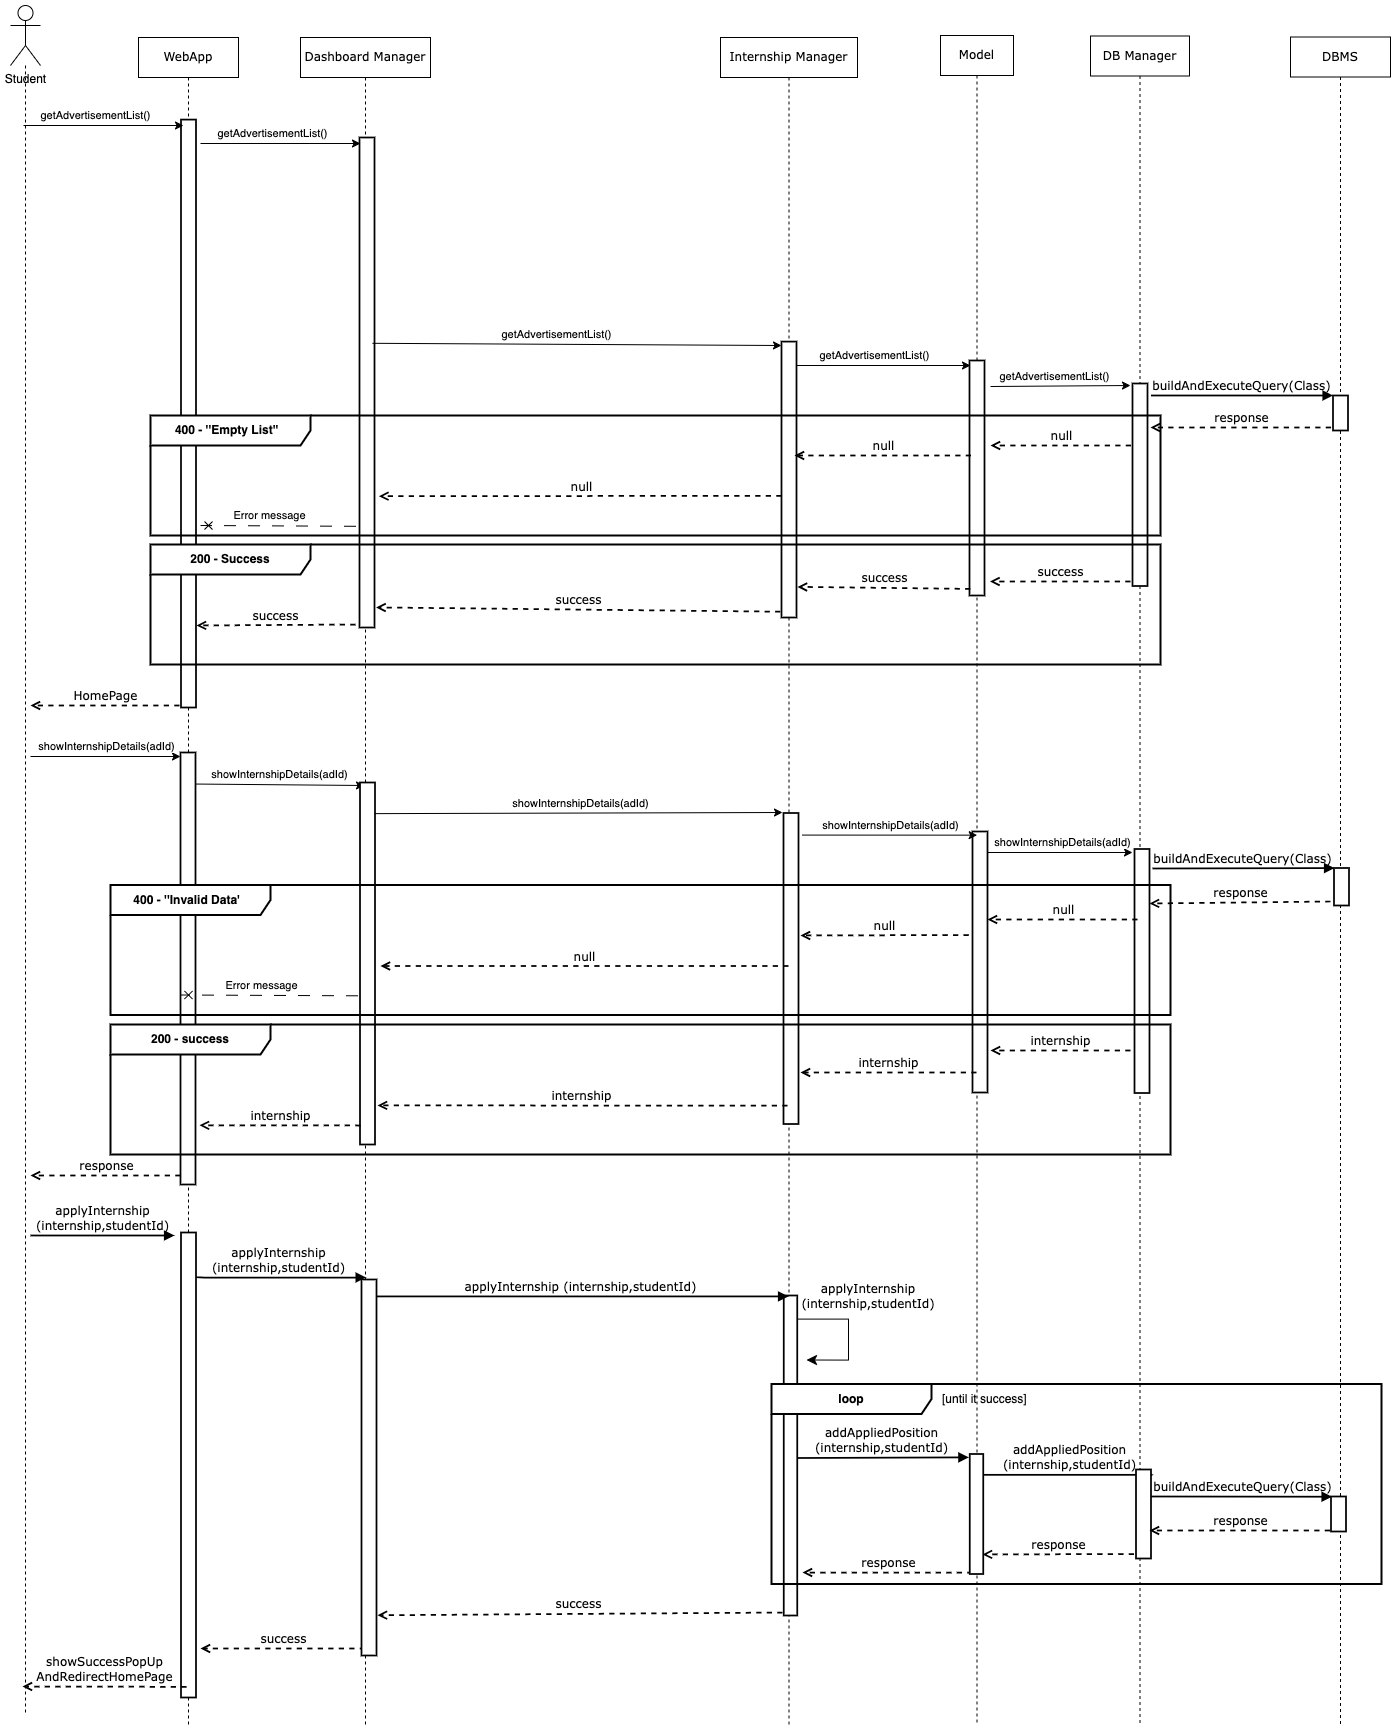
\includegraphics[scale = 0.25]{DD_figures/RuntimeView/studentViewInternship.drawio.png}
    \caption{Student Views Advertisements}
    \centering
\end{figure}
\newpage

\subsubsection*{Company Views Recommended and Applying Students} 
This diagram represents the scenario in which companies view a list of advertisements previously shared through their own profiles. The company navigates to the "Manage Internship" page, and the system sends a request to the DBMS through the relevant managers using the companyId parameter. The system retrieves the list of advertisements and displays it on the interface. The diagram also incorporates a condition to check whether any advertisements exist. If the list is available, the scenario proceeds with the company selecting one of the advertisements.
\begin{figure}[H]
    \centering
    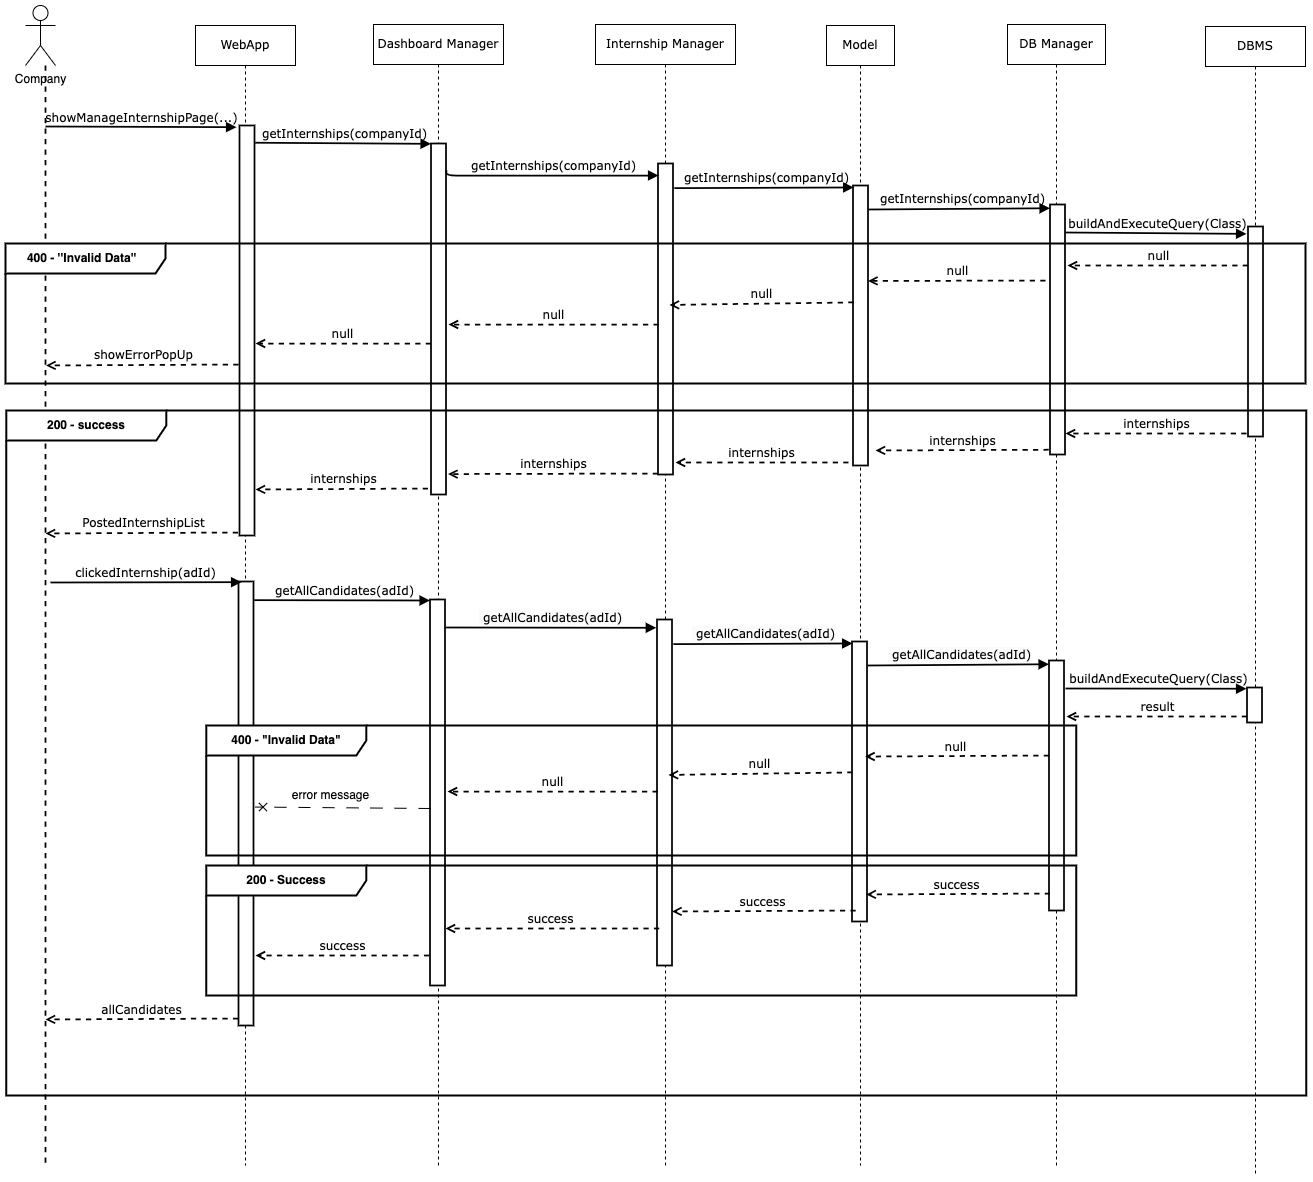
\includegraphics[scale = 0.25]{DD_figures/RuntimeView/companyViewStudent.drawio.png}
    \caption{Company Views Recommended and Applying Students}
    \centering
\end{figure}

\newpage

\subsubsection*{ Company Views The Student Details and Accepts} 
This diagram is presented as a continuation of the scenario shown in Figure 19. In summary, the company has accessed the advertisements they previously shared and navigated to the desired advertisement cell. In this scenario, we assumed that the company selects a student's profile from the "All Candidates" list via the interface. 
\begin{figure}[H]
    \centering
    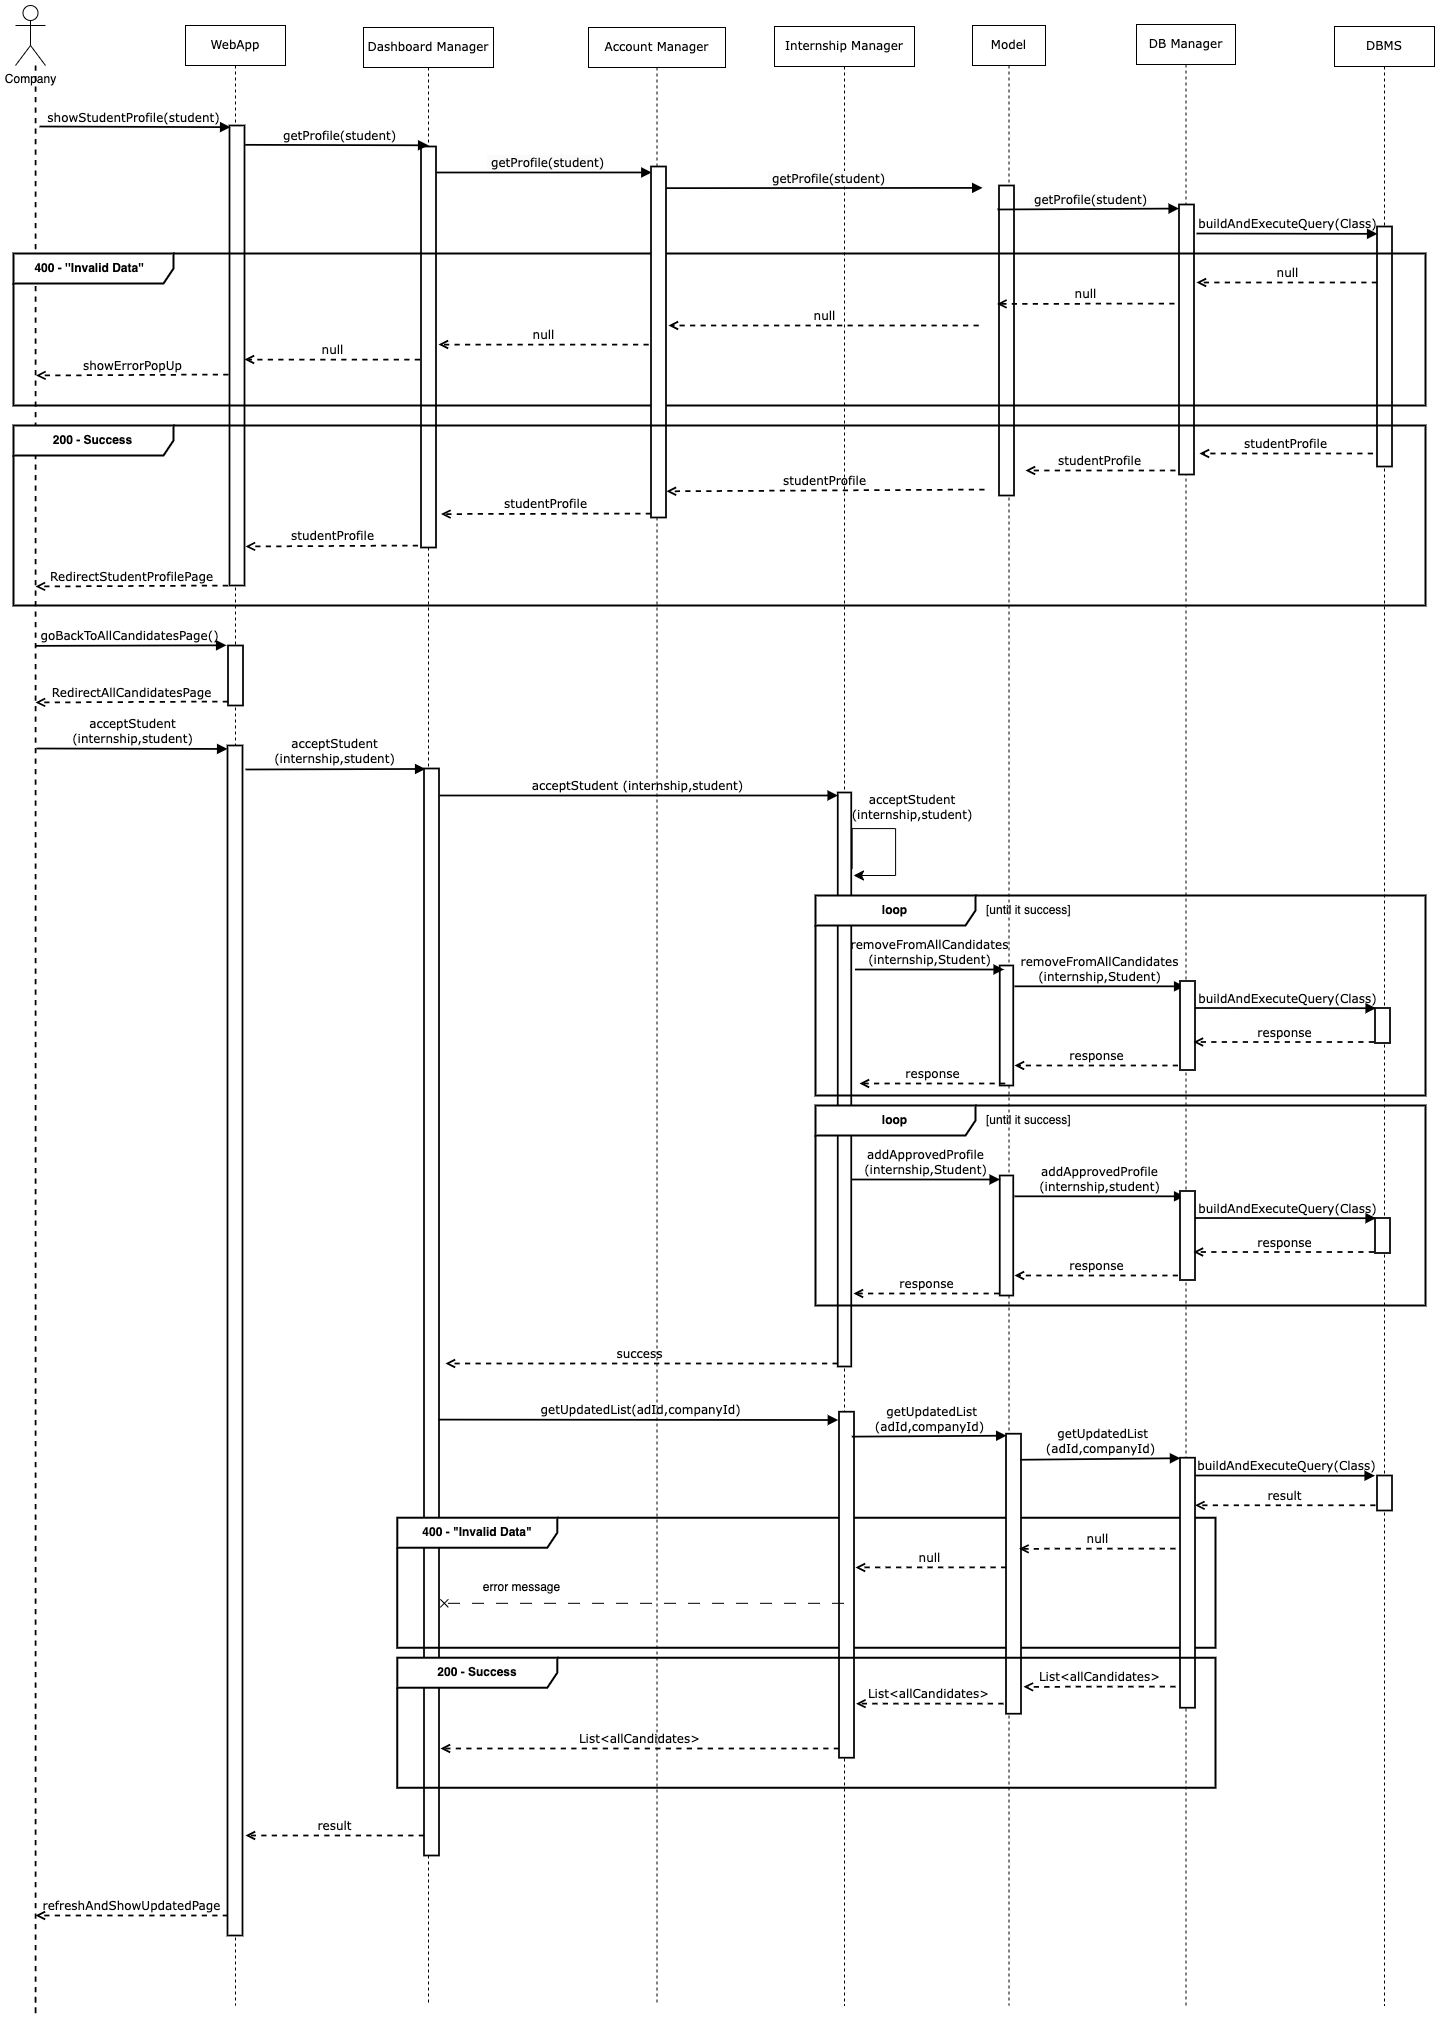
\includegraphics[scale = 0.7]{DD_figures/RuntimeView/companyViewStudentDetails.drawio.png}
    \caption{Company Views The List of Student}
    \centering
\end{figure}

\newpage

\subsubsection*{User Accepts}
The diagram below shows the process of a User (either student or company) accepting the other. Both studentID and internshipID are needed for the operation.
\begin{figure}[H]
\centering
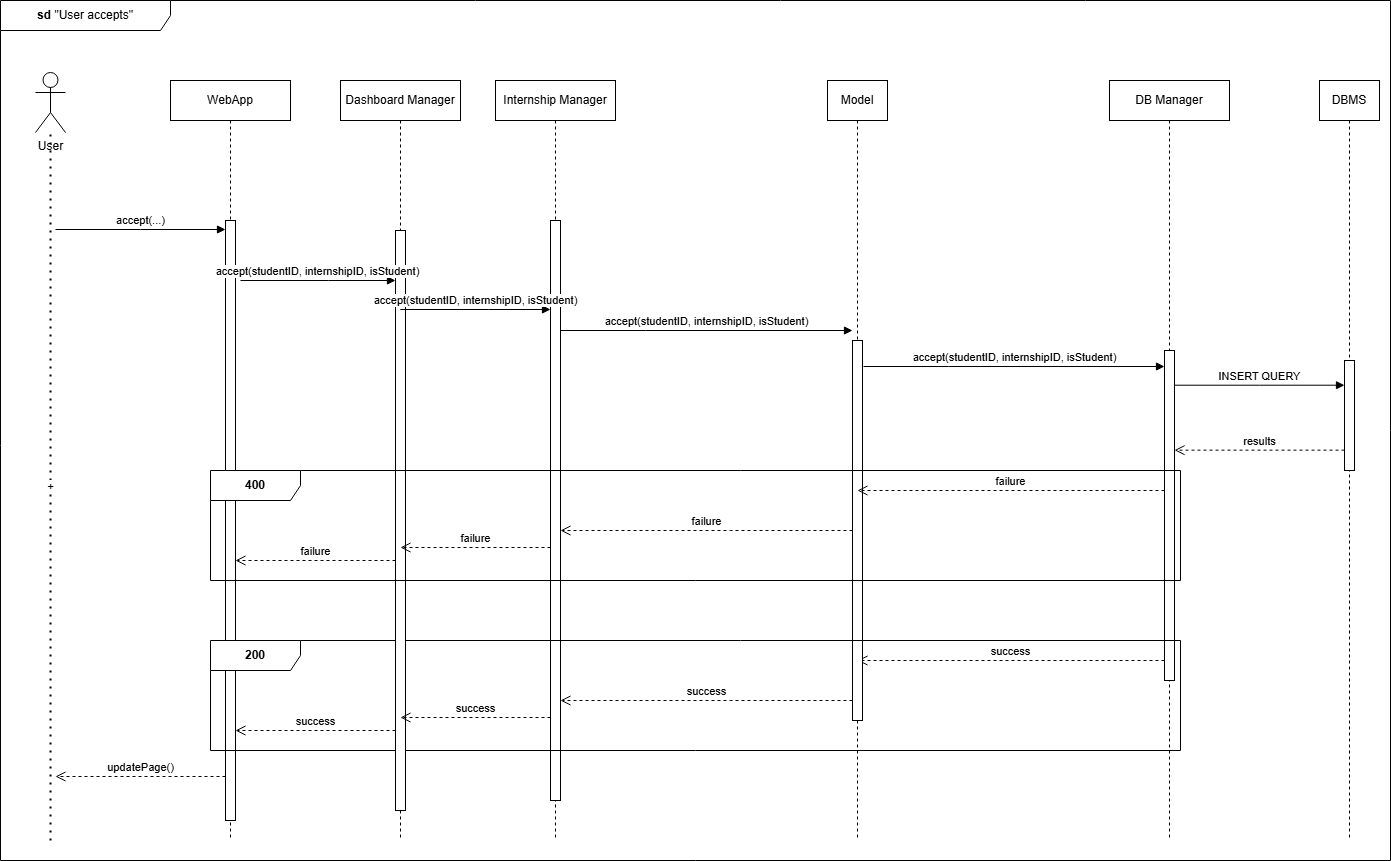
\includegraphics[scale = 0.4]{DD_figures/RuntimeView/UserAcceptsRV.png}\\
\caption{User Accepts}
\end{figure}
\newpage

\subsubsection*{ User Gives Feedback About Recommendations}  

The diagram demonstrates the process of feedback on recommendations, regardless of their user type. This attribute can be use onyly for student and company user types, so the diagram shows some conditions to handle error for unauthorized user types.

The process begins with functions including the internship class (containing attributes such as companyId, advertisementId, or studentId) , userId and a boolean response data type. The updateRecommendationStatus function allows each user to provide feedback only once, and it records that in the database. In addition, the system analyzes the feedback collected to optimize the recommendation mechanism, allowing the system to offer more accurate and personalized suggestions over time.
    \begin{figure}[H]
    \centering
    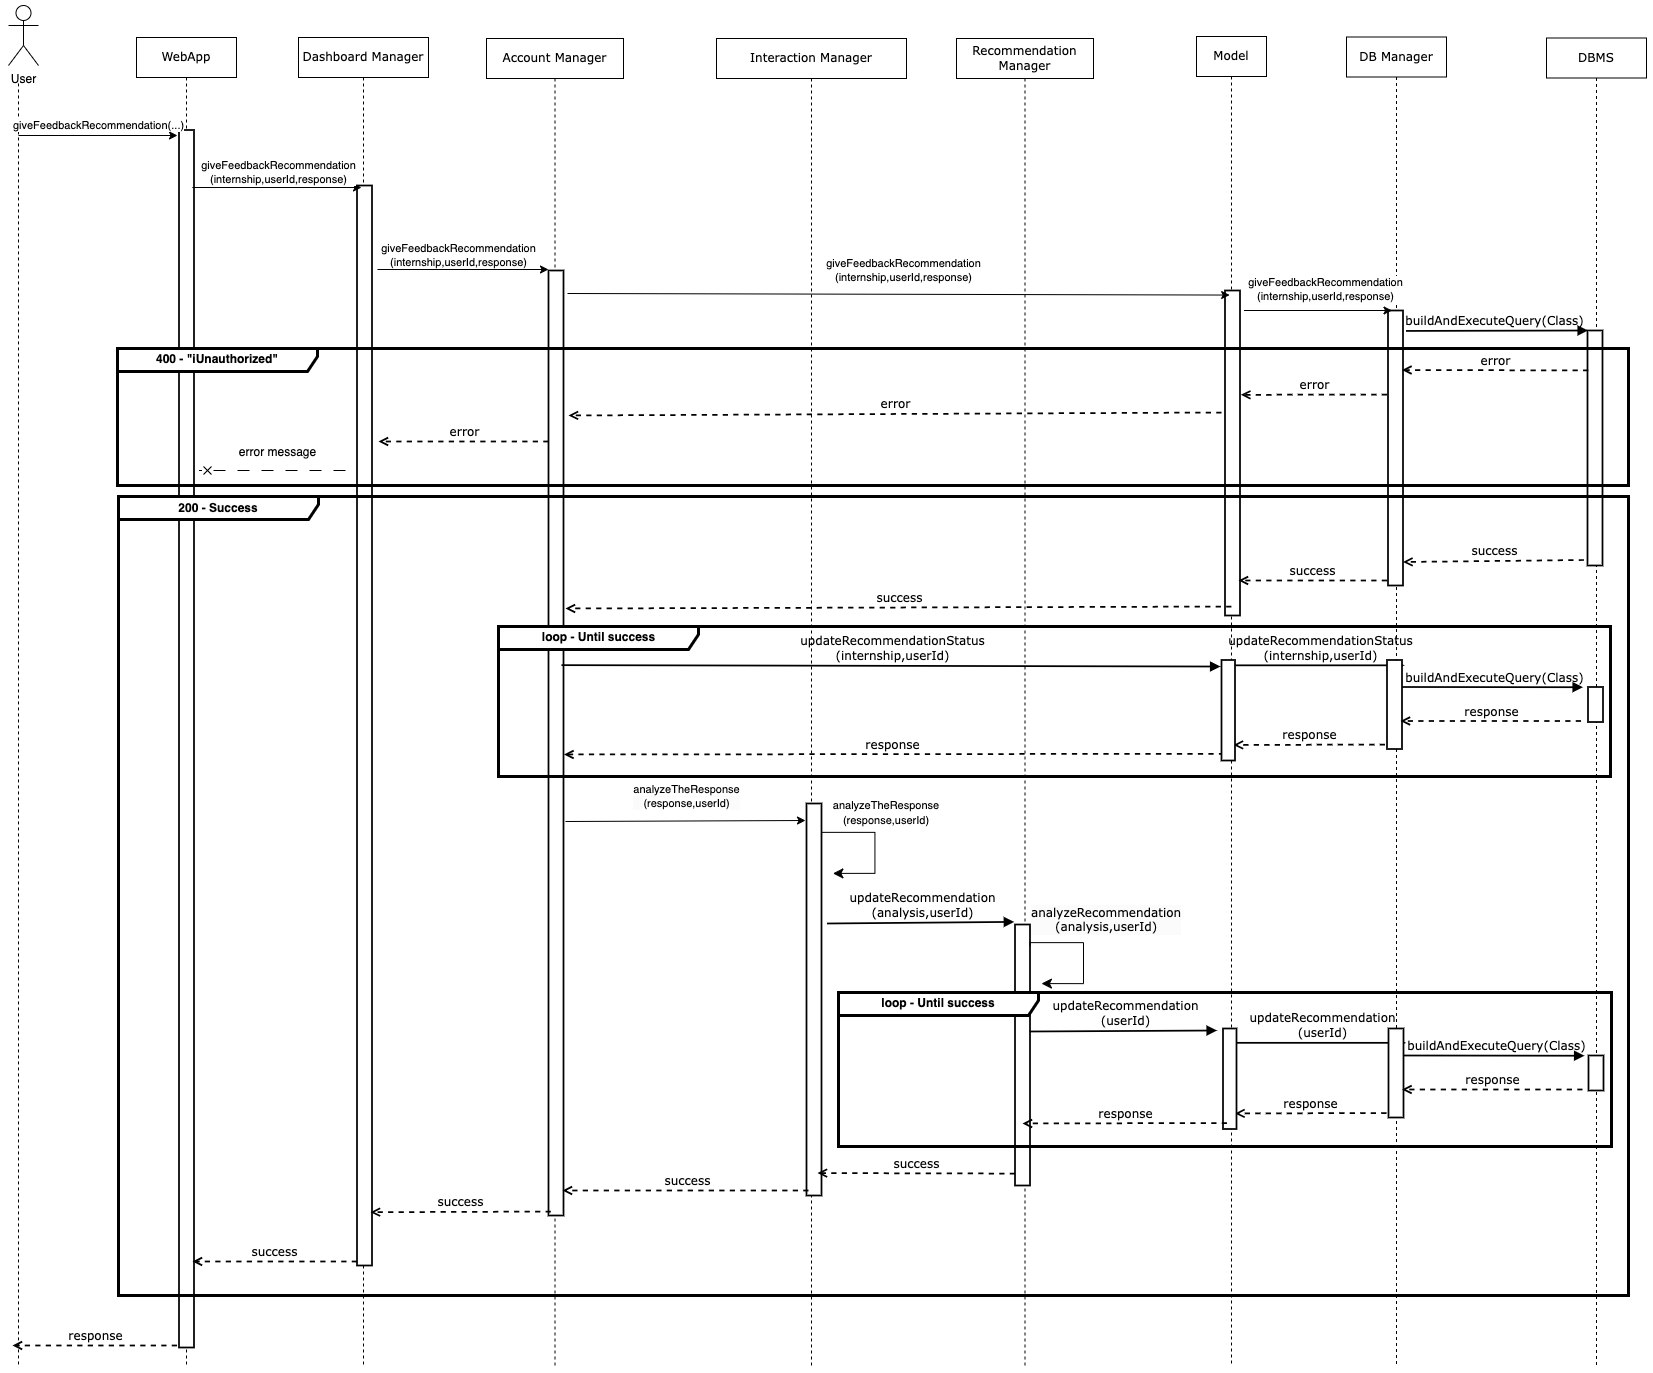
\includegraphics[scale = 0.25]{DD_figures/RuntimeView/userGiveFeedbackRecomm.drawio.png}
    \caption{User Recommendation Feedback}
\end{figure}

\newpage
\subsubsection*{Company Sends Interview Form}
The company initiates the process by submitting an interview form to the WebApp. The form data is forwarded to the Dashboard Manager, Internship Manager, and Model components for validation and processing. If the parameters are valid, the system builds an insert query and sends it to the DB Manager, which is then executed by the DBMS to save the interview time slots. Upon successful saving, the system retrieves the list of candidates for the interview from the database and sends them notifications about the available time slots. In case of errors, such as invalid parameters, the system returns an appropriate error message through the WebApp. This ensures clear communication and efficient execution of the interview scheduling process.
\begin{figure}[H]
\centering
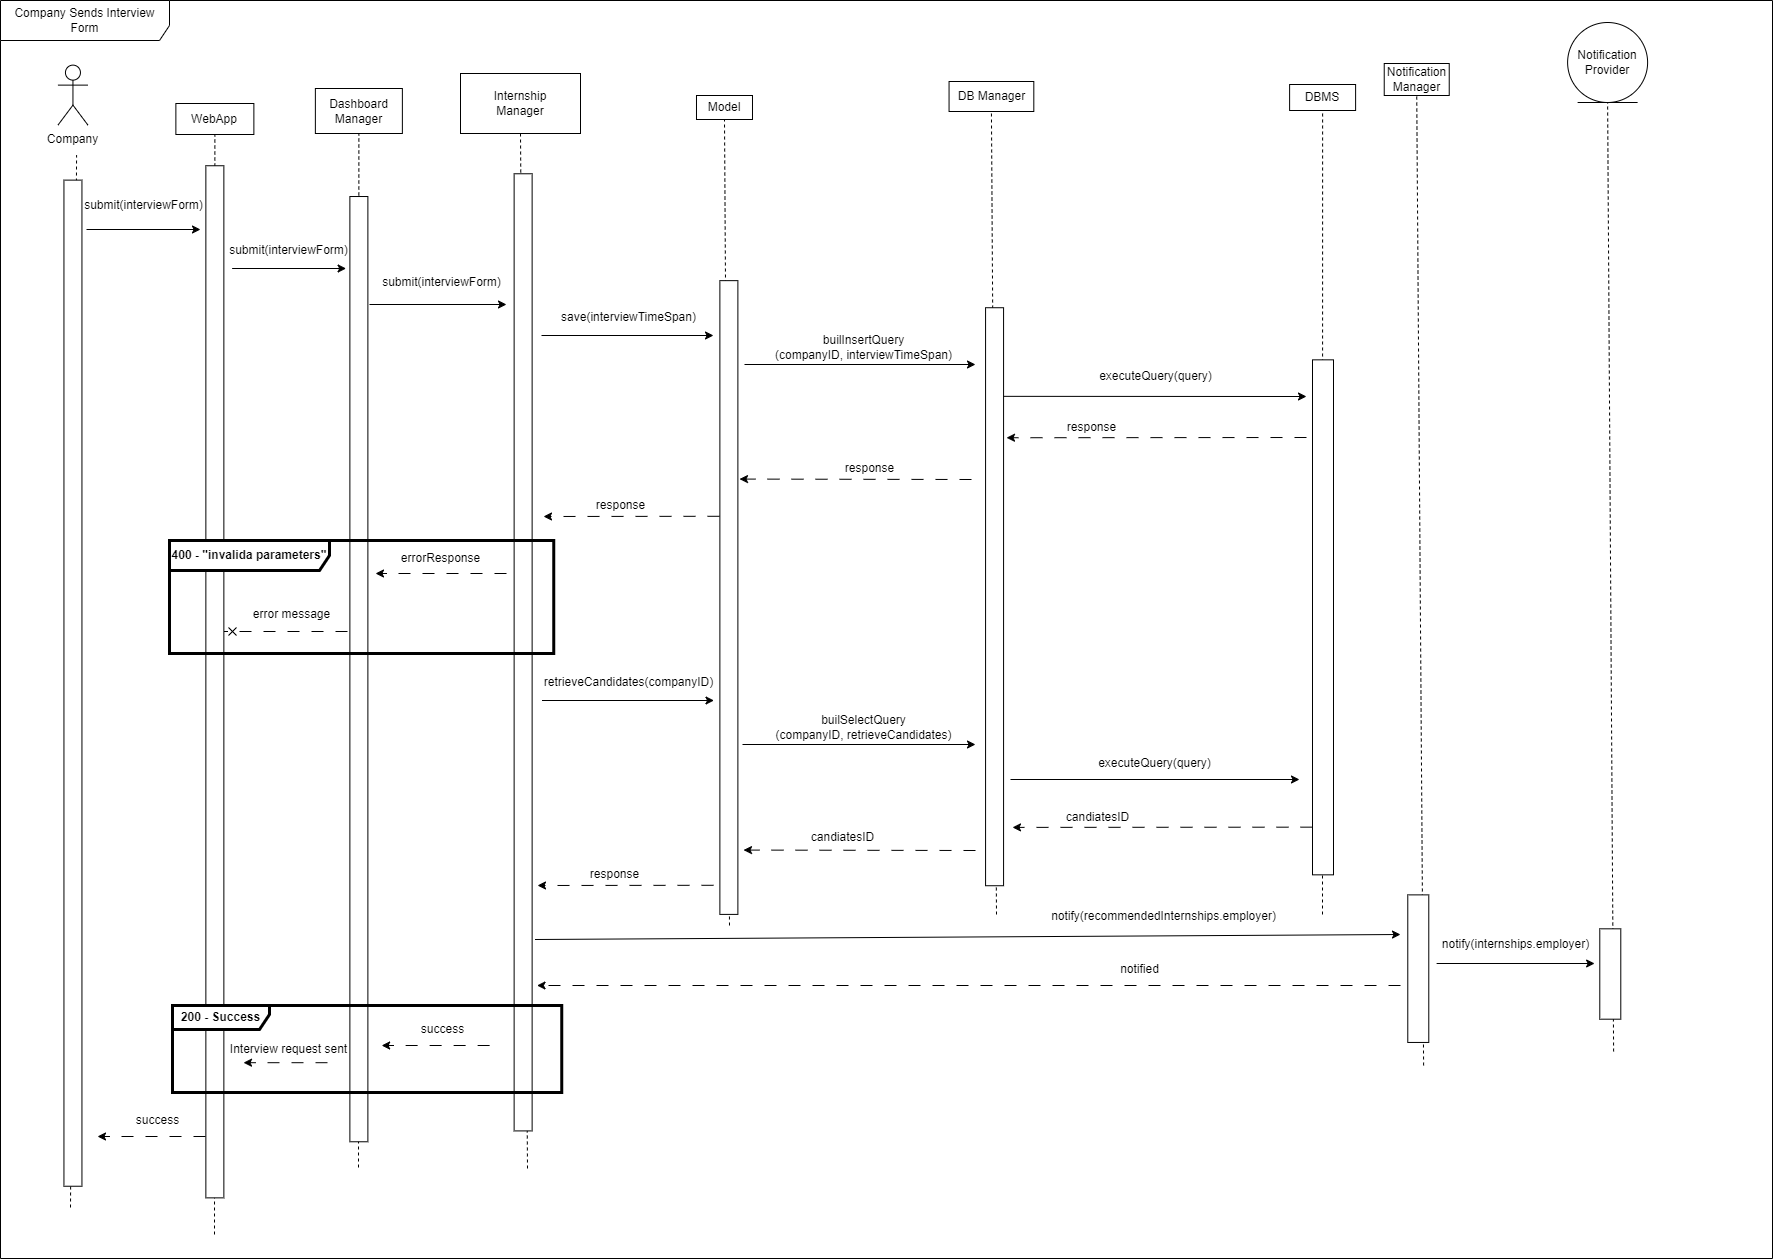
\includegraphics[scale = 0.25]{DD_figures/RuntimeView/CompanySendsInterviewFormRV.drawio.png}\\
\caption{Company Sends Interview Form}
\end{figure}

\newpage

\subsubsection*{Student Selects Interview Date}
The student submits a time slot form via the WebApp, which is then handled by the Internship Manager. This manager interacts with a Model component to save the student's ID, internship ID, and the chosen time slot. A database insert query is built and executed by the DB Manager, interacting with the DBMS Manager. The process can result in either a 400 error (invalid parameters) or a 200 success message. Upon success, the Internship Manager retrieves the company information associated with the internship from the database. This information is used by the Notification Manager to notify the company through a notification provider.
\begin{figure}[H]
\centering
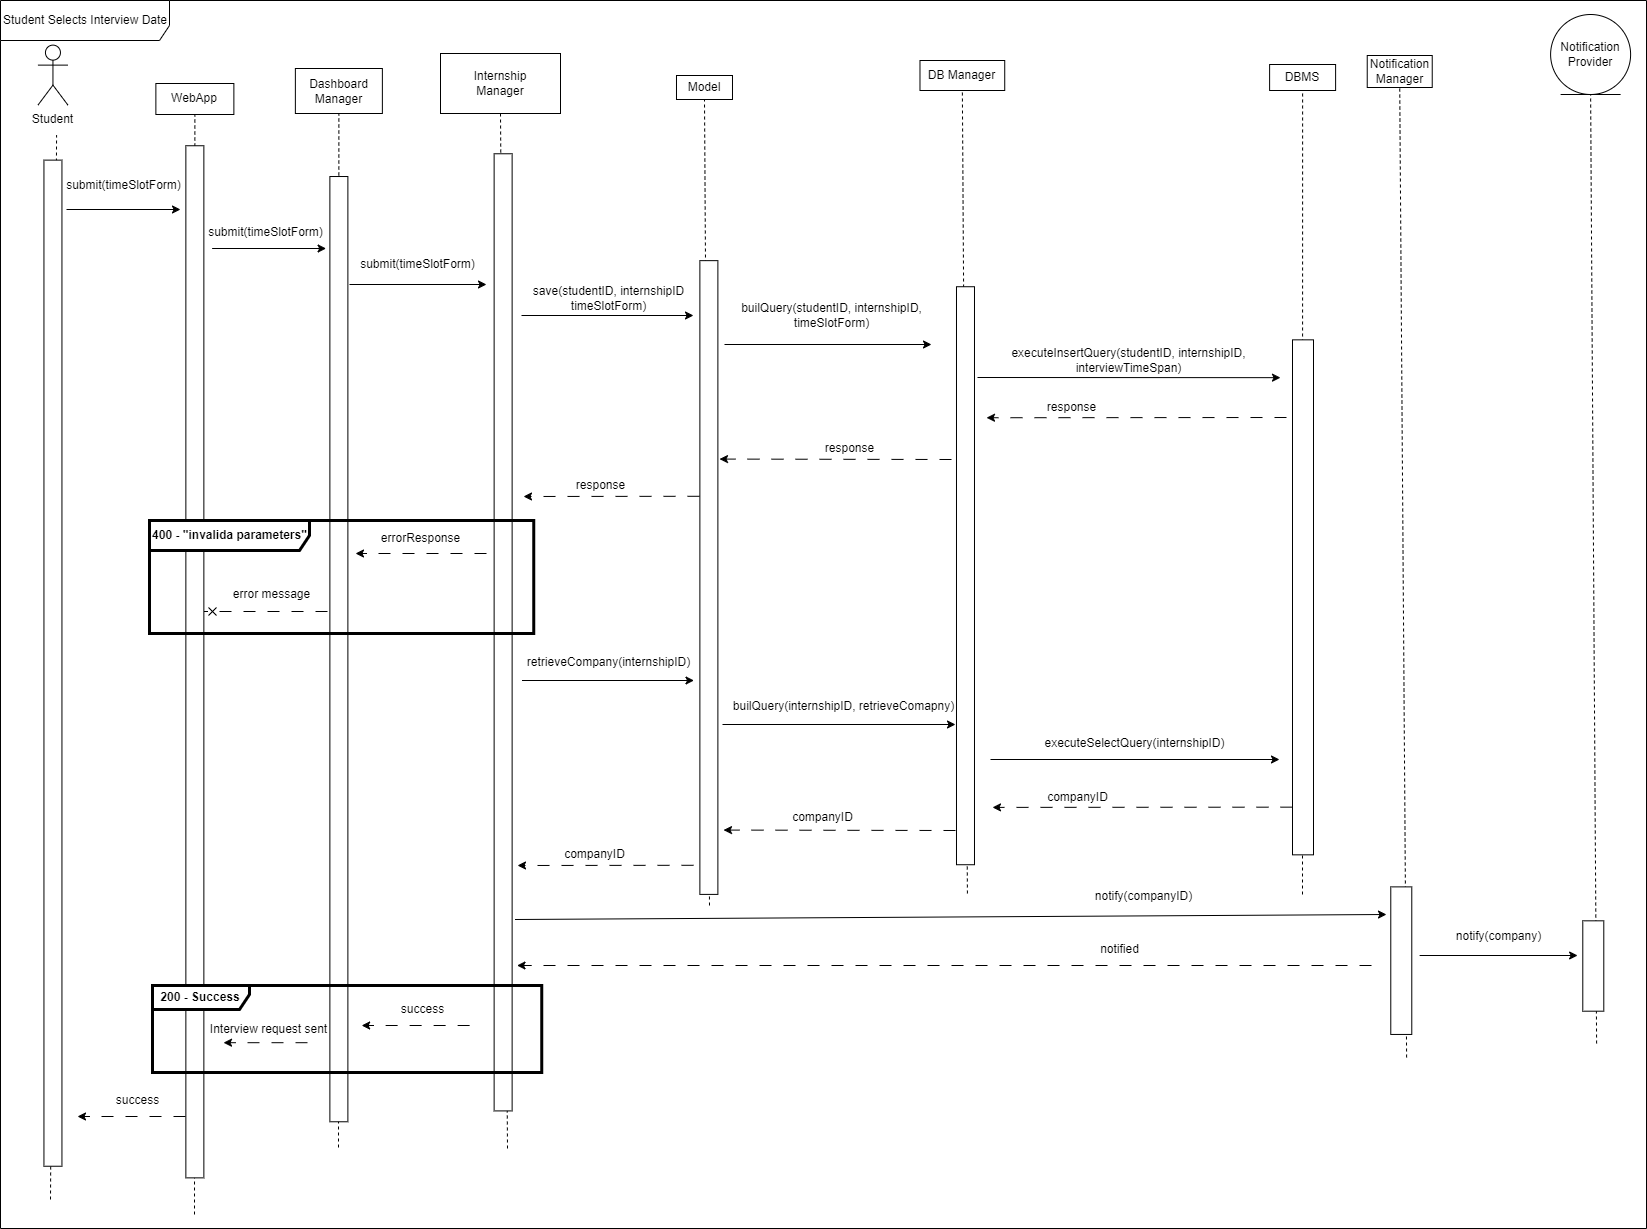
\includegraphics[scale = 0.25]{DD_figures/RuntimeView/StudentSelectsInterviewDateRV.drawio.png}\\
\caption{Student Selects Interview Date}
\end{figure}

\newpage
\subsubsection*{Company Selects Candidate}
The company sends a request containing the candidate ID and internship ID via the WebApp, which is received by the Internship Manager. This manager then uses a Model component to handle the data. A database insertion query is constructed and executed by the DB Manager, interacting with the DBMS. The process can result in a 400 error (invalid parameters) or a 200 success message. Upon successful candidate selection, the Internship Manager triggers a notification process. The Notification Manager then notifies the selected candidate through a notification provider.
\begin{figure}[H]
\centering
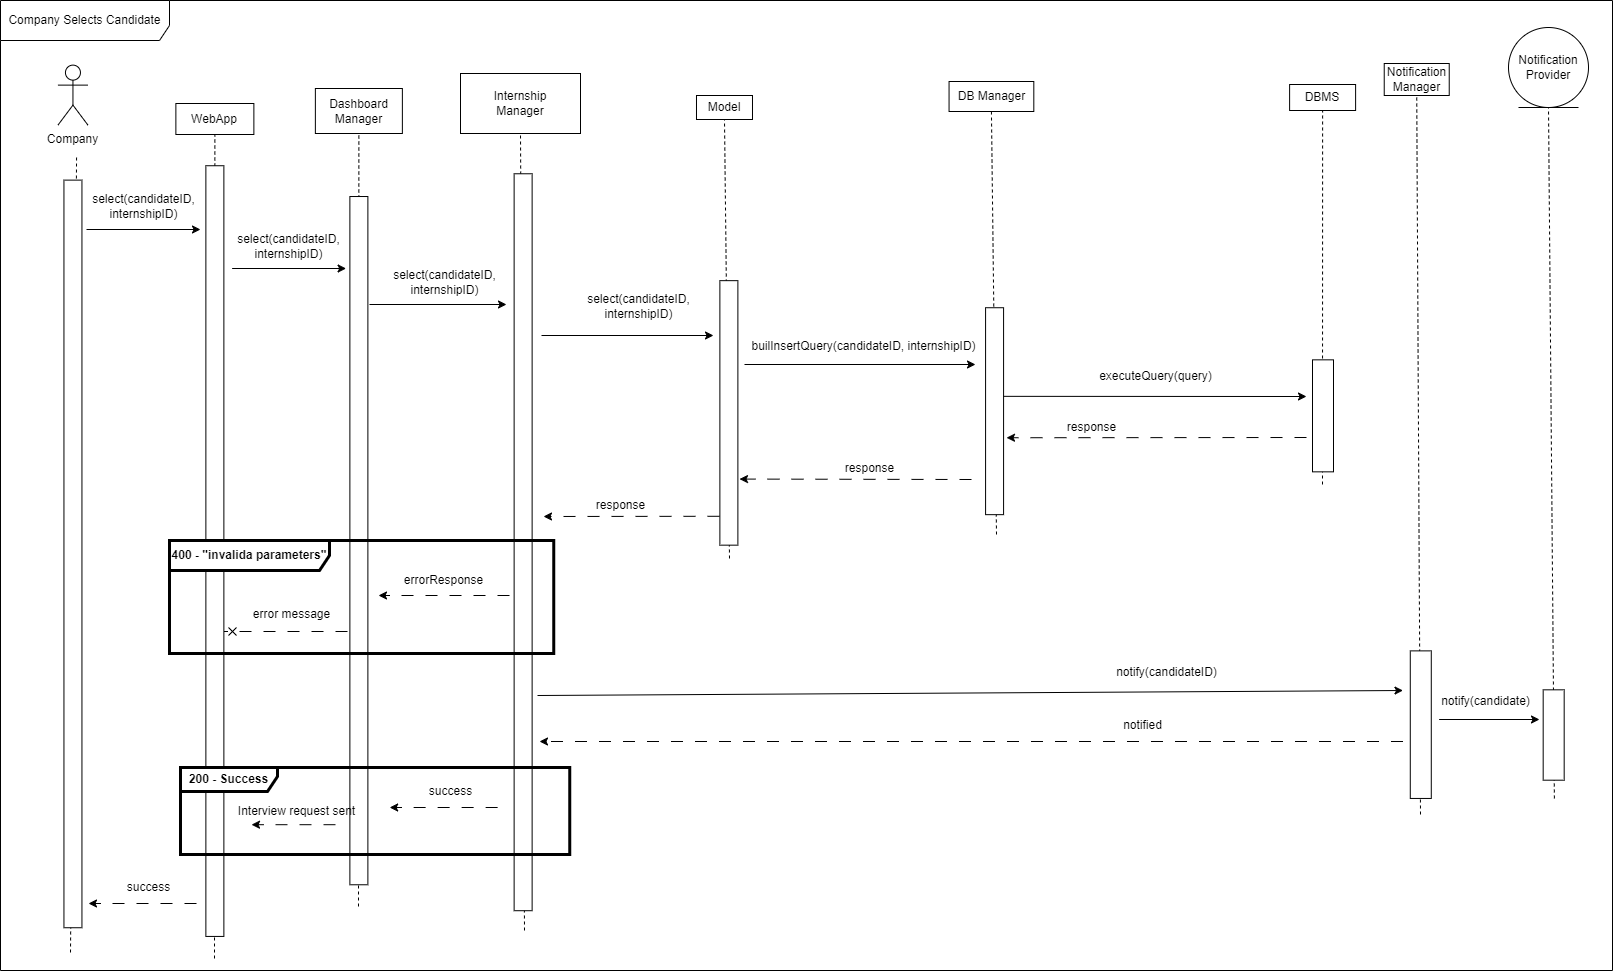
\includegraphics[scale = 0.30]{DD_figures/RuntimeView/CompanySelectsCandidateRV.drawio.png}\\
\caption{Company Selects Candidate}
\end{figure}

\newpage

\subsubsection*{Student Decides Offer}
This diagram illustrates the process by which a student responds to a company’s internship offer within the system. The sequence begins when the student navigates to the "Matched Internship" page from the "My Internship" page. The system retrieves the list of matched internships using the studentId through the relevant managers through the database and displays the results on the interface. Error-handling mechanisms ensure that only valid matches are presented, and if no matches are found, an error message is displayed to the user.
Only and only if an internship offer requires a response which shows in the alt section in the diagram, the system records the student’s decision in the database within a controlled loop to prevent potential errors. Upon acceptance, the advertisement status is updated, the changes are saved, and a notification is sent to the relevant company using the companyId and advertisementId parameters from the internship class. In the event of rejection, the advertisement is removed from the student's "Applied Positions" page. After processing the response, the system updates the interface, allowing the student to view the revised information while also preparing the database for the other related pages.
\begin{figure}[H]
\centering
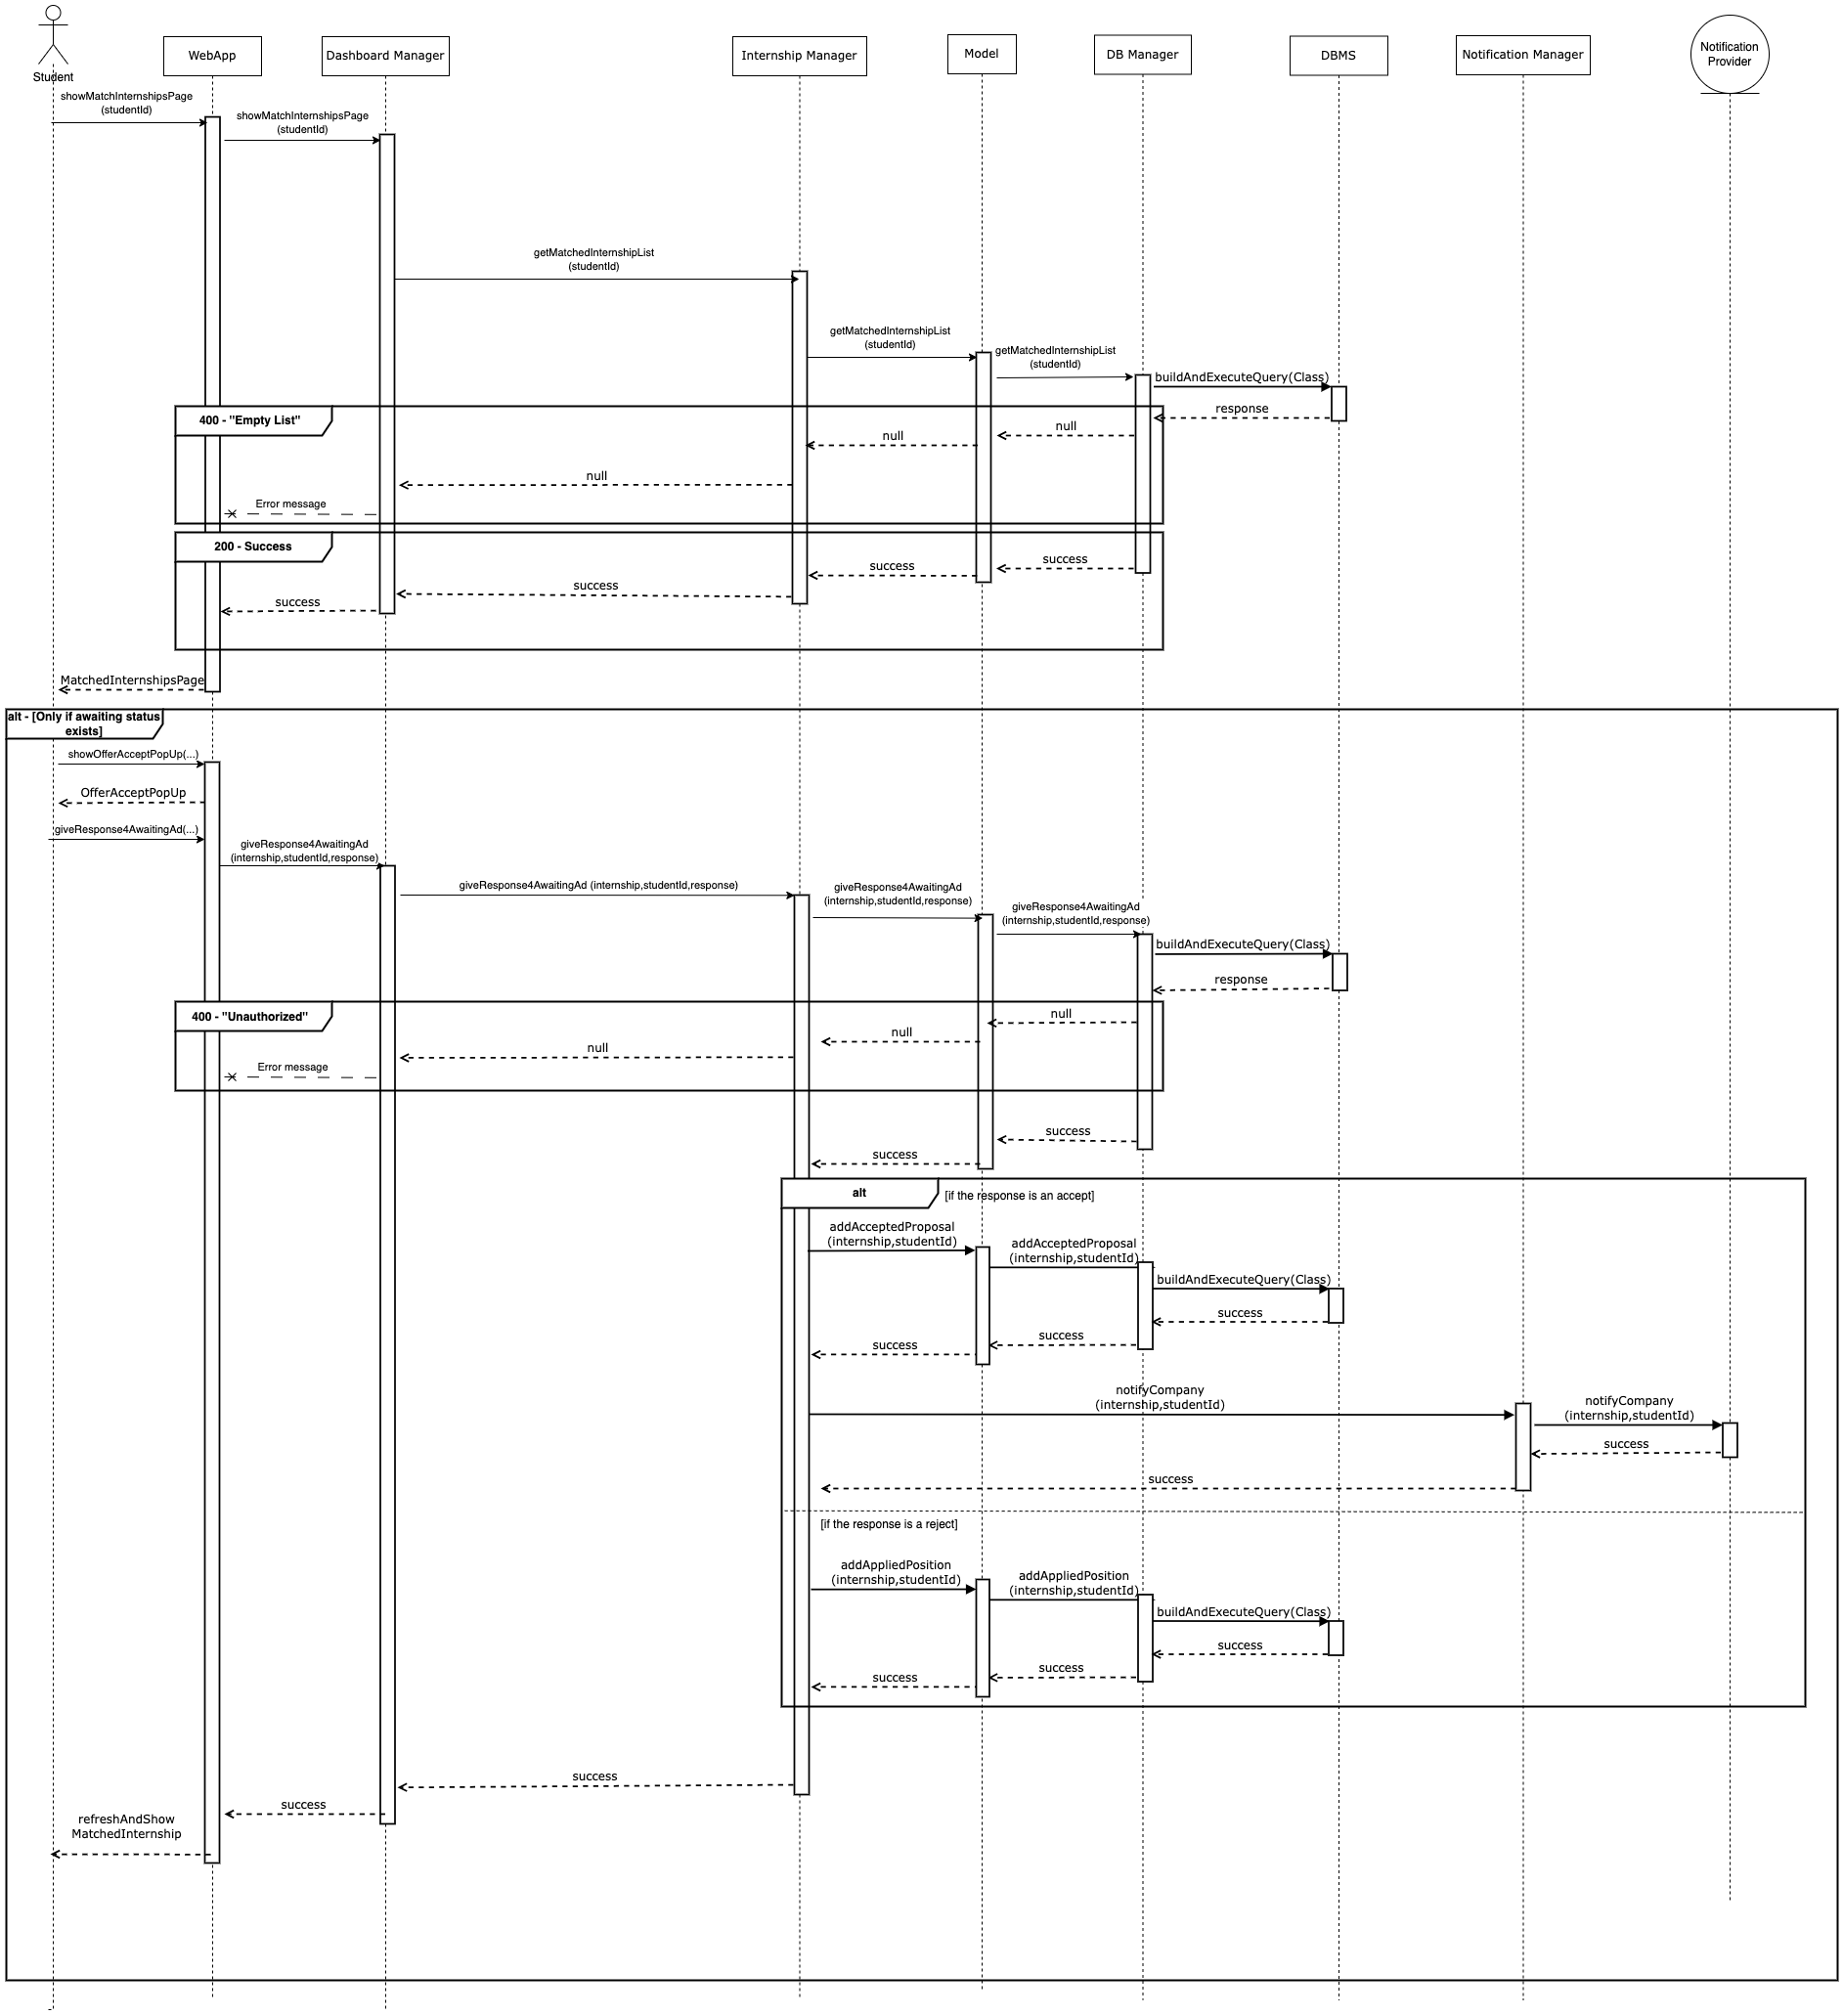
\includegraphics[scale = 0.15]{DD_figures/RuntimeView/studentConfirmCompany.drawio.png}
\caption{Student Accepts Or Rejects Internship}
\end{figure}
\newpage

\subsubsection*{User Views Comments}
The diagram below shows the process of a User visualizing comments of an internship. If the internshipID is not valid, the process is interrupted.
\begin{figure}[H]
\centering
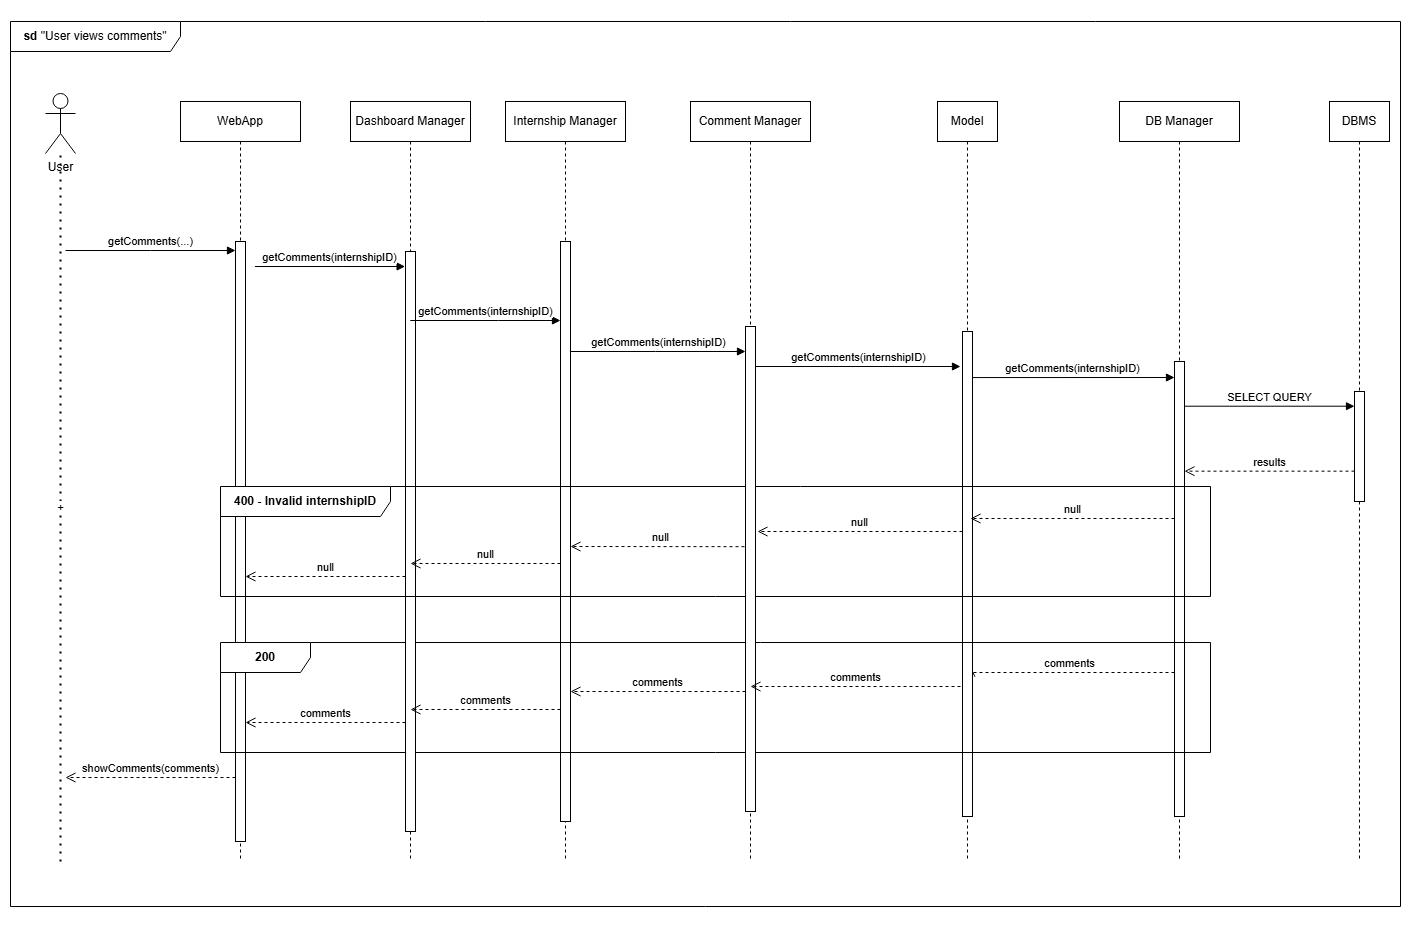
\includegraphics[scale = 0.4]{DD_figures/RuntimeView/UserViewsCommentsRV.png}\\
\caption{User Views Comments}
\end{figure}

\newpage

\subsubsection*{User Writes Observation}
The diagram below shows the process of a User (either student or company) writing an observation about an on-going internship. In this case no notifications are sent, which component will be important for the complaint part.
\begin{figure}[H]
\centering
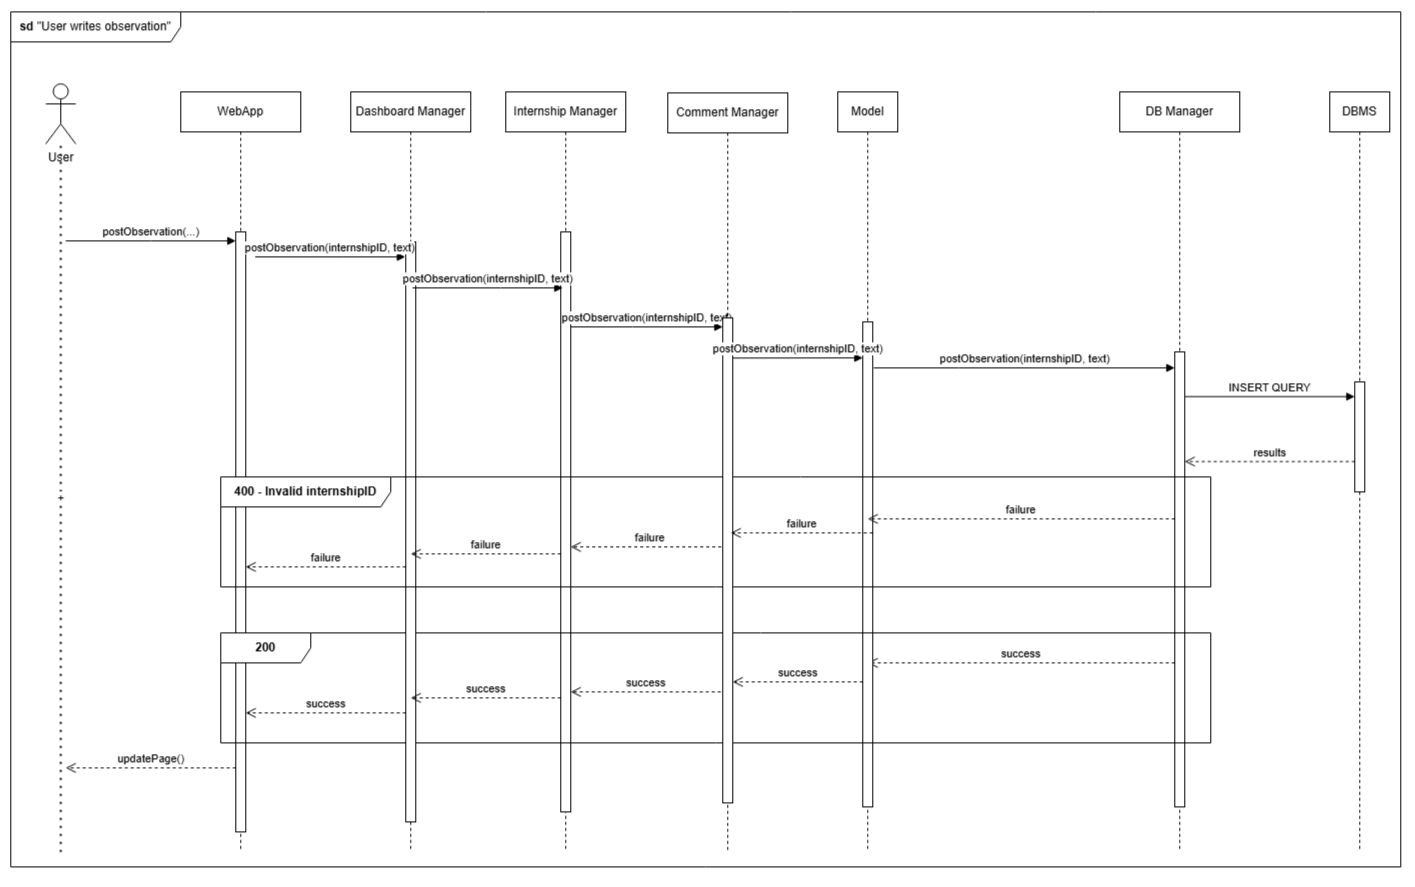
\includegraphics[scale = 0.4]{DD_figures/RuntimeView/UserWritesObservationRV.png}\\
\caption{User Writes Observation}
\end{figure}

\newpage

\subsubsection*{User Writes Complaint}
The diagram below shows the process of a User (either student or company) writing a complaint about an on-going internship. After the complaint has been posted successfully, the system will send a notification to the university of the student that is doing the internship, through the notification provider.
\begin{figure}[H]
\centering
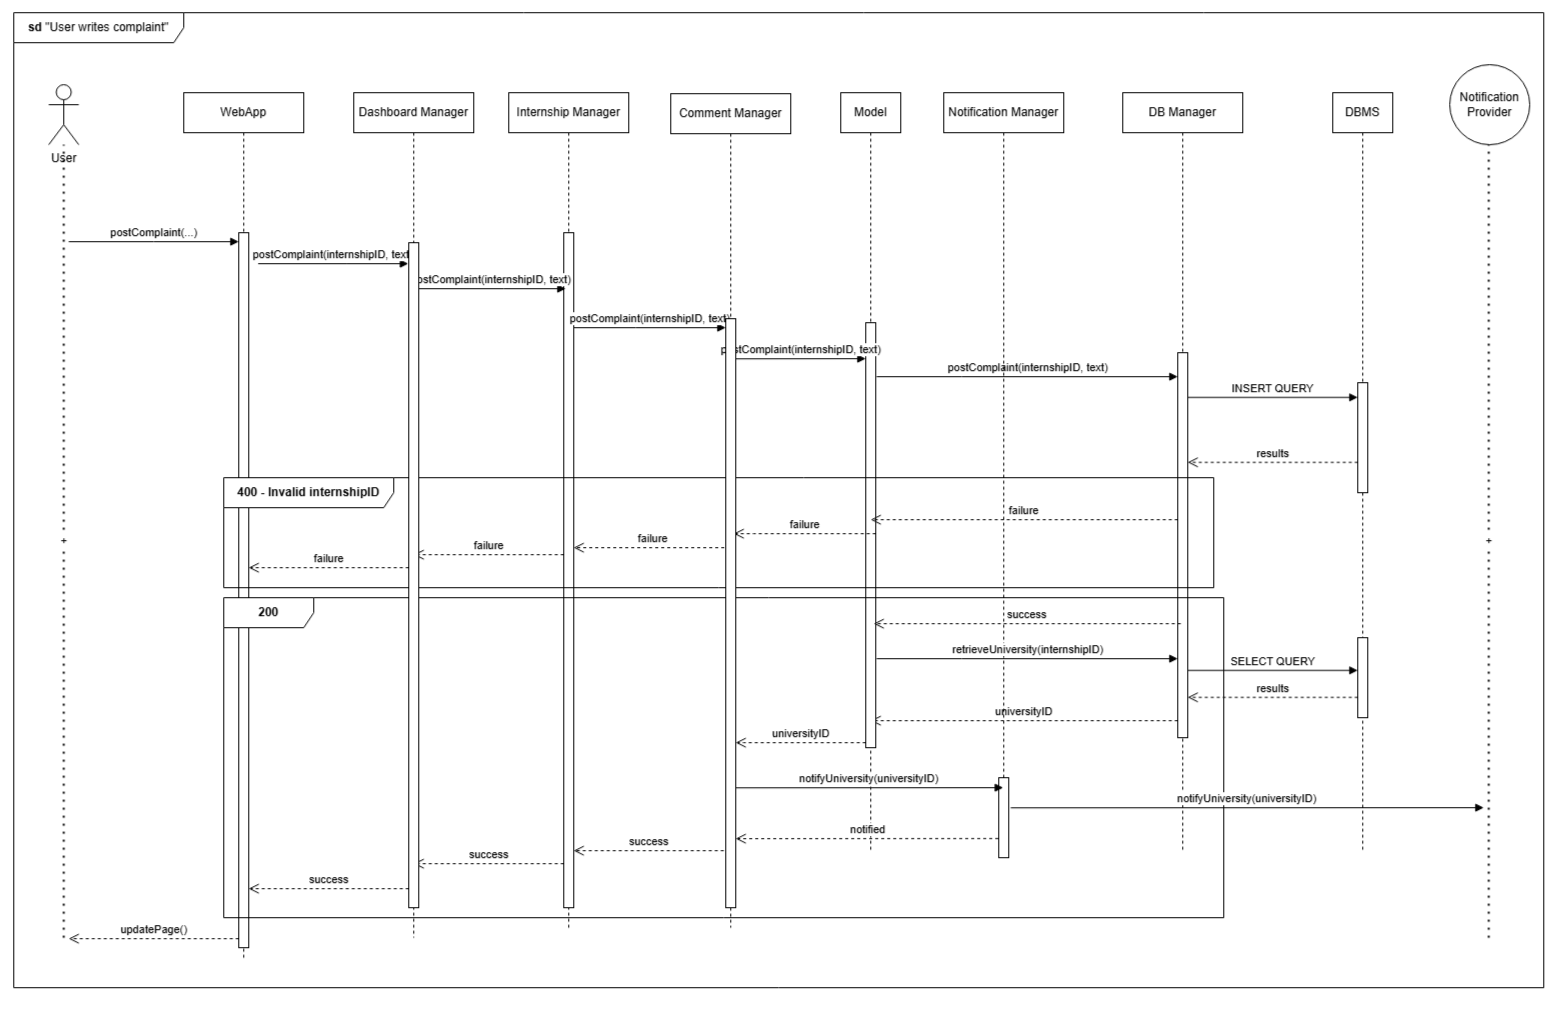
\includegraphics[scale = 0.4]{DD_figures/RuntimeView/UserWritesComplaintRV.png}\\
\caption{User Writes Complaint}
\end{figure}

\newpage

\subsubsection*{University Interrupts Internship}
The diagram below shows the process of a University interrupting an on-going internship. If the internshipID is not valid, the process interrupts. The platform will send notifications to the company and the student relative to that internship.
\begin{figure}[H]
\centering
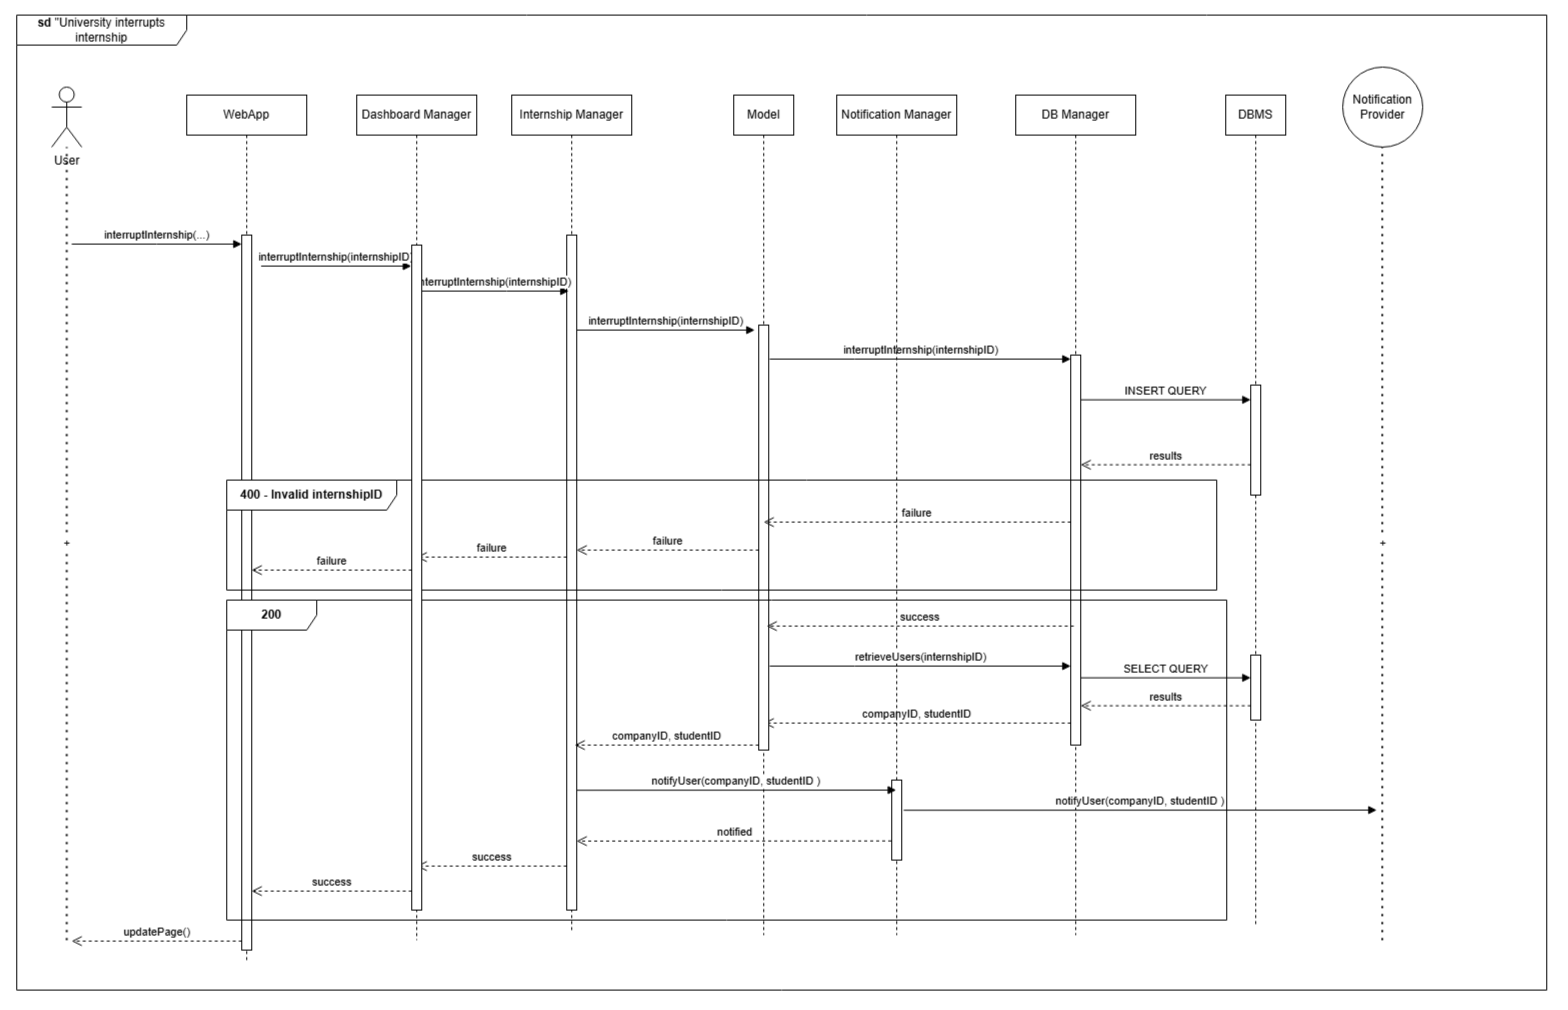
\includegraphics[scale = 0.4]{DD_figures/RuntimeView/UniversityInterruptsInternshipRV.png}\\
\caption{University Interrupts Internship}
\end{figure}

\newpage

\subsubsection*{ User Gives Feedback About The Experience}
The diagram shows that users must navigate to the "Accepted Proposal" page to provide feedback on their internship experience. Error-handling mechanisms, as in previous diagrams, ensure system security by addressing scenarios such as empty lists or unauthorized access. Functions utilizing the UserId parameter connect to the database through authorized managers, retrieving lists of accepted proposals or associated companies for display on the user interface. The mechanism within ''alt'' is designed to operate exclusively for cases that require feedback.Submitted responses are stored in the database, lists are updated via authorized managers, and the Interaction Manager processes the feedback for analysis. This interaction improves recommendation mechanism and helps to make it more correctly to the users, and finally the user interface is refreshed to reflect the updated status.
    \begin{figure}[H]
    \centering
    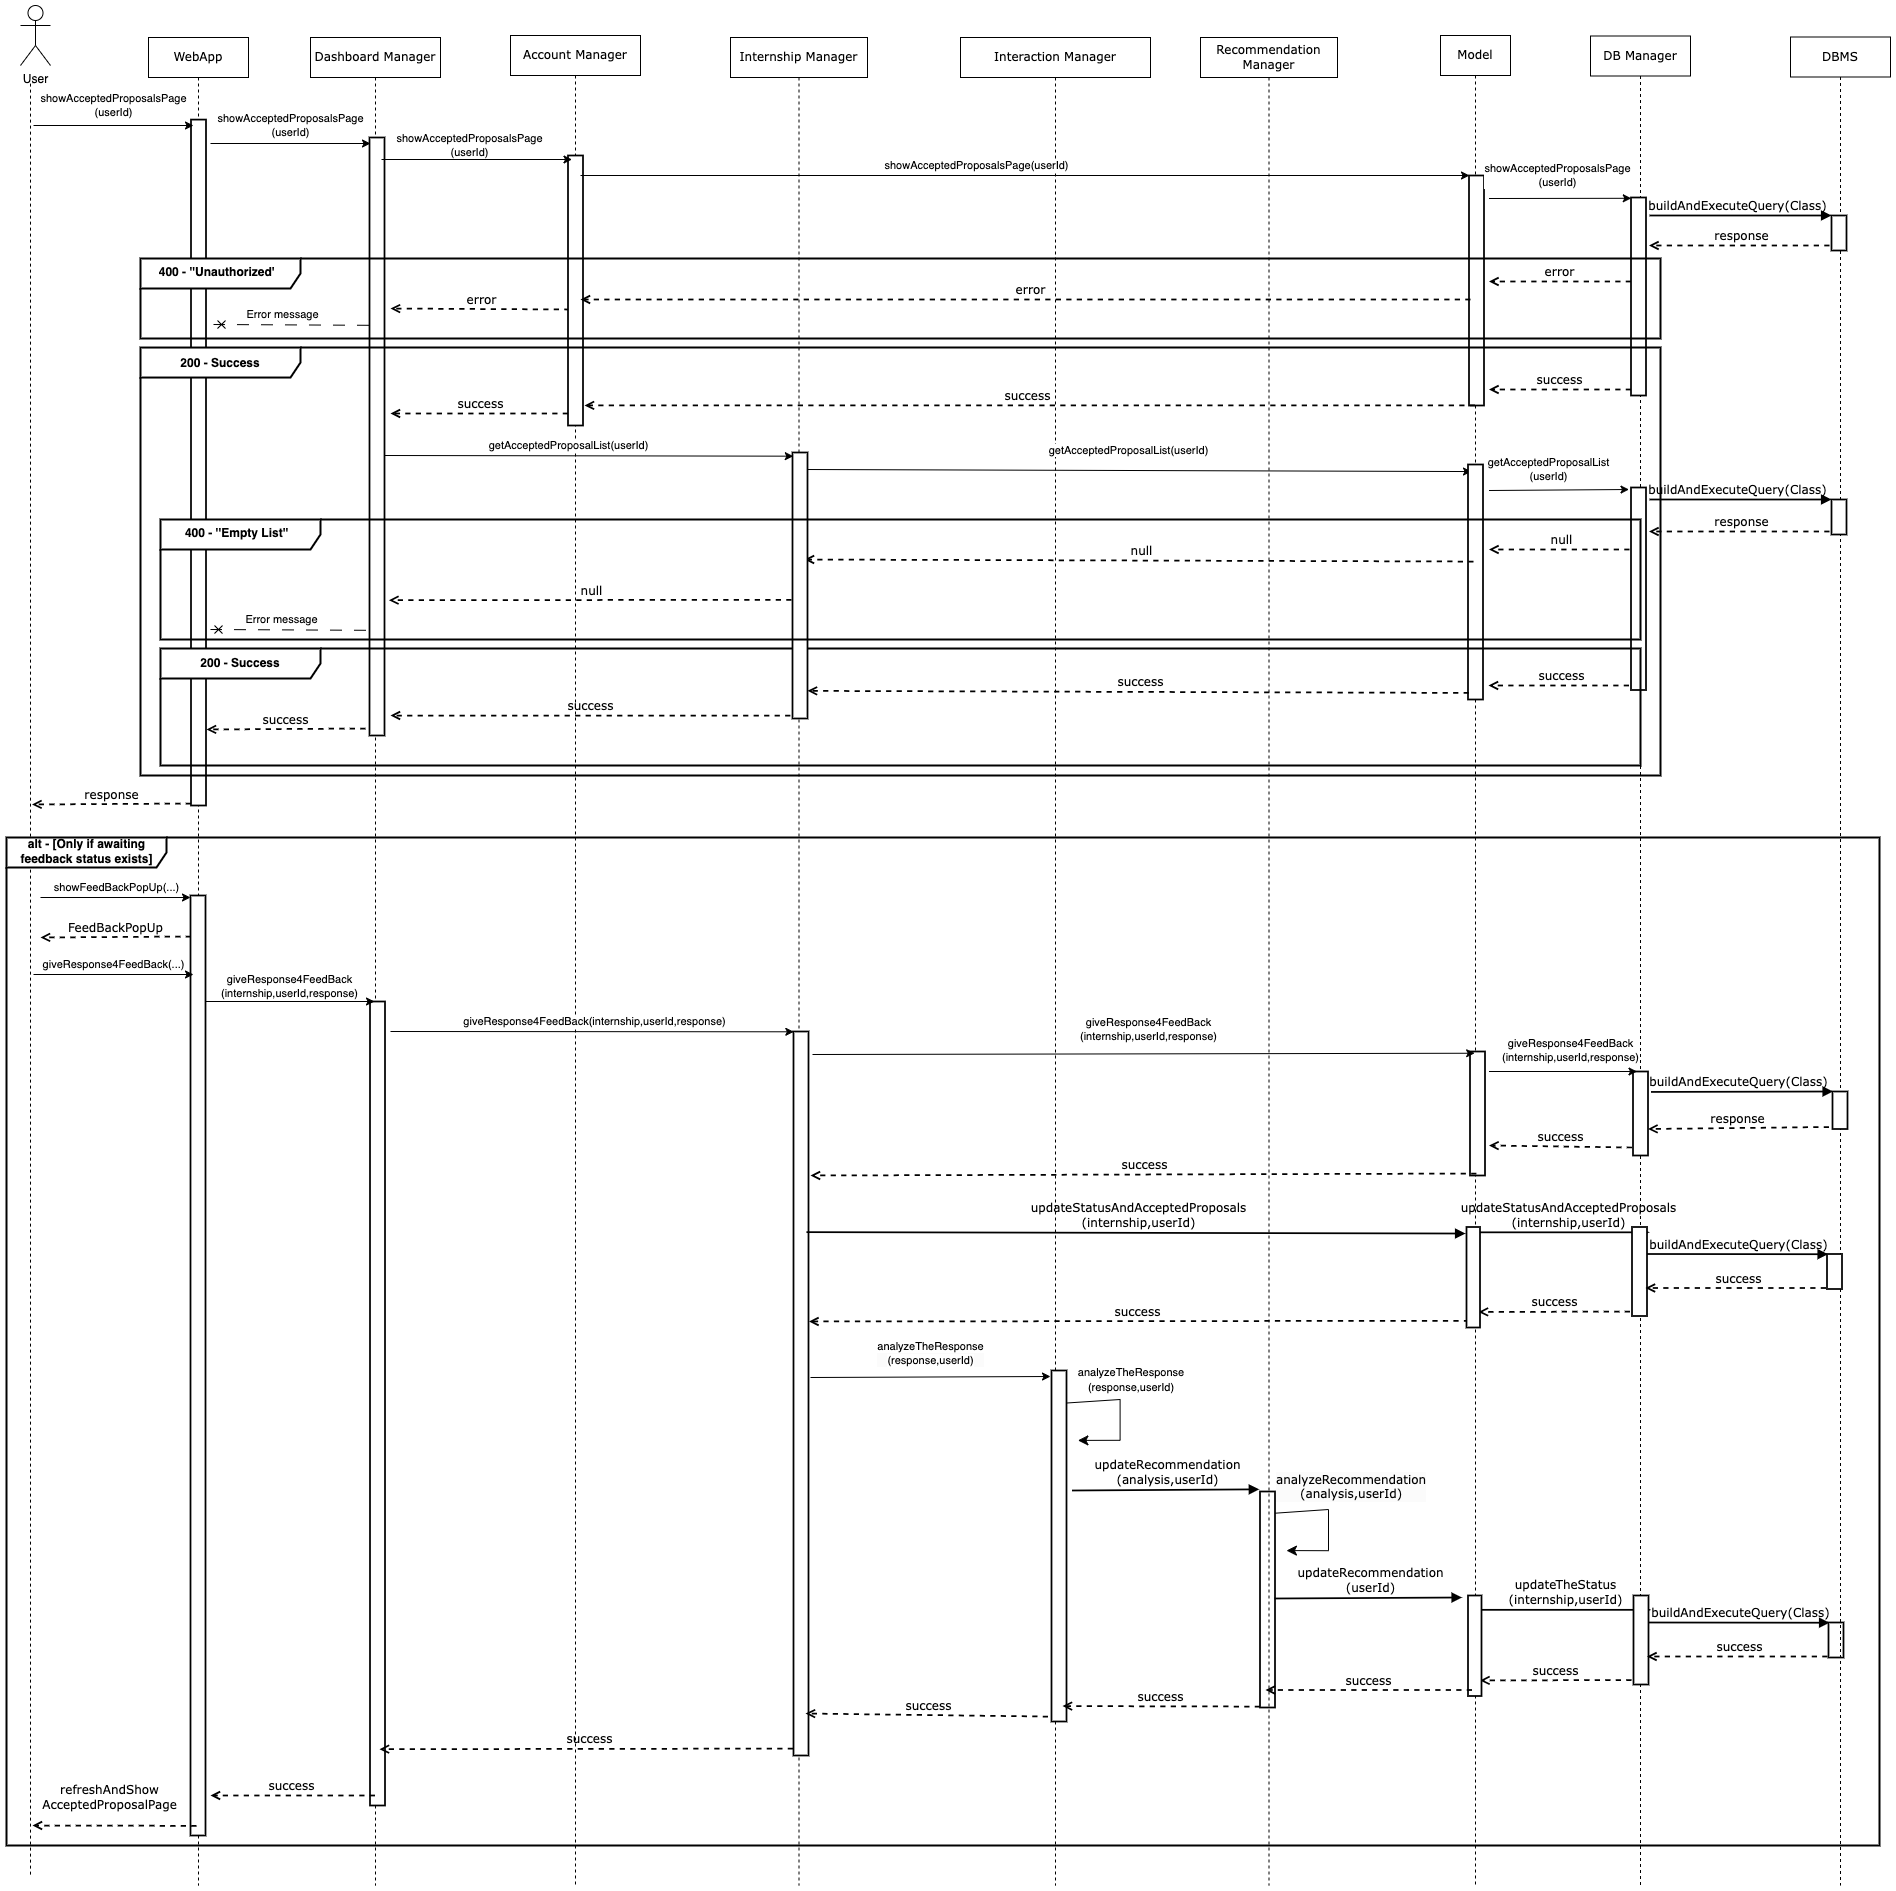
\includegraphics[scale = 0.22]{DD_figures/RuntimeView/userGivesFeedback.drawio.png}
    \caption{User Feedback}
\end{figure}




\subsection{Component Interfaces}
In this section, we use a class diagram to illustrate the component interfaces. The methods are presented as clearly as possible, and we expect their functionality to be easily understandable.
\begin{sidewaysfigure}
\centering
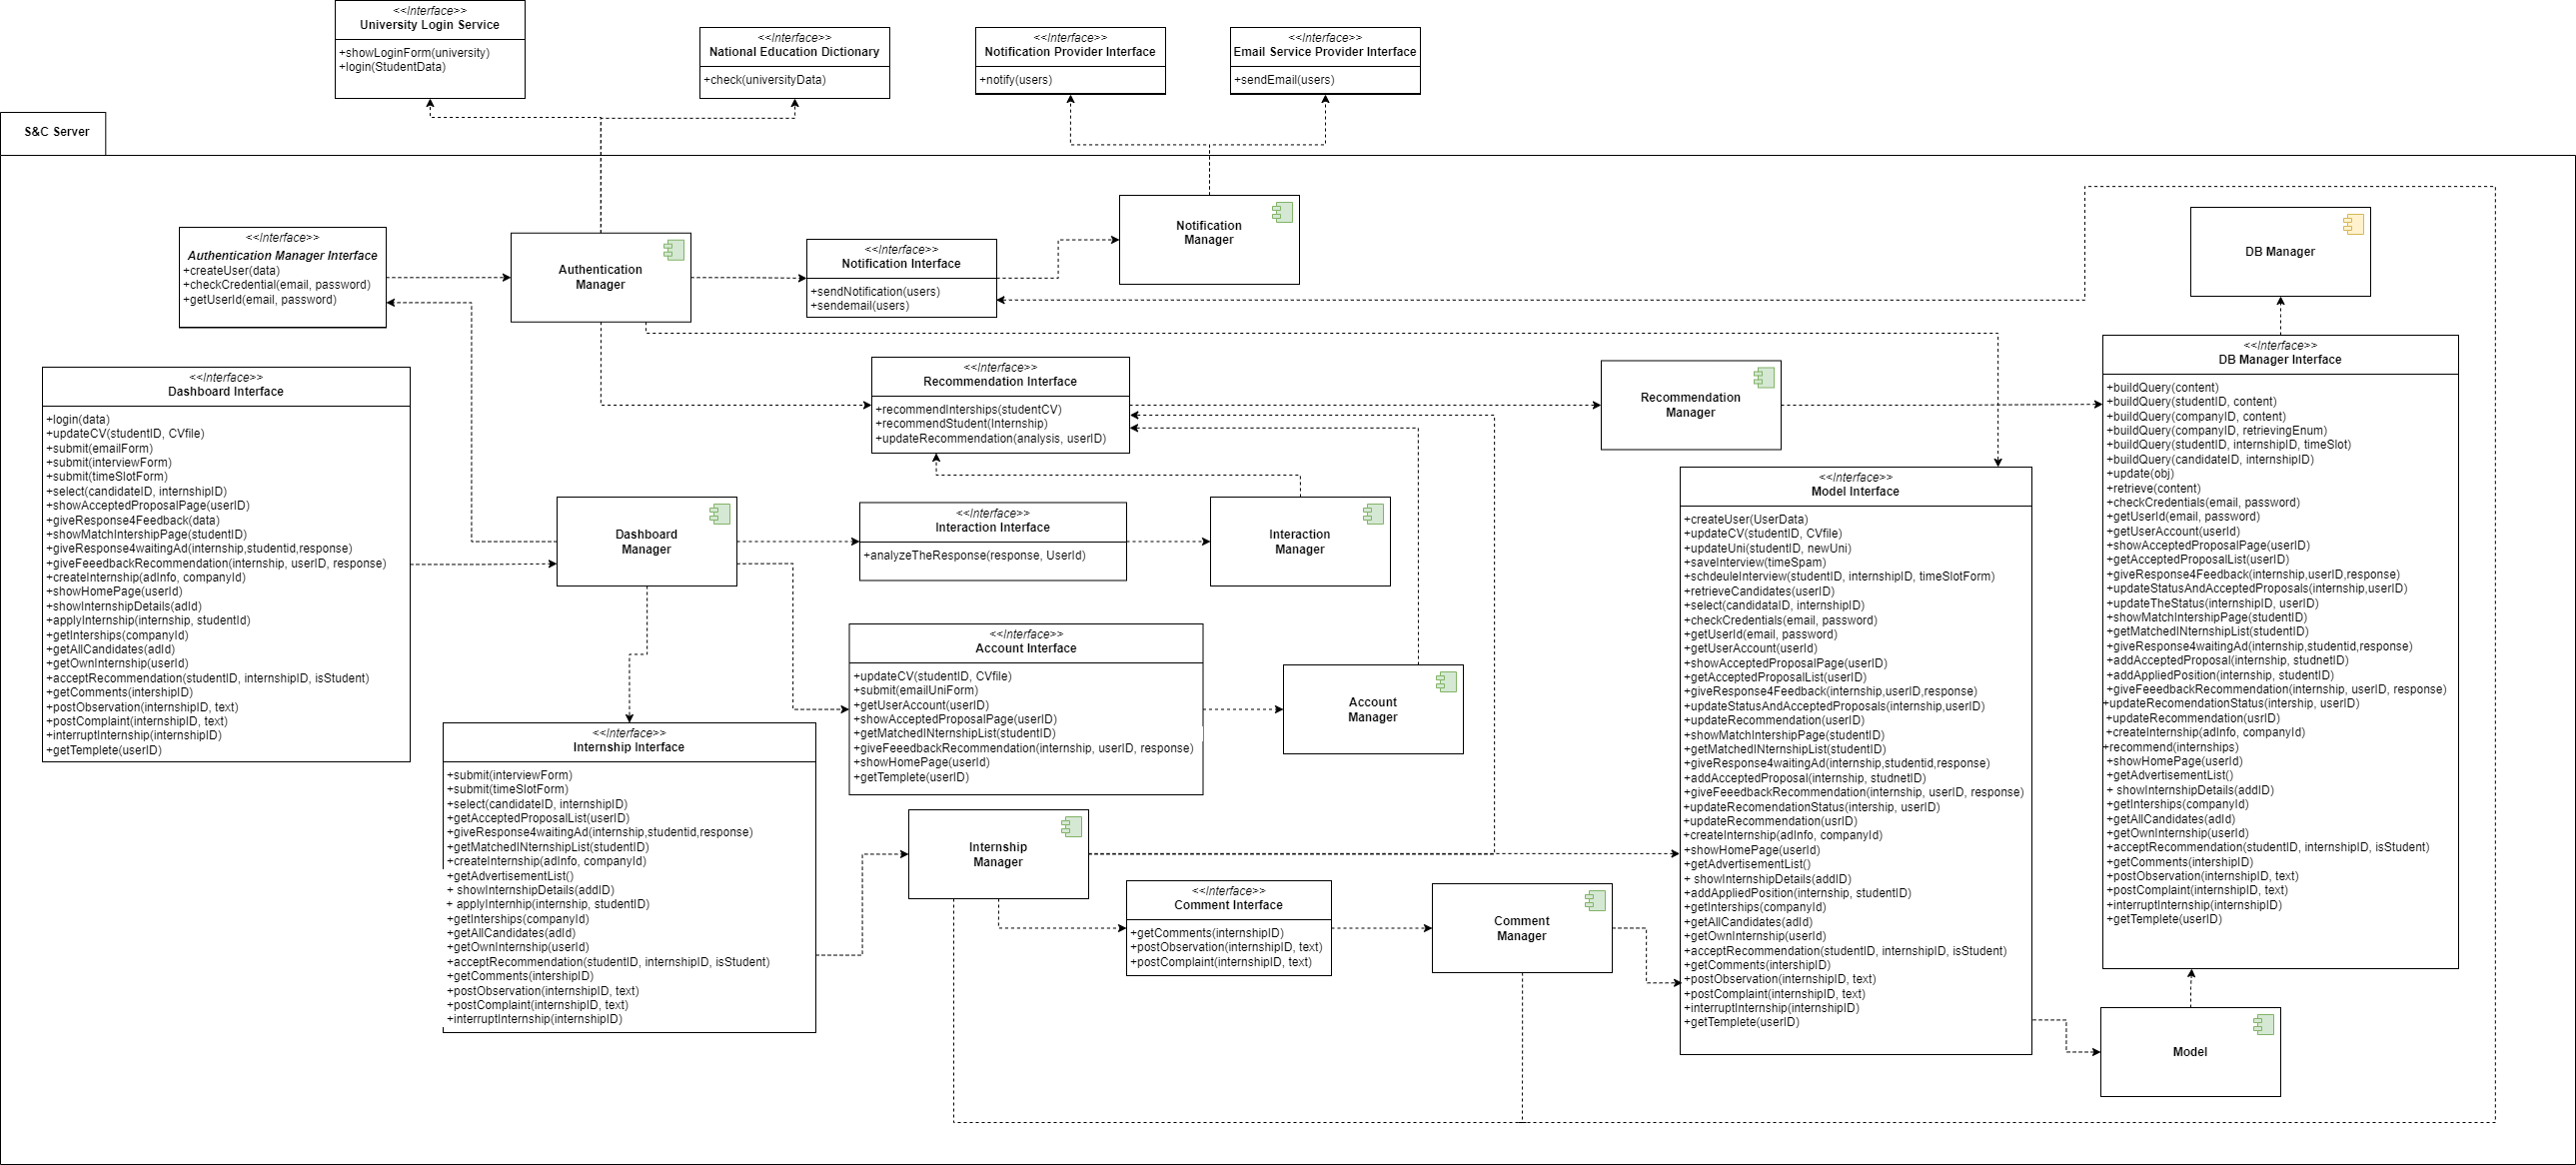
\includegraphics[scale = 0.30]{DD_figures/ComponentInterfaces.drawio.png}\\
\caption{Class diagram with interfaces of the S\&C System}
\end{sidewaysfigure}


\newpage
\subsubsection{API Endpoints}
In this section the API endpoints are presented. The focus is on the method used, on the parameters required and on the response.

\subsubsection*{POST api/users/register}
\begin{description}
    \item[Request Body:]  User: Object
    \item[200 Response:] message: String("User successfully registered") 
    \item[400 Response:] error : String("Invalid request data")
\end{description}

\subsubsection*{POST api/users/login}
\begin{description}
    \item[Request Body:]  User: Object
    \item[200 Response:] message: String("User successfully logged in") 
    \item[400 Response:] error : String("Invalid request data")
\end{description}

\subsubsection*{PUT api/student/\{studentId\}/updateCV}
\begin{description}
    \item[Request Body:]  CVfile: Object, studentId: int
    \item[200 Response:] message: String("CV successfully uploaded") 
    \item[400 Response:] error : String("Invalid request data")
\end{description}

\subsubsection*{PUT api/student/\{studentId\}/changeUni}
\begin{description}
    \item[Request Body:]  changeUni: emailUniForm, studentId: int
    \item[200 Response:] message: String("Student successfully changed university") 
    \item[400 Response:] error : String("Invalid parameters")
\end{description}

\subsubsection*{POST api/internship/create}
\begin{description}
    \item[Request Body:] adInfo: Object, companyId: int
    \item[200 Response:] message: String("Success") 
    \item[400 Response:] error : String("Invalid process")
\end{description}

\subsubsection*{GET api/internship}
\begin{description}
    \item[Request Body:]  userId: int
    \item[200 Response:] internships: Array of Object
    \item[400 Response:] error : String("Empty List")
\end{description}

\subsubsection*{GET api/internship/\{internshipId\}}
\begin{description}
    \item[200 Response:] internship: Object
    \item[400 Response:] error : String("Invalid data")
\end{description}

\subsubsection*{POST api/internship/\{internshipId\}/apply}
\begin{description}
    \item[Request Body:] studentId: int
    \item[200 Response:] message: String("Success")
    \item[400 Response:] error : String("Invalid data")
\end{description}

\subsubsection*{PUT api/student/\{studentId\}/appliedPosition}
\begin{description}
    \item[Request Body:] internship: Object
    \item[200 Response:] message: String("Success")
\end{description}

\subsubsection*{GET api/internship/created}
\begin{description}
    \item[Request Body:]  companyId: int
    \item[200 Response:] internships: Array of Object
    \item[400 Response:] error : String("Invalid data")
\end{description}

\subsubsection*{GET api/internship/allCandidates}
\begin{description}
    \item[Request Body:]  companyId: int, adId: int
    \item[200 Response:] allCandidates: Array of Object
    \item[400 Response:] error : String("Invalid data")
\end{description}

\subsubsection*{PUT api/internship/allCandidates}
\begin{description}
    \item[Request Body:] internship: Object, student: Object
    \item[200 Response:] message: String("Success")
\end{description}

\subsubsection*{GET api/internship/studentProfile}
\begin{description}
    \item[Request Body:]  student: Object, internship: Object
    \item[200 Response:] studentProfile: Object
    \item[400 Response:] error : String("Invalid data")
\end{description}

\subsubsection*{DELETE api/internship/removeFromAllCandidates}
\begin{description}
    \item[Request Body:] internship: Object, student: Object
    \item[200 Response:] message: String("Success")
\end{description}

\subsubsection*{DELETE api/internship/removeFromMatchedInternships}
\begin{description}
    \item[Request Body:] internship: Object, student: Object
    \item[200 Response:] message: String("Success")
\end{description}

\subsubsection*{DELETE api/internship/removeFromApprovedProfiles}
\begin{description}
    \item[Request Body:] internship: Object, student: Object
    \item[200 Response:] message: String("Success")
\end{description}

\subsubsection*{PUT api/company/approvedProfile}
\begin{description}
    \item[Request Body:] internship: Object, student: Object
    \item[200 Response:] message: String("Success")
\end{description}

\subsubsection*{POST api/user/acceptRecommendation}
\begin{description}
    \item[Request Body:] userId: int, internshipId: int
    \item[200 Response:] message: String("Success")
    \item[400 Response:] error : String("Invalid internshipId")
\end{description}

\subsubsection*{POST api/user/recommendationFeedback}
\begin{description}
    \item[Request Body:] feedback: Object, userId: int, internshipId: int
    \item[200 Response:] message: String("Success") 
    \item[400 Response:] error : String("Unauthorized")
\end{description}

\subsubsection*{PUT api/user/recommendations}
\begin{description}
    \item[Request Body:]  userId: int, internshipId: int
    \item[200 Response:] message: String("Success") 
\end{description}

\subsubsection*{POST api/internship/\{internshipId\}/interviews}
\begin{description}
    \item[Request Body:] interview: Object, studentId: int
    \item[200 Response:] message: String("Success") 
    \item[400 Response:] error : String("Invalid parameters")
\end{description}

\subsubsection*{POST api/internship/\{internshipId\}/timeSlot}
\begin{description}
    \item[Request Body:] timeSlot: time, studentId: int
    \item[200 Response:] message: String("Success") 
    \item[400 Response:] error : String("Invalid parameters")
\end{description}

\subsubsection*{POST api/internship/\{internshipId\}/selectsStudent}
\begin{description}
    \item[Request Body:] studentId: int
    \item[200 Response:] message: String("Success") 
    \item[400 Response:] error : String("Invalid parameters")
\end{description}

\subsubsection*{GET api/user/\{userId\}/acceptedProposals}
\begin{description}
    \item[200 Response:] acceptedProposals: Array of Objects 
    \item[400 Response:] error : String("Unauthorized")
\end{description}

\subsubsection*{GET api/user/\{userId\}/matchedInternships}
\begin{description}
    \item[200 Response:] matchedInternships: Array of Objects 
    \item[400 Response:] error : String("Empty List")
\end{description}

\subsubsection*{POST api/student/\{studentId\}/response}
\begin{description}
    \item[Request Body:] internship: Object, response: boolean
    \item[200 Response:] message: String("Success") 
    \item[500 Response:] error : String("Server side error")
\end{description}

\subsubsection*{PUT api/student/\{studentId\}/acceptedProposals}
\begin{description}
    \item[Request Body:] internship: Object
    \item[200 Response:] message: String("Success")
\end{description}

\subsubsection*{POST api/internship/\{internshipId\}/feedback}
\begin{description}
    \item[Request Body:] userId: int, response: boolean
    \item[200 Response:] message: String("Success") 
    \item[500 Response:] error : String("Server side error")
\end{description}

\subsubsection*{GET api/internship/\{internshipId\}/comments}
\begin{description}
    \item[Request Body:]  userId: int
    \item[200 Response:] comments: Array of Object 
    \item[400 Response:] error : String("Invalid internshipId")
\end{description}

\subsubsection*{POST api/internship/\{internshipId\}/comments}
\begin{description}
    \item[Request Body:]  userId: int
    \item[200 Response:] message: String("Success") 
    \item[400 Response:] error : String("Invalid internshipId")
\end{description}

\subsubsection*{POST api/internship/\{internshipId\}/observation}
\begin{description}
    \item[Request Body:] observation: Object, userId: int
    \item[200 Response:] message: String("Success") 
    \item[400 Response:] error : String("Invalid internshipId")
\end{description}

\subsubsection*{GET api/internship/\{internshipId\}/observations}
\begin{description}
    \item[Request Body:] userId: int
    \item[200 Response:] observations: Array of Object 
    \item[400 Response:] error : String("Invalid internshipId")
\end{description}

\subsubsection*{POST api/internship/\{internshipId\}/complaint}
\begin{description}
    \item[Request Body:] complaint: Object, internshipId: int
    \item[200 Response:] message: String("Success") 
    \item[400 Response:] error : String("Invalid internshipId")
\end{description}
\subsubsection*{GET api/internship/\{internshipId\}/complaints}
\begin{description}
    \item[Request Body:] userId: int
    \item[200 Response:] complaints: Array of Object
    \item[400 Response:] error : String("Invalid internshipId")
\end{description}

\subsubsection*{PUT api/internships/\{internshipId\}/interrupt}
\begin{description}
    \item[Request Body:] companyId: int, studentId: int
    \item[200 Response:] message: String("Success") 
    \item[400 Response:] error : String("Invalid internshipId")
\end{description}

\subsubsection*{GET api/user/\{userId\}/template}
\begin{description}
    \item[200 Response:] template: Object 
    \item[400 Response:] error : String("Invalid userId")
\end{description}


\newpage
\subsection{Selected Architectural Styles and Patterns}
\begin{itemize}
    \item \textbf{Three-Tier} The 3-tier architecture divides the system into three logical layers: presentation (Web Server), business logic (Application Server), and data storage (Database). It allows scalability, simplifies maintenance, and enhances control and security.

    \item \textbf{RESTful APIs} RESTful APIs (Representational State Transfer) follow a design paradigm based on specific principles for creating web services. They use standard HTTP methods (GET, POST, PUT, DELETE) and are stateless, allowing easy data exchange between systems. It provides seamless integration with various platforms and systems, it is simple to implement and reduces server load.

    \item \textbf{On-Cloud} The system is hosted on a cloud infrastructure, guaranteeing scalability and cost efficiency (all resources that are asked to the cloud provider are effectively used).
\end{itemize}

\subsection{Other Design Decisions}
\subsubsection{Database}
We selected a relational database for our system design because it is effective at storing structured data, enforcing data integrity, and providing fast query performance. In particular, we decided to use PostgreSQL, because it is open source and it is one of the most used relational databases.
\subsubsection{Distributed MVC Pattern}
This pattern divides the application into three
core components: Model, View, and Controller. The Model manages the data and business
logic, the View presents the data to users, and the Controller processes user input and system responses. This division allows simultaneous development of distinct parts of the system. The
distributed aspect of this pattern particularly aids in handling complex, scalable applications
by facilitating efficient data processing and user interface management across different systems
or networks.
\subsubsection{Interaction Manager}
We decided to implement a separate manager to take care of each interaction of the user with the system. In this first version the interaction are limited to feedback given by the users. However, if the recommendation mechanism needs to be modified in order to consider also other interactions of the users (e.g. logging viewing time and mouse movements), this is going to be possible through adaptation of the Interaction Manager.
\newpage

\section{User Interface Design}
This section presents the interface mockups, illustrating the operational flow of the system and the functionalities that will interact with the user. The system, which consists of three distinct primary interfaces designed based on user types (university, student, and company), is intended to be accessible on any desktop or mobile browser capable of facilitating user interaction.
\subsubsection*{Common Interfaces}
The system interface includes entrance, sign up, and sign in pages, which are commonly accessible regardless of user type. The mechanism within the system is structured according to user roles, such as universities, companies, or students, directing each type to the pages relevant to their specific functions.
\begin{figure}[H]
    \centering
    
\includegraphics[scale = 0.40]{figures/UserInterfaces/General/Entrance.png}
    \caption{Entrance}
    \centering
\end{figure}
\begin{figure}[H]
    \centering
    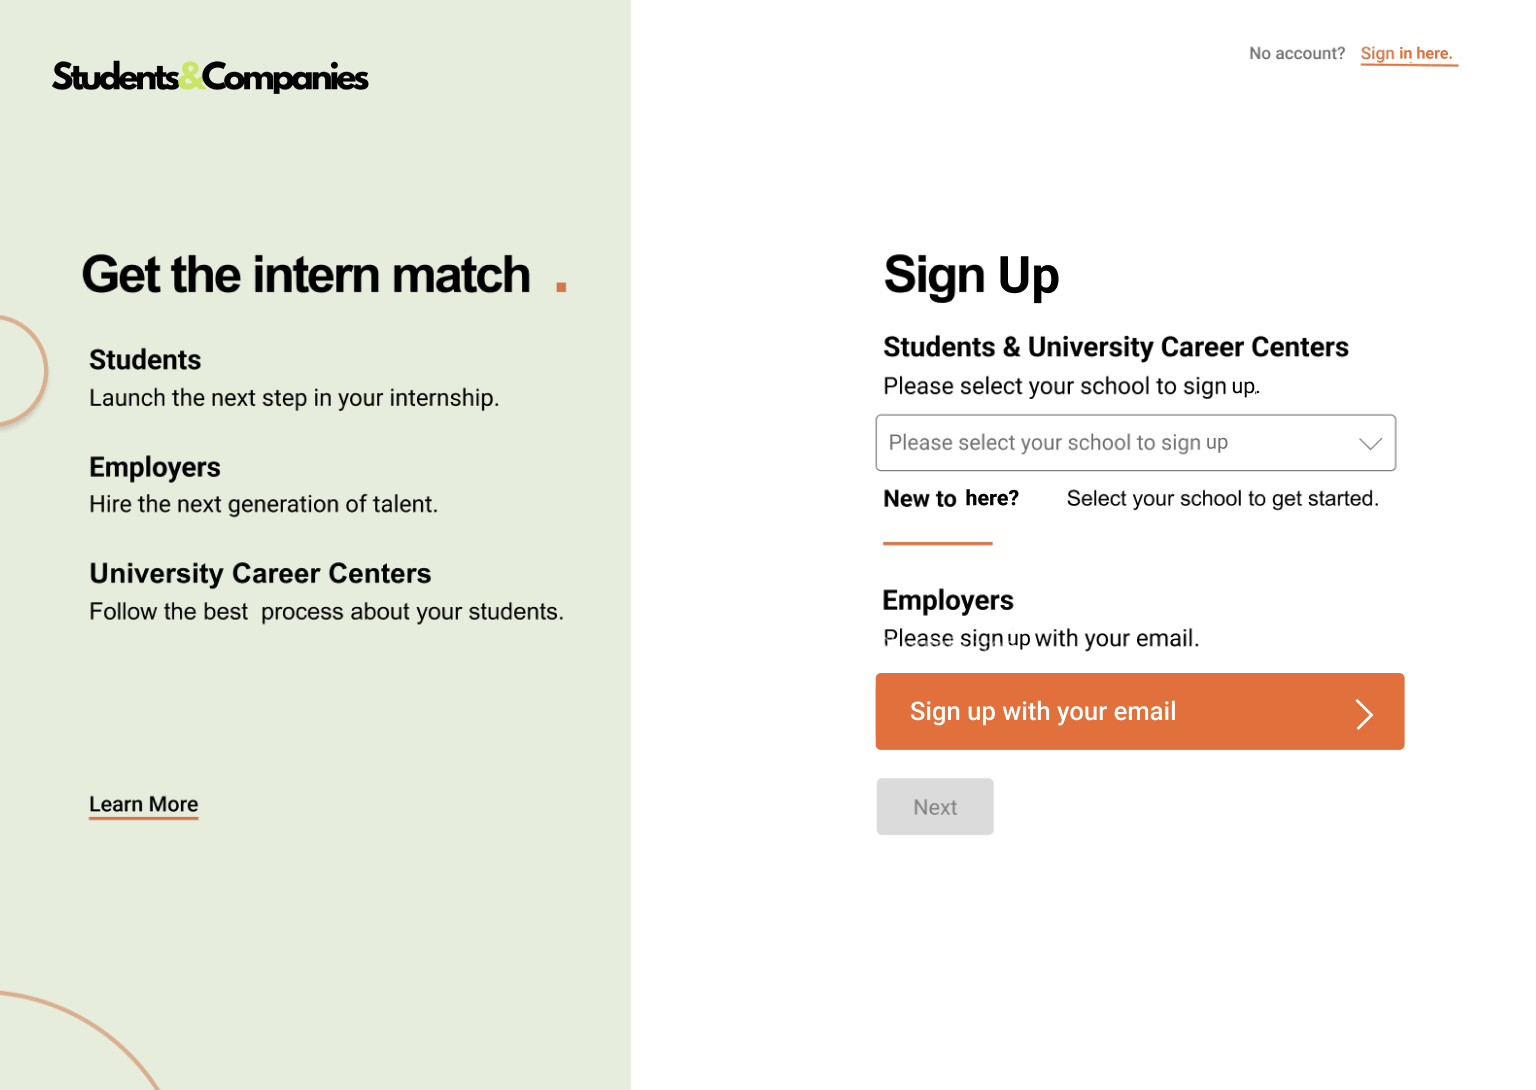
\includegraphics[scale = 0.40]{figures/UserInterfaces/General/HomeSignUp.png}
    \caption{Home Sign Up Page}
    \centering
\end{figure}
\begin{figure}[H]
    \centering
    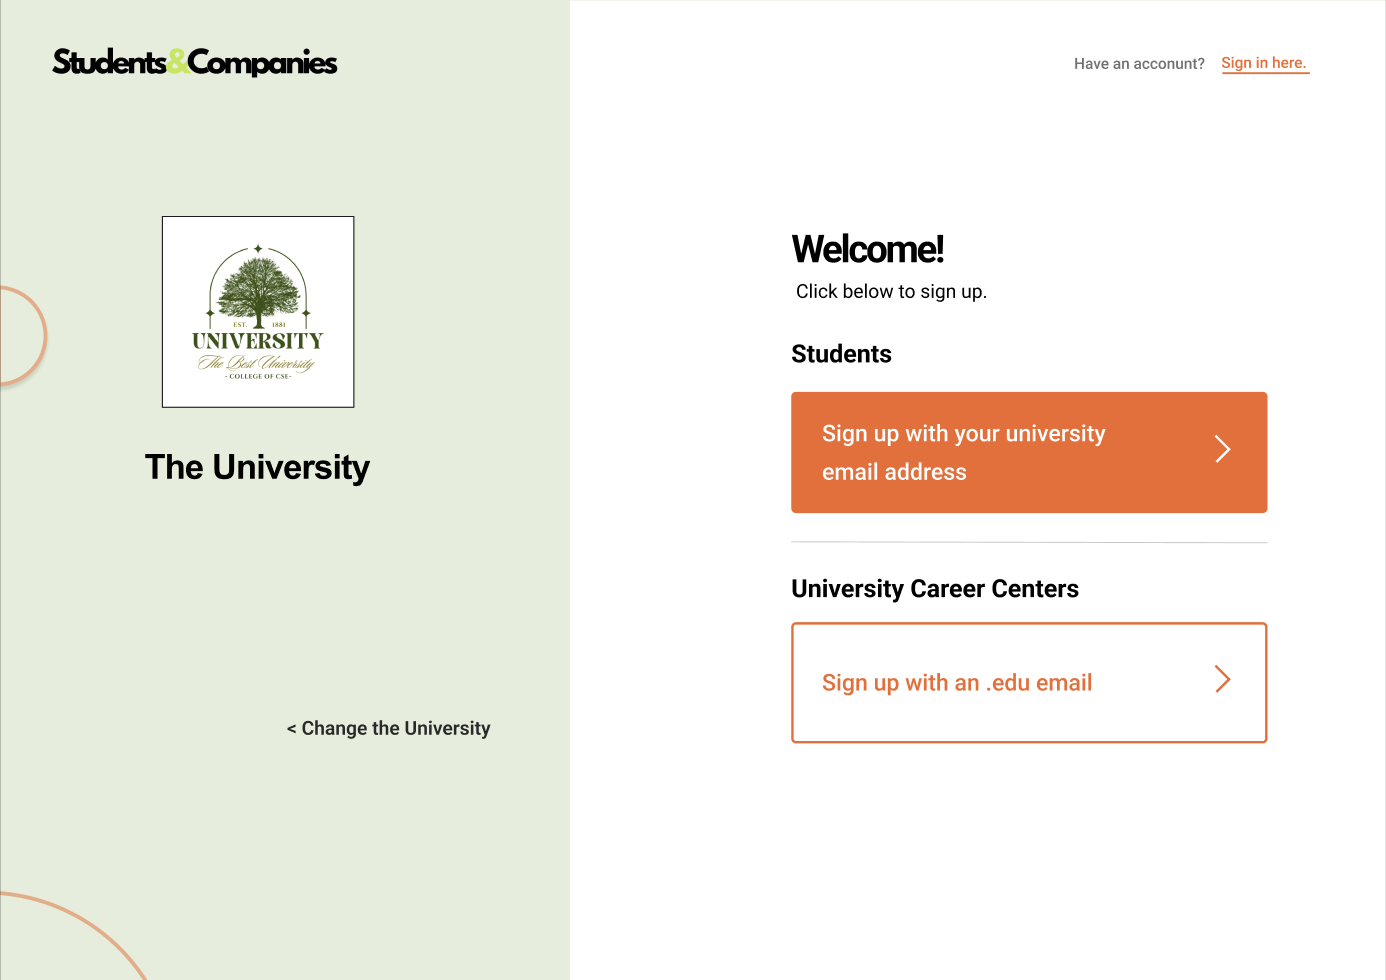
\includegraphics[scale = 0.45]{figures/UserInterfaces/General/SUSignUp.png}
    \caption{Student \& University Sign Up}
    \centering
\end{figure}

\begin{figure}[H]
    \centering
    
\includegraphics[scale = 0.45]{figures/UserInterfaces/General/StudentSignUp.png}
    \caption{Student Sign Up Page}
    \centering
\end{figure}
\begin{figure}[H]
    \centering
    
\includegraphics[scale = 0.42]{figures/UserInterfaces/General/StudentUploadCV.png}
    \caption{Student Upload CV}
    \centering
\end{figure}
\begin{figure}[H]
    \centering
    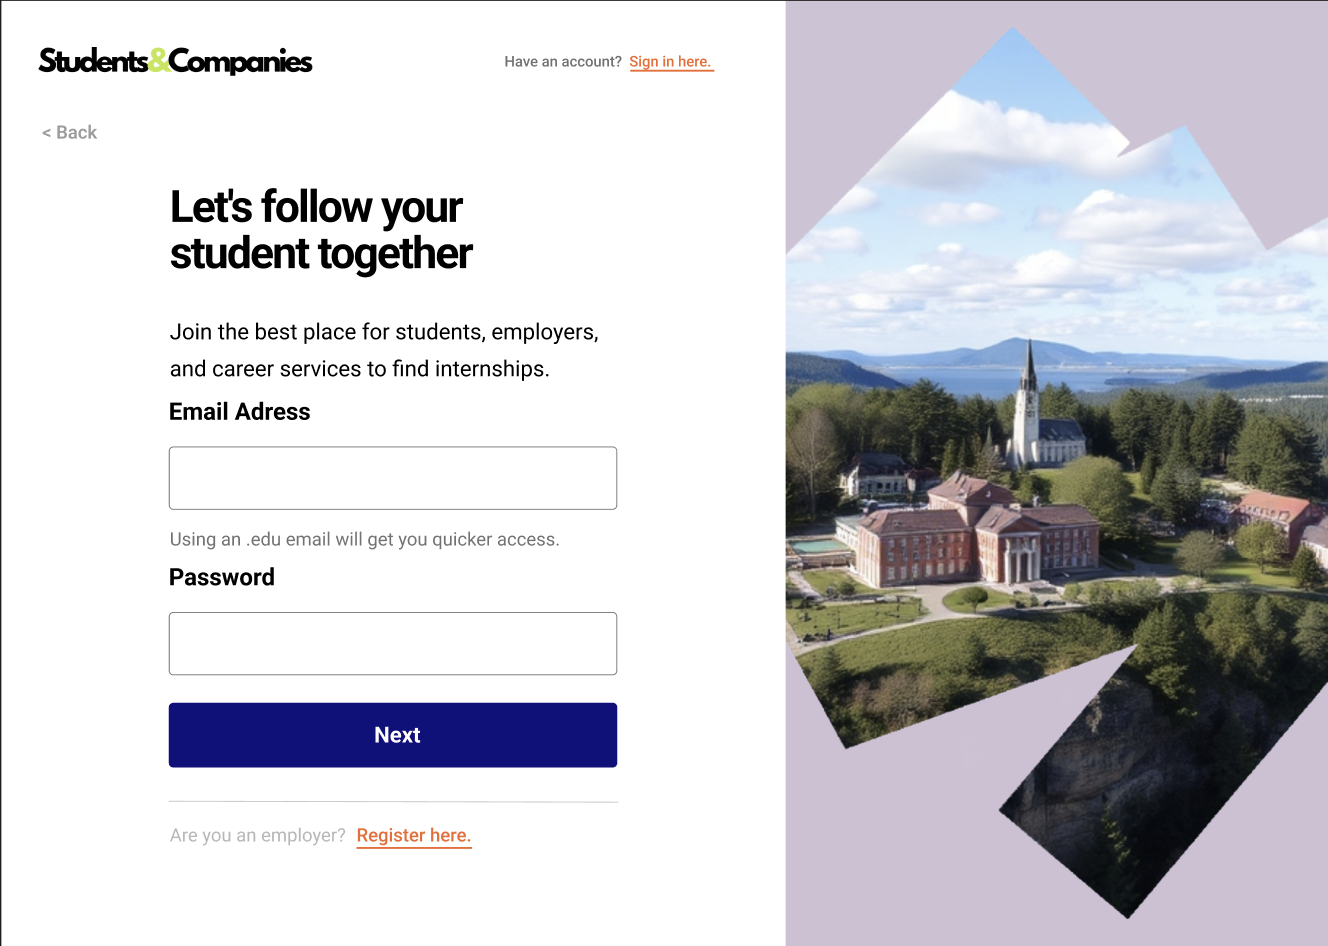
\includegraphics[scale = 0.45]{figures/UserInterfaces/General/UniversitySignUp.png}
    \caption{University Sign Up Page}
    \centering
\end{figure}
\begin{figure}[H]
    \centering
    
\includegraphics[scale = 0.45]{figures/UserInterfaces/General/EmployerSignUp.png}
    \caption{Employer Sign Up Page}
    \centering
\end{figure}

\begin{figure}[H]
    \centering
    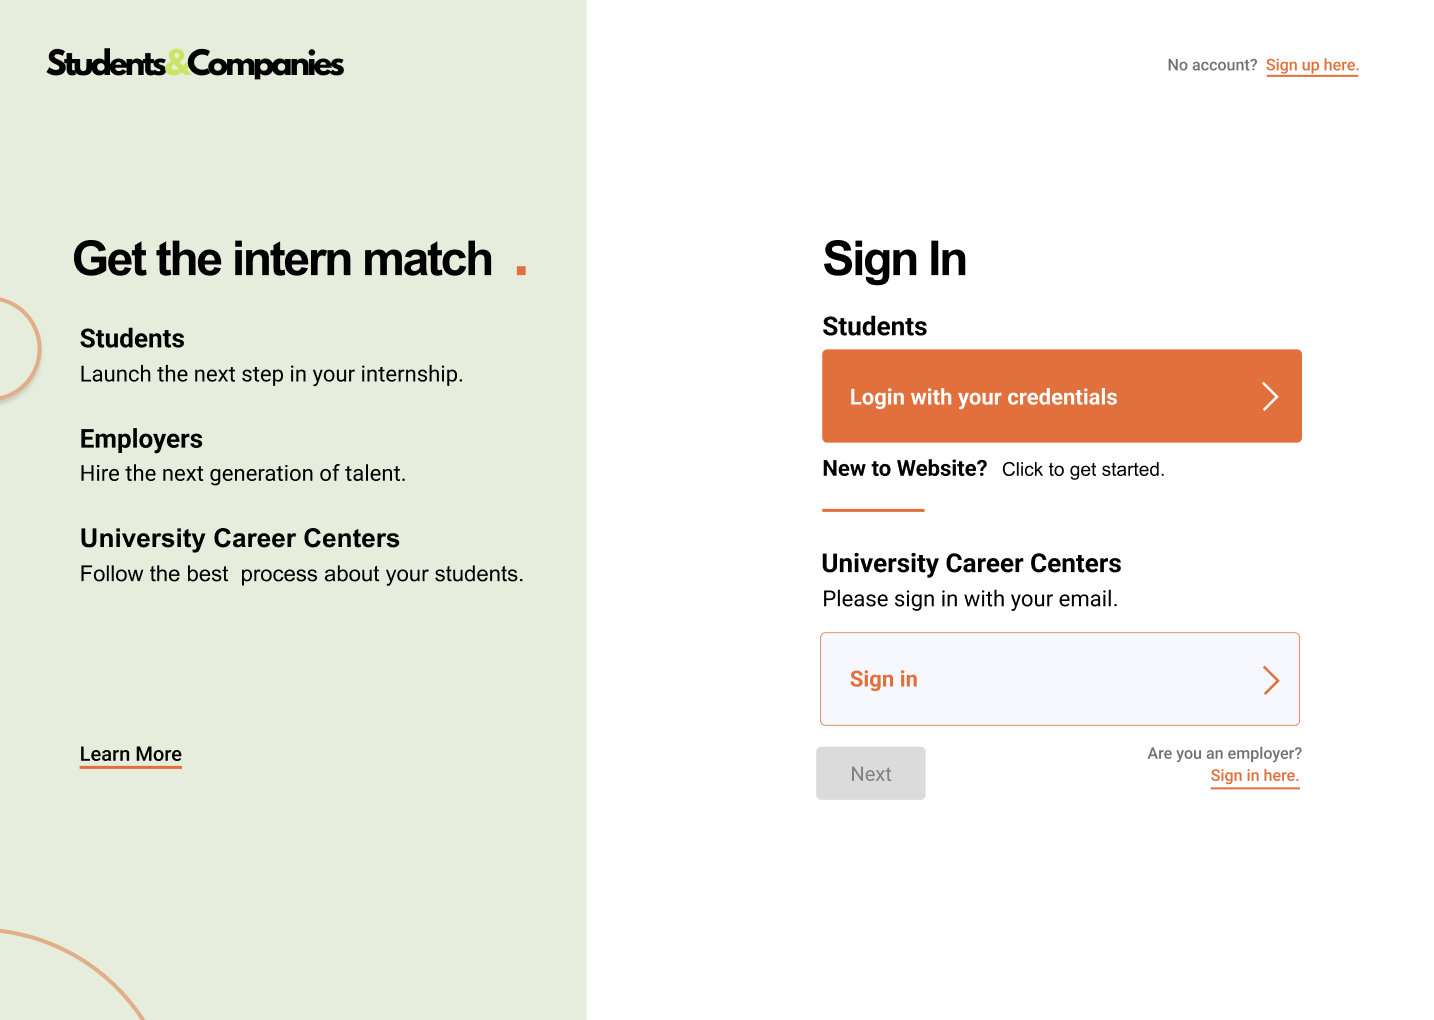
\includegraphics[scale = 0.42]{figures/UserInterfaces/General/HomeSignIn.png}
    \caption{Home Sign In Page}
     \centering
\end{figure}

\begin{figure}[H]
    \centering
    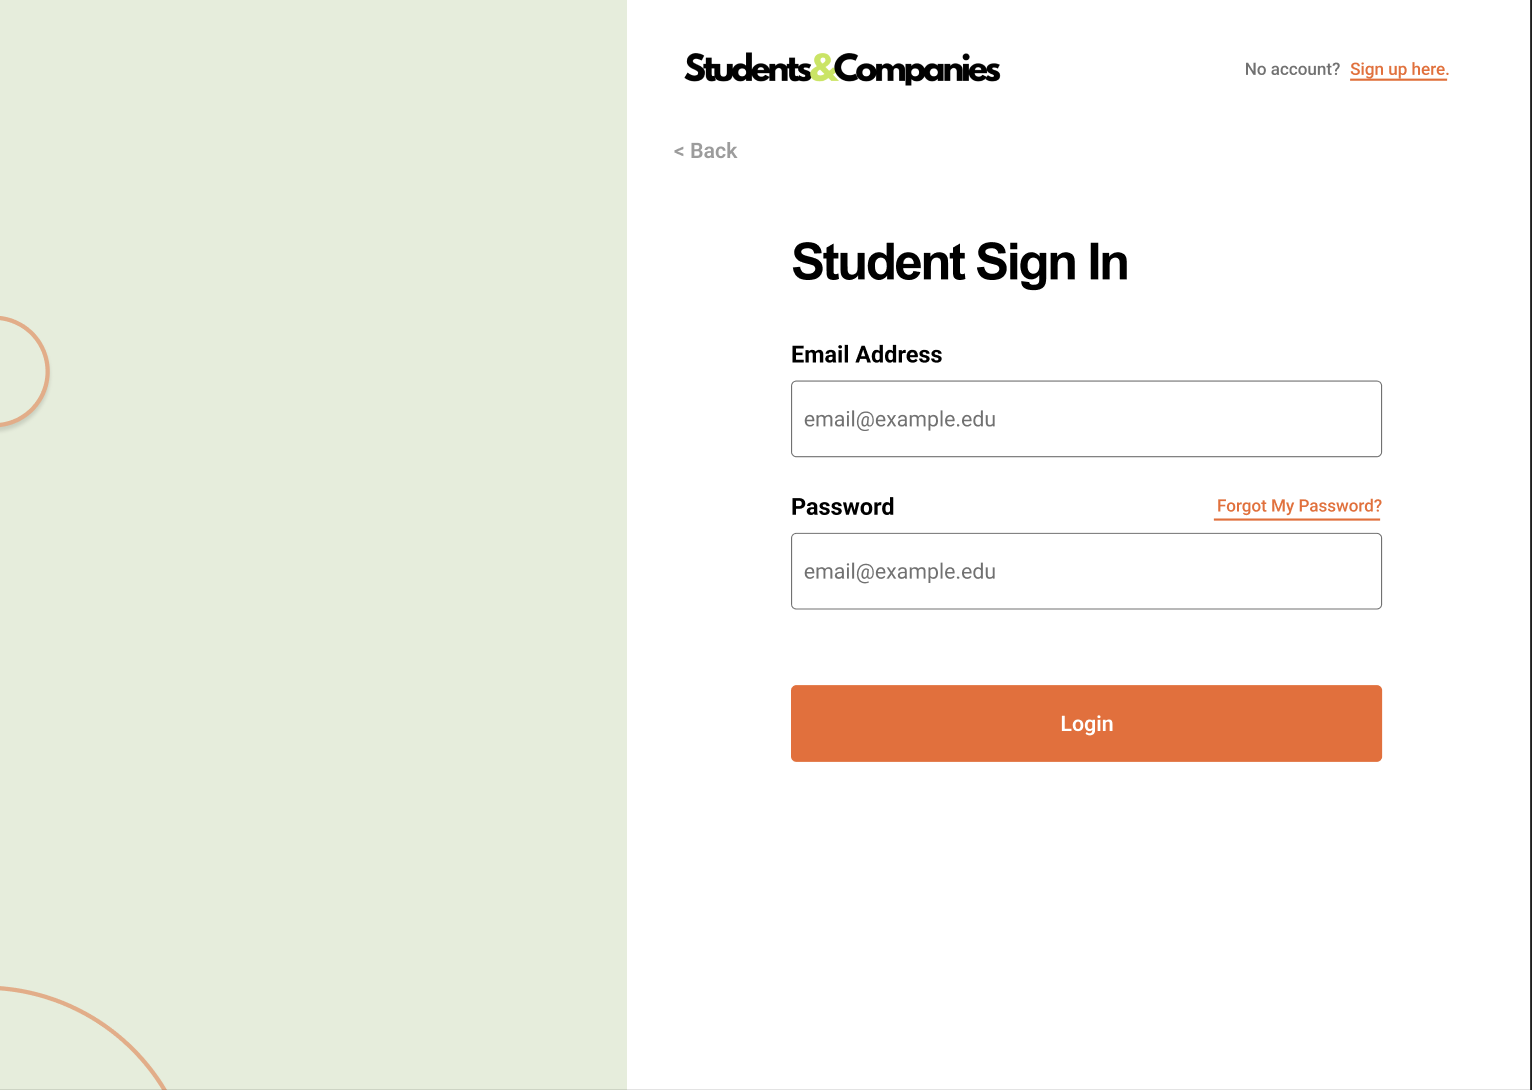
\includegraphics[scale = 0.40]{figures/UserInterfaces/General/StudentSignIn.png}
    \caption{Student Sign In}
     \centering
\end{figure}
\begin{figure}[H]
    \centering
\begin{figure}[H]
    \centering
    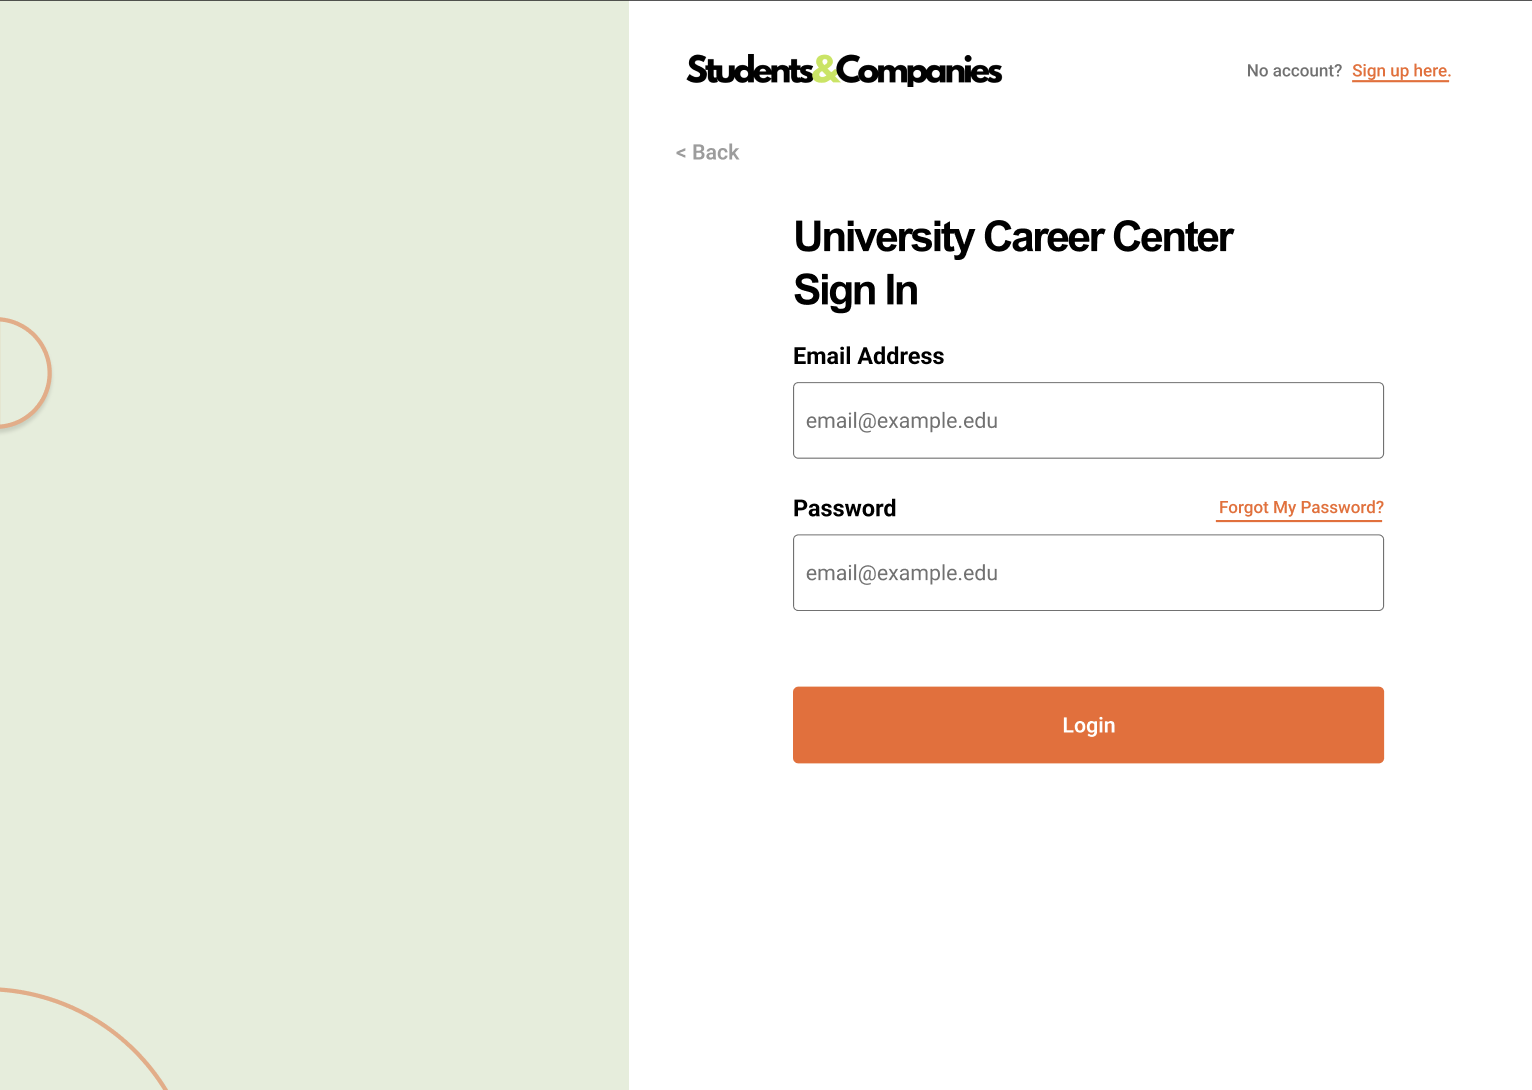
\includegraphics[scale = 0.40]{figures/UserInterfaces/General/UniversitySignIn.png}
    \caption{University Sign In}
     \centering
\end{figure}
    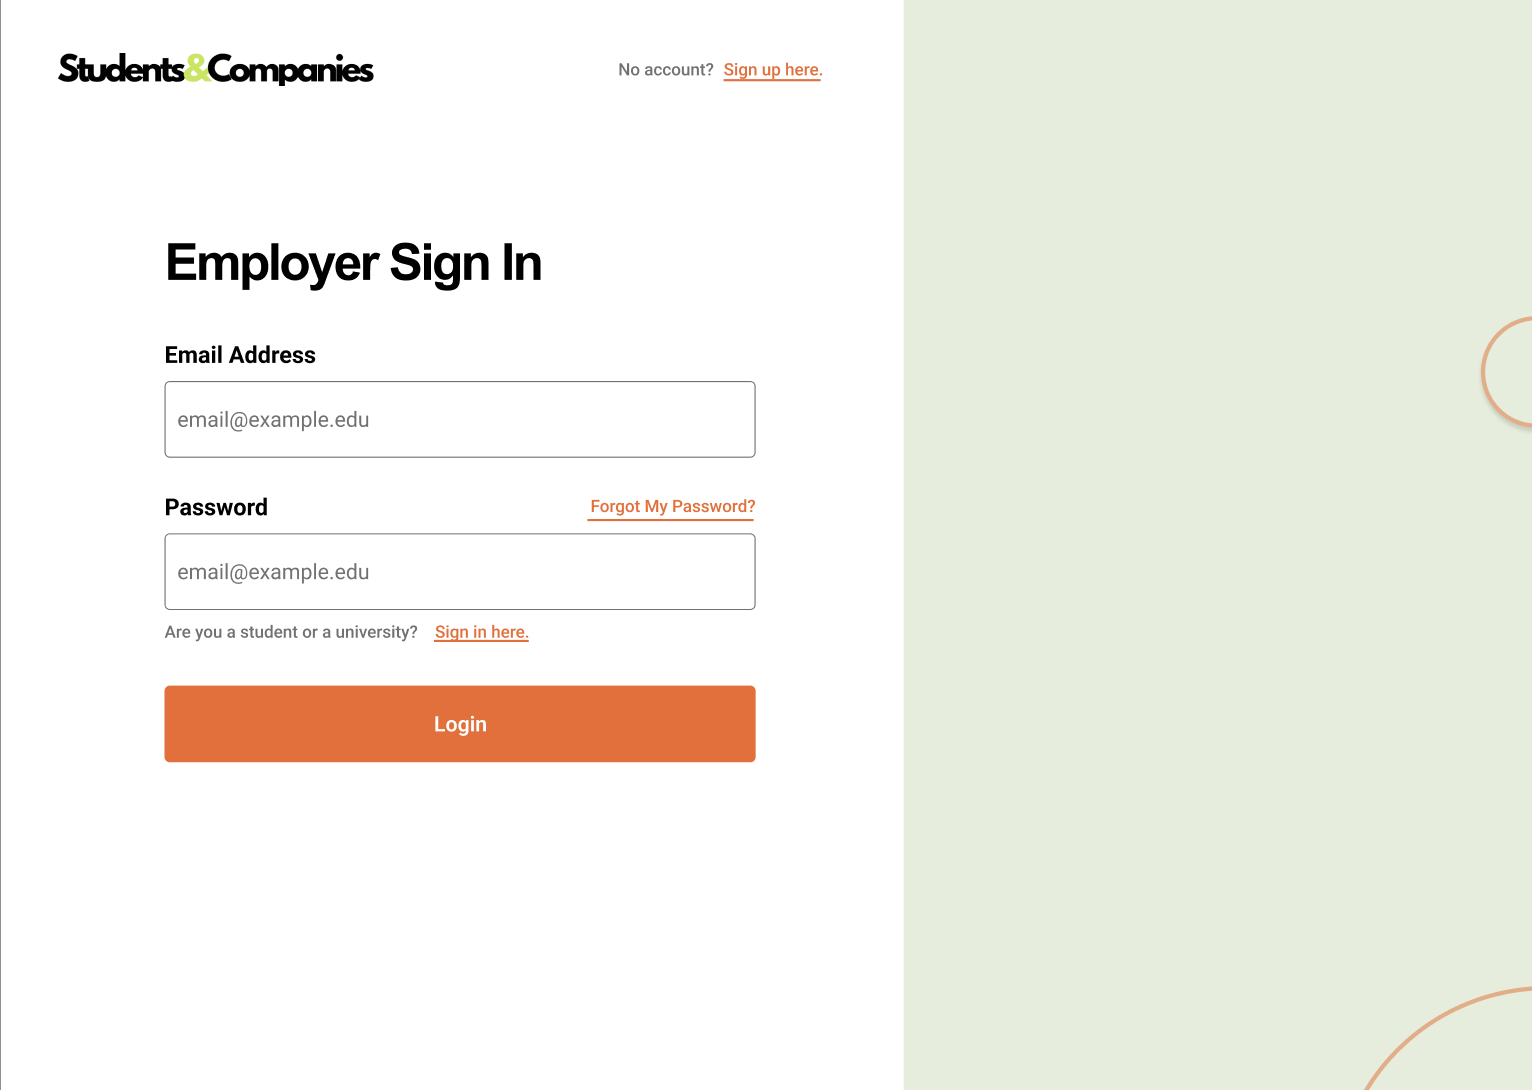
\includegraphics[scale = 0.40]{figures/UserInterfaces/General/EmployerSignIn.png}
    \caption{Employer Sign In}
     \centering
\end{figure}

\newpage
\subsubsection*{Student Pages}
This section represents the pages that will be displayed to the student users, who have already registered in the system and provided the necessary credentials. The system offers a variety of functionalities, such as the ability for students to apply for internship postings, update their profiles, and receive recommendations and suggestions generated by the system. These functionalities and more are detailed in the design presented in this section.

\begin{figure}[H]
    \centering
    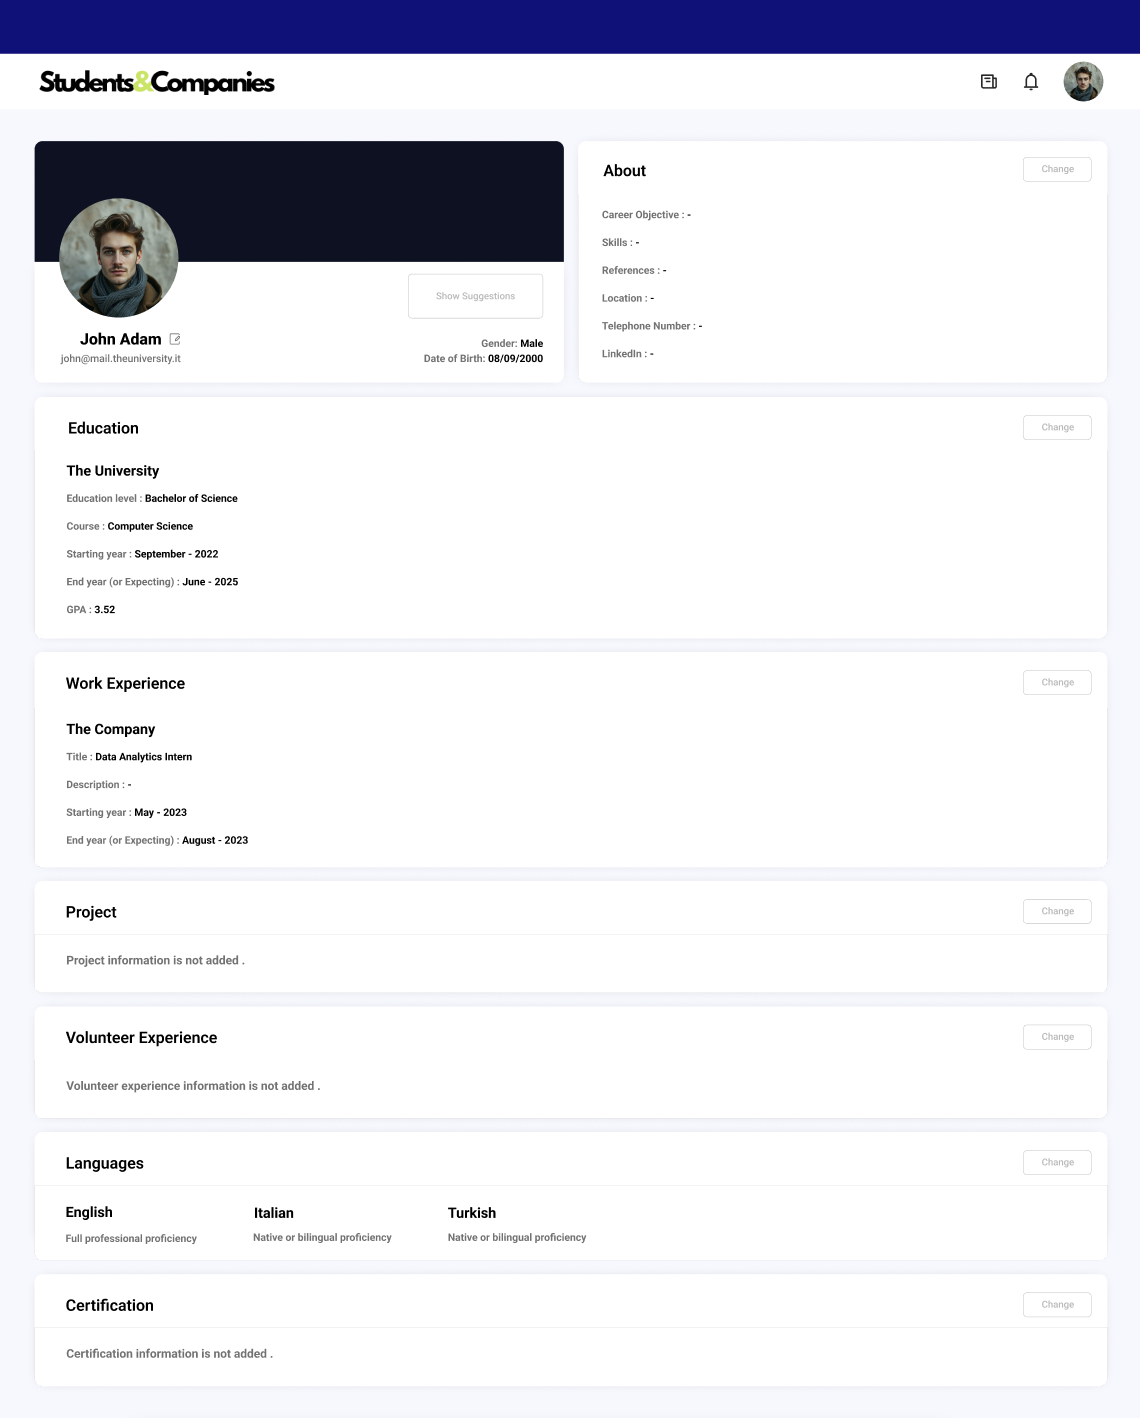
\includegraphics[scale = 0.35
    ]{figures/UserInterfaces/Student/Profile.png}
    \caption{Student Profile Details}
     \centering
\end{figure}
\begin{figure}[H]
    \centering
    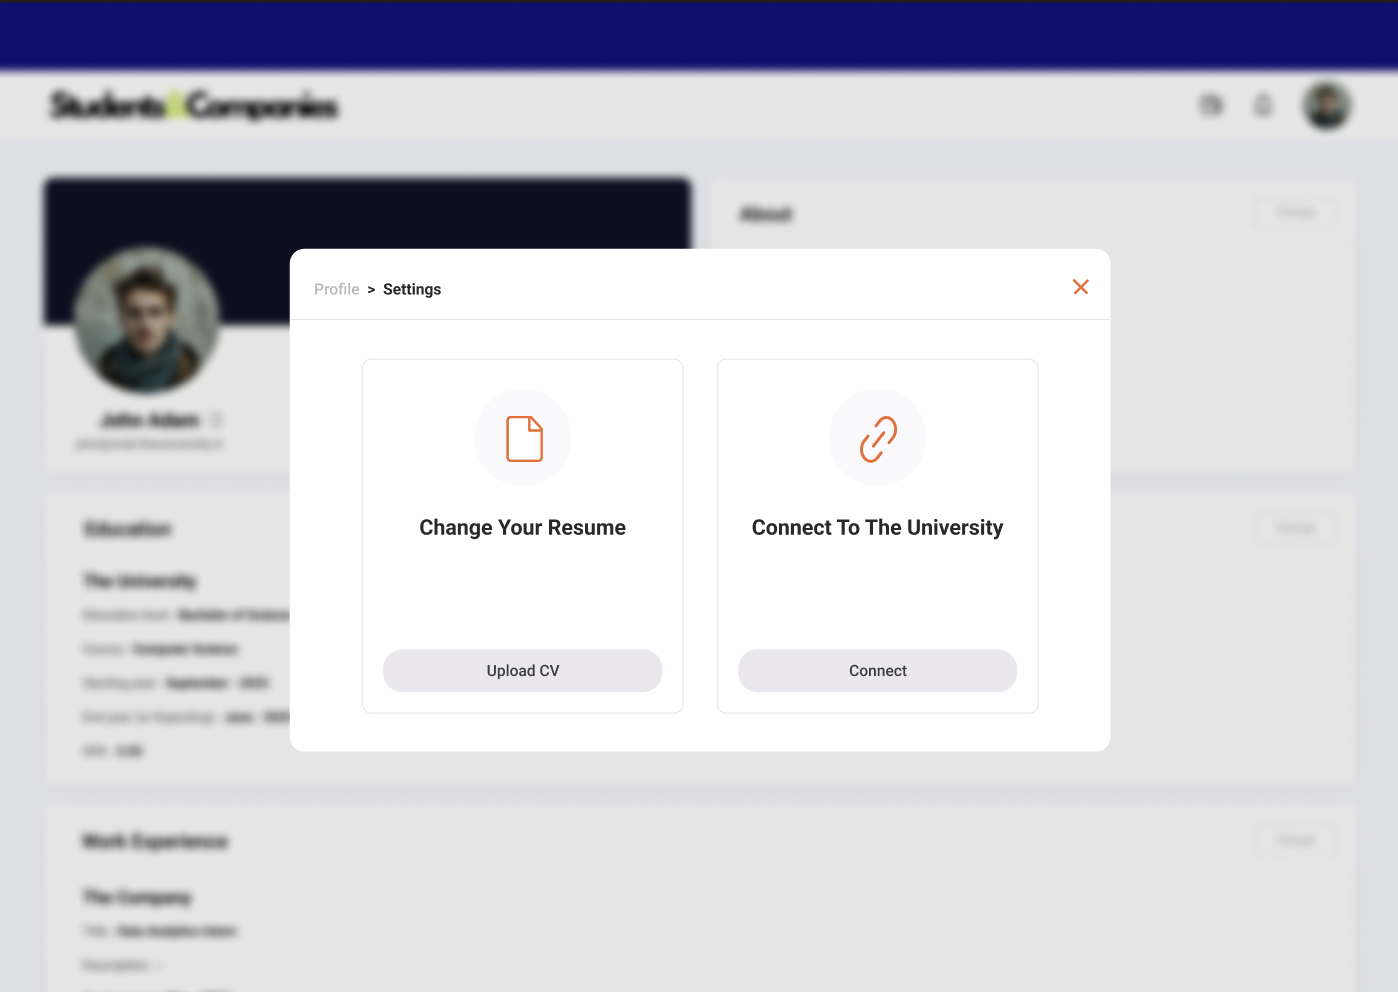
\includegraphics[scale = 0.42]{figures/UserInterfaces/Student/Settings.png}
    \caption{Student Settings}
     \centering
\end{figure}
\begin{figure}[H]
    \centering
    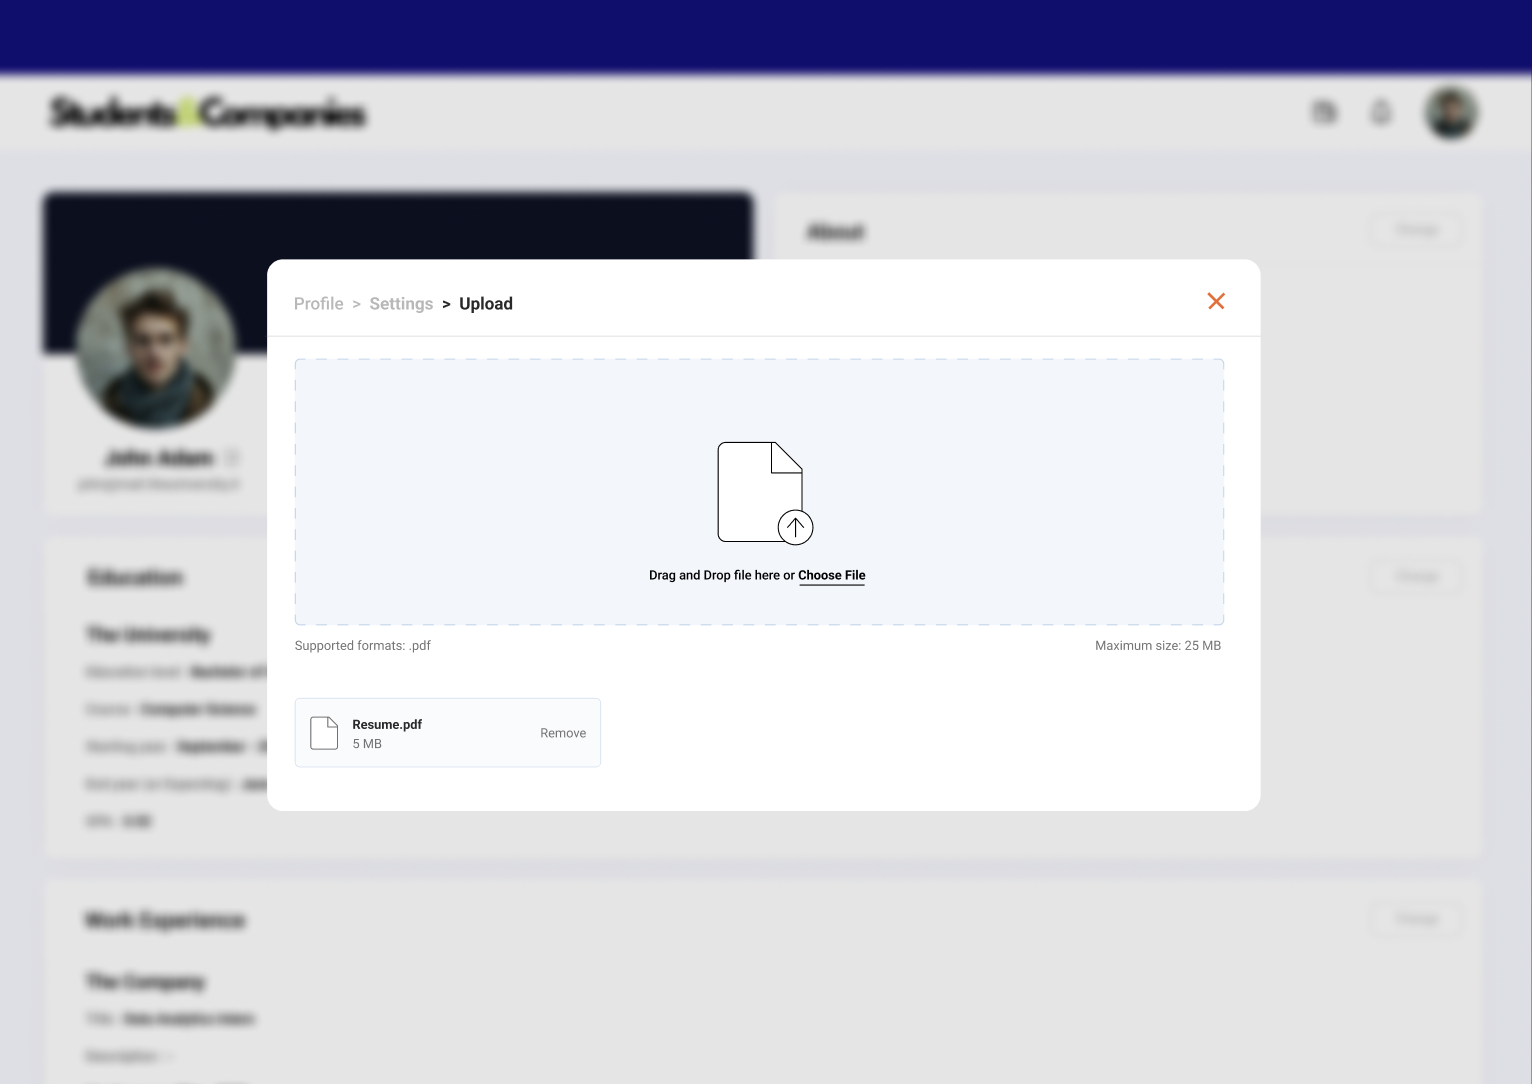
\includegraphics[scale = 0.42]{figures/UserInterfaces/Student/UploadCv.png}
    \caption{Student Update CV}
     \centering
\end{figure}

    \begin{figure}[H]
    \centering
    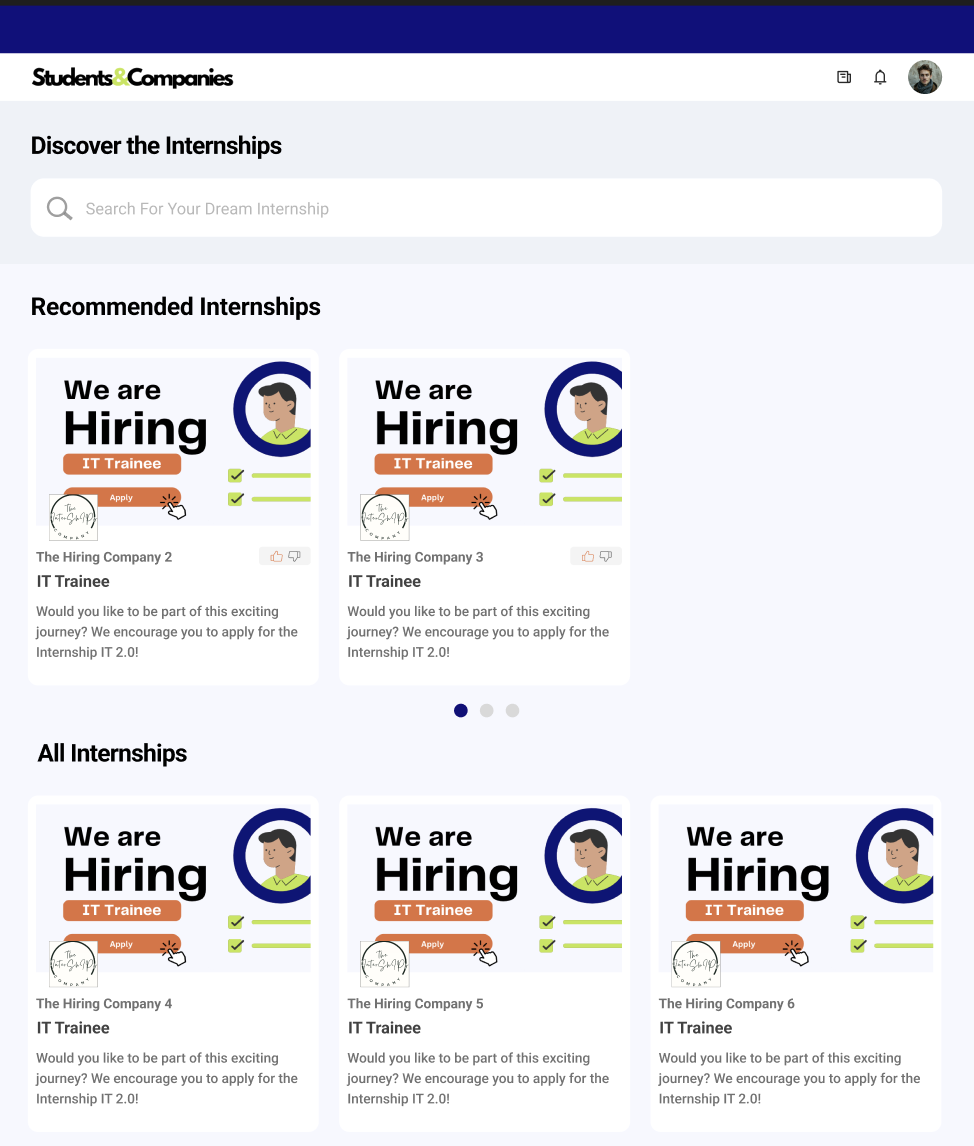
\includegraphics[scale = 0.40]{figures/UserInterfaces/Student/HomePage1.png}
    \caption{Student Home Page 1}
     \centering
\end{figure}

\begin{figure}[H]
    \centering
    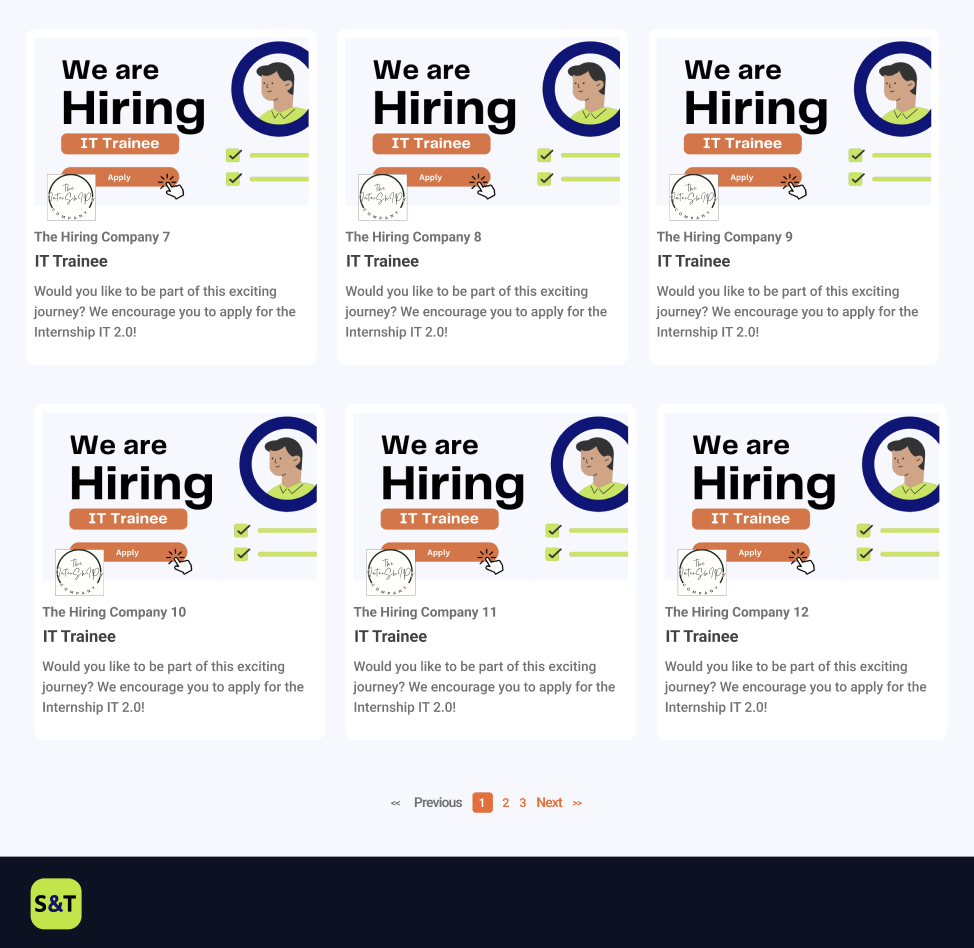
\includegraphics[scale = 0.40]{figures/UserInterfaces/Student/HomePage2.png}
    \caption{Student Home Page 2}
     \centering
\end{figure}

\begin{figure}[H]
    \centering
    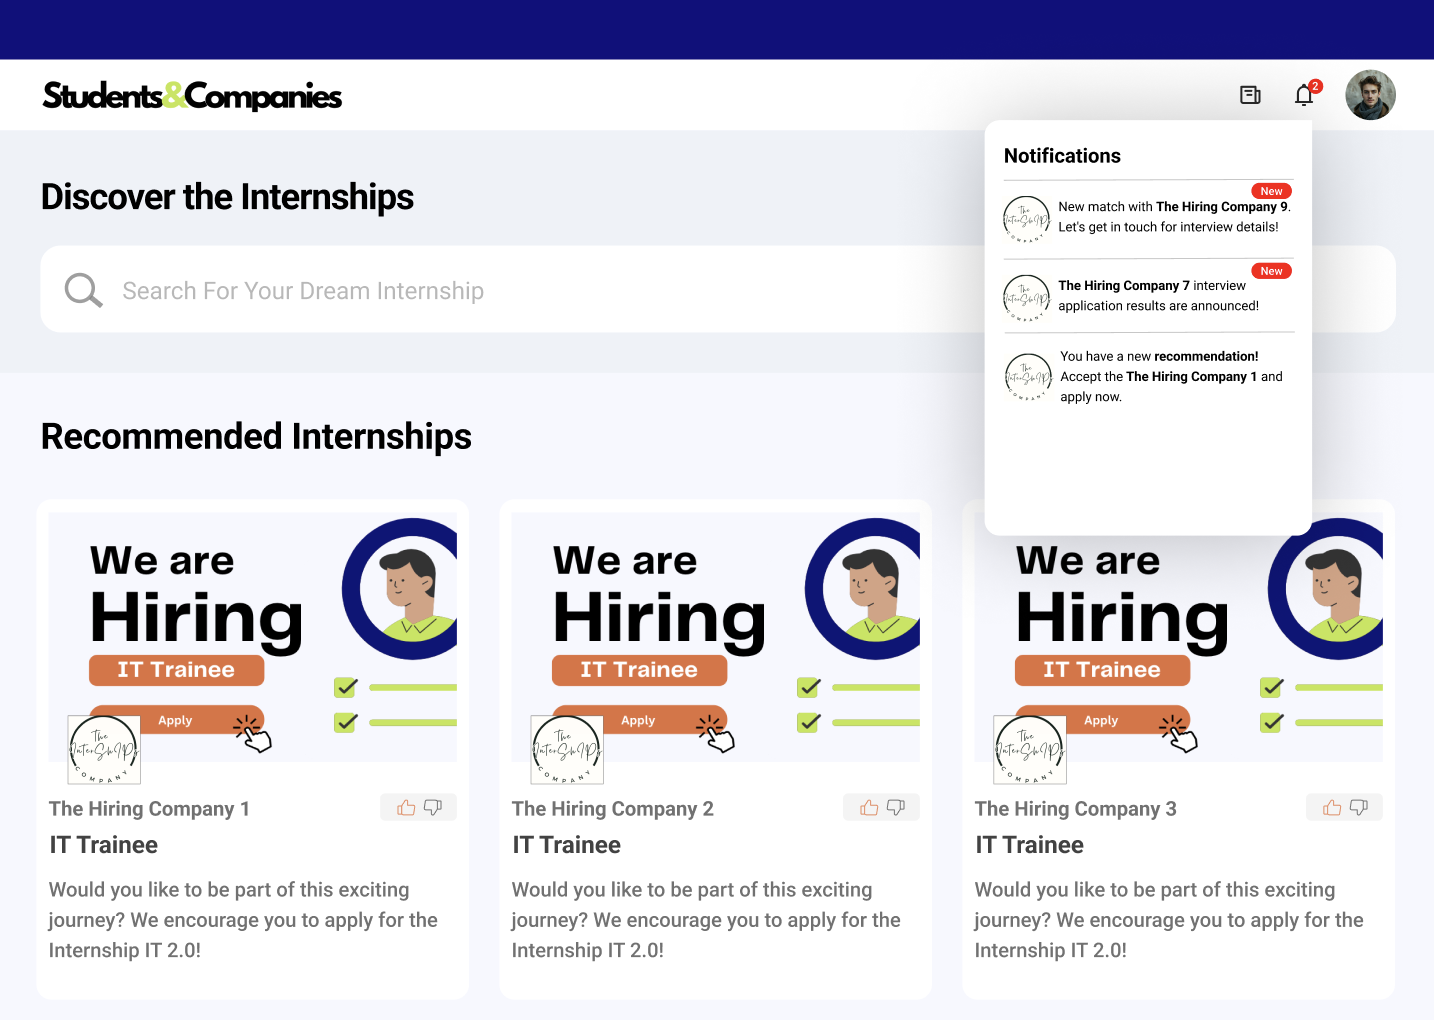
\includegraphics[scale = 0.435]{figures/UserInterfaces/Student/Notifications.png}
    \caption{Student Notifications}
     \centering
\end{figure}

\begin{figure}[H]
    \centering
    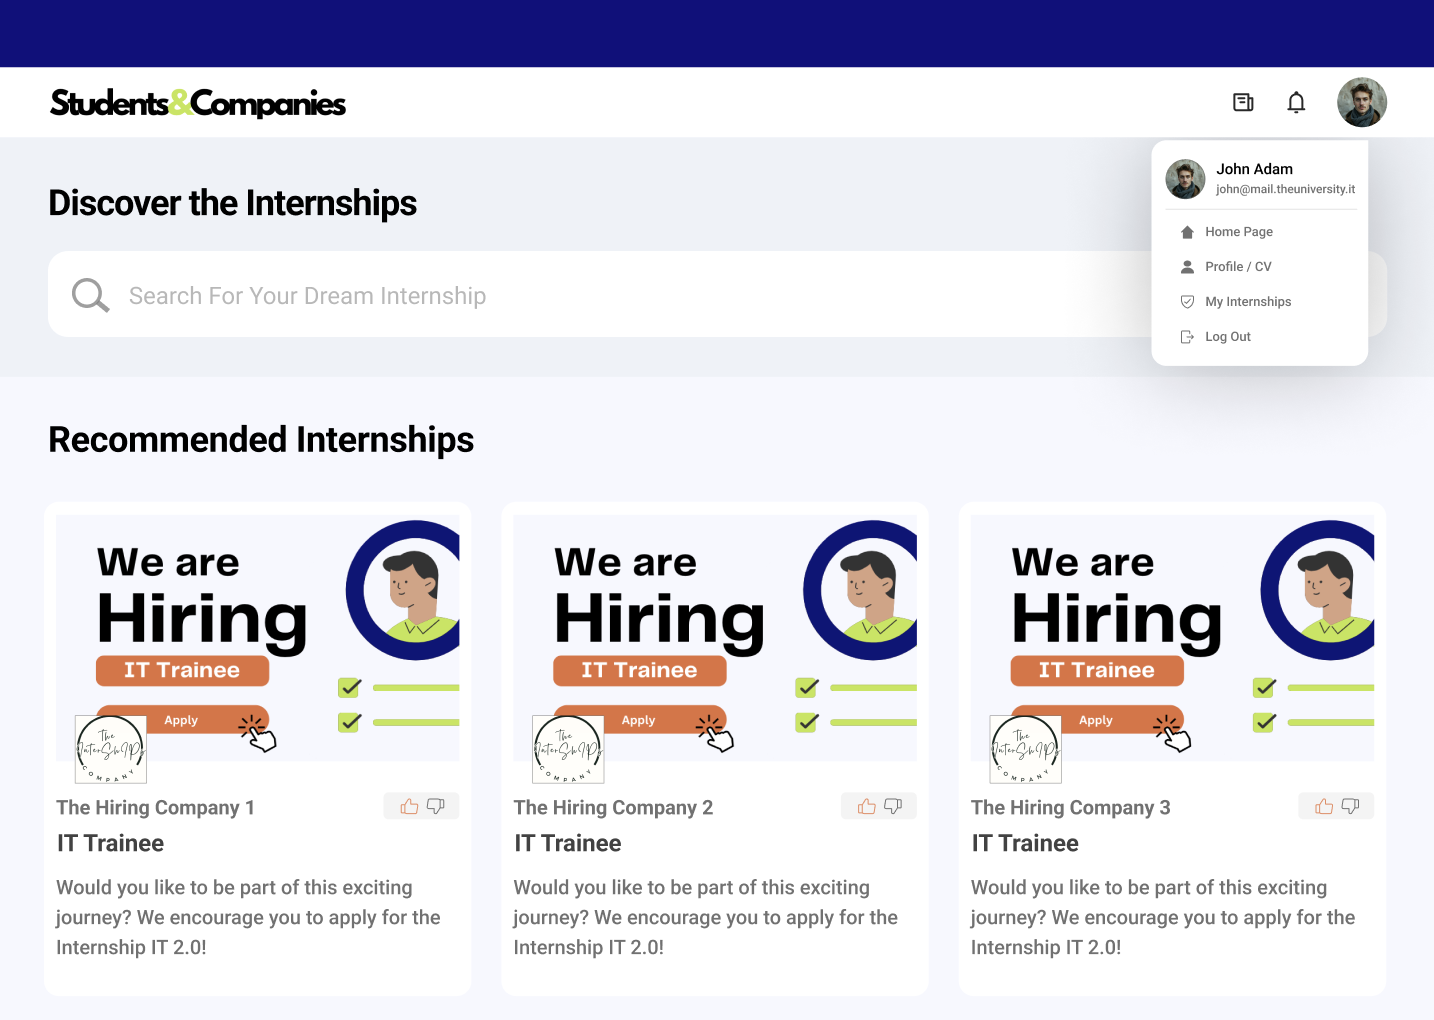
\includegraphics[scale = 0.40]{figures/UserInterfaces/Student/ProfileMenu.png}
    \caption{Student Profile Menu}
     \centering
\end{figure}

\begin{figure}[H]
    \centering
    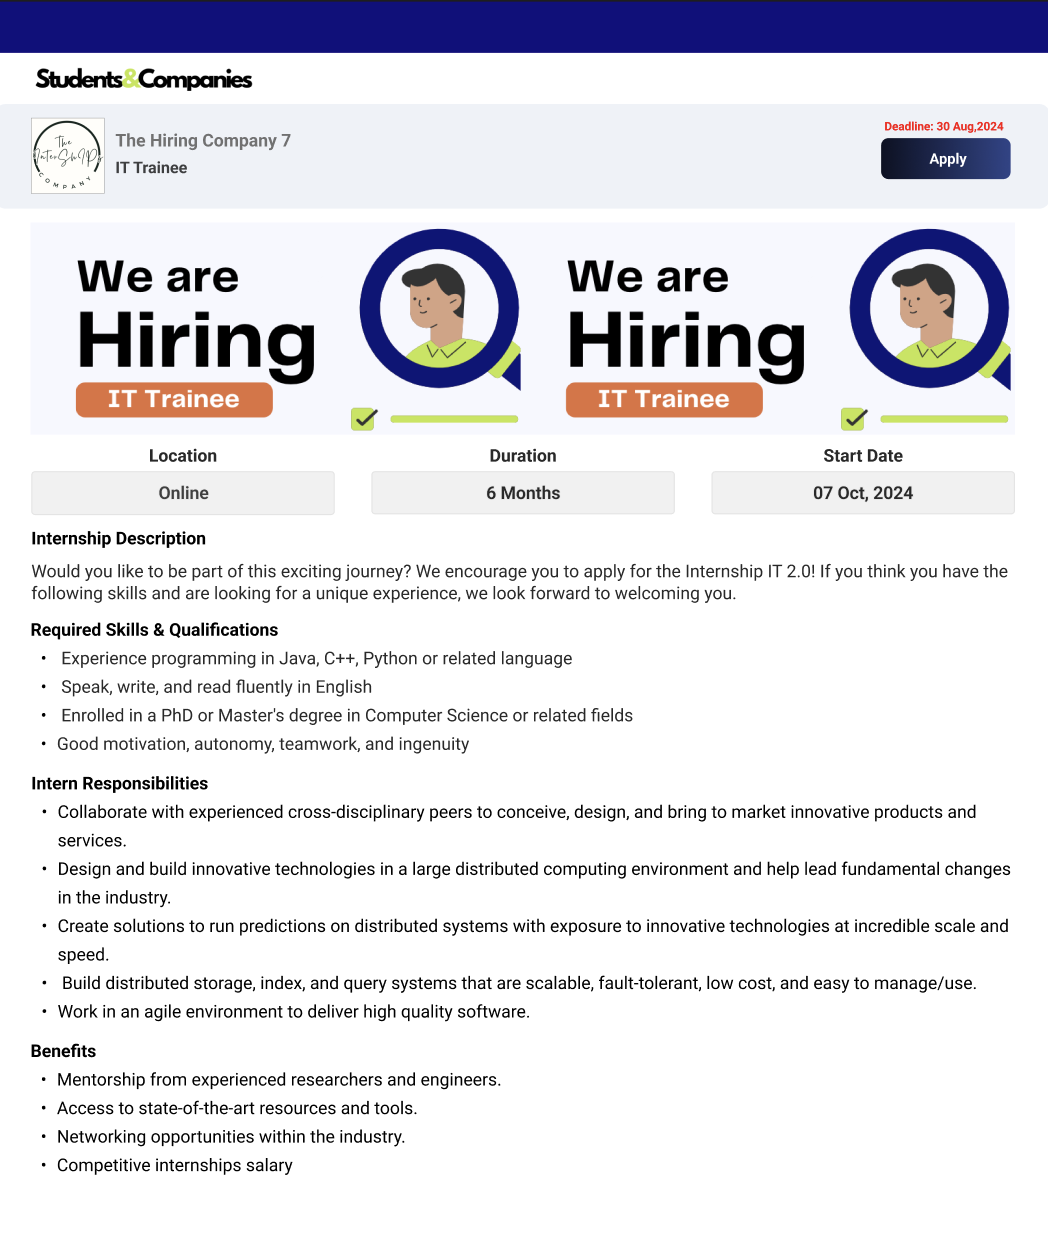
\includegraphics[scale = 0.55]{figures/UserInterfaces/Student/AdvertisementPage.png}
    \caption{Advertisement Details Page}
     \centering
\end{figure}

\begin{figure}[H]
    \centering
    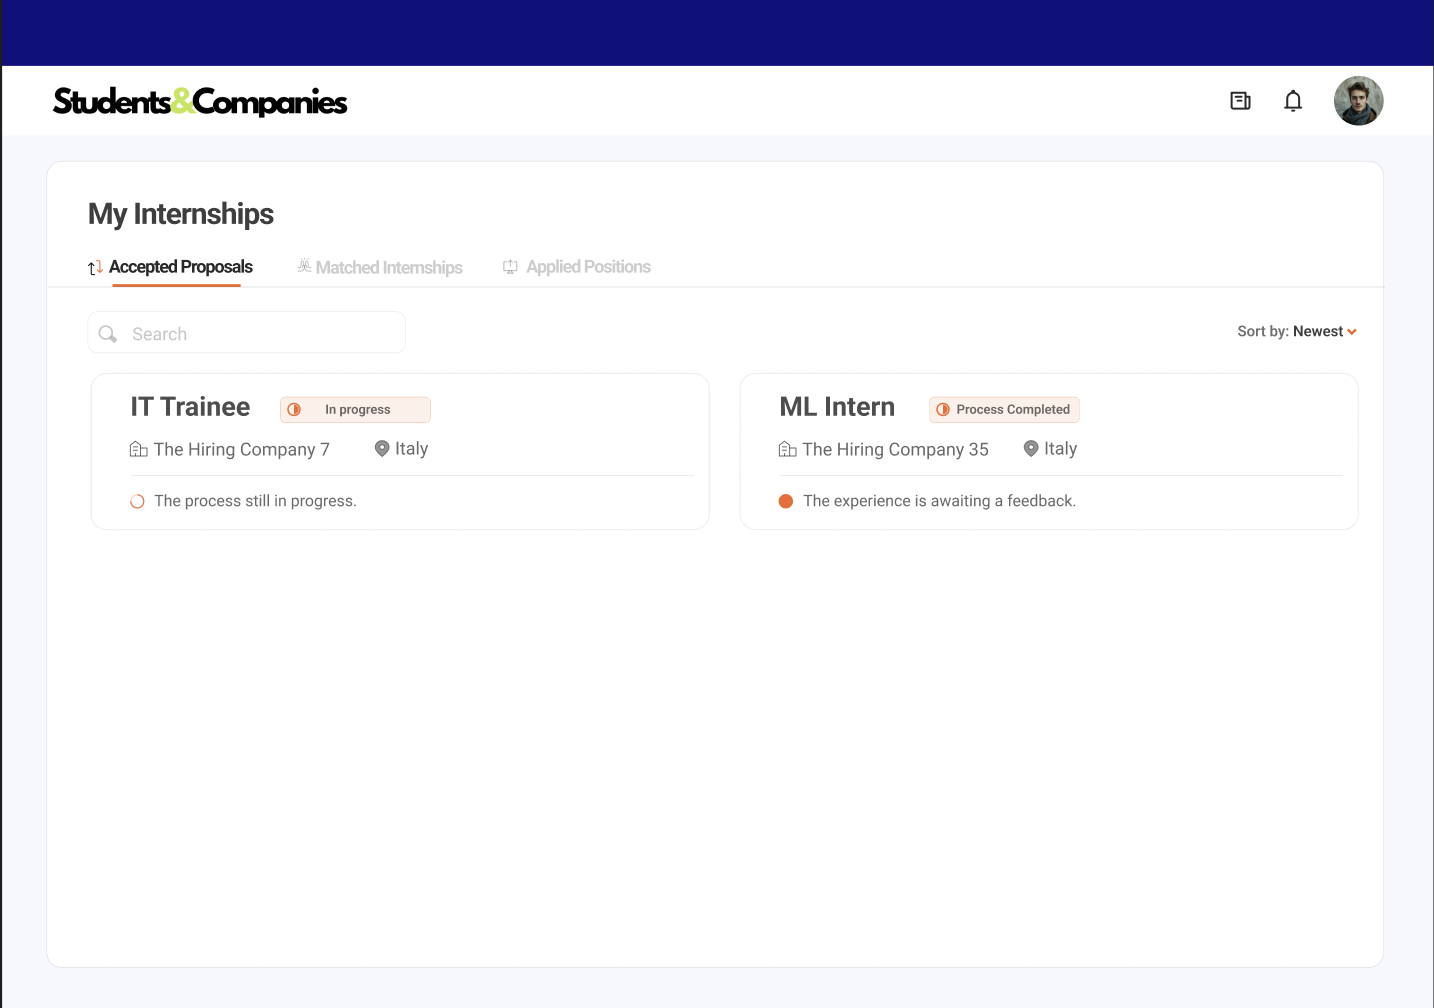
\includegraphics[scale = 0.42]{figures/UserInterfaces/Student/AcceptedProposals.png}
    \caption{Student Accepted Internships}
     \centering
\end{figure}
\begin{figure}[H]
    \centering
    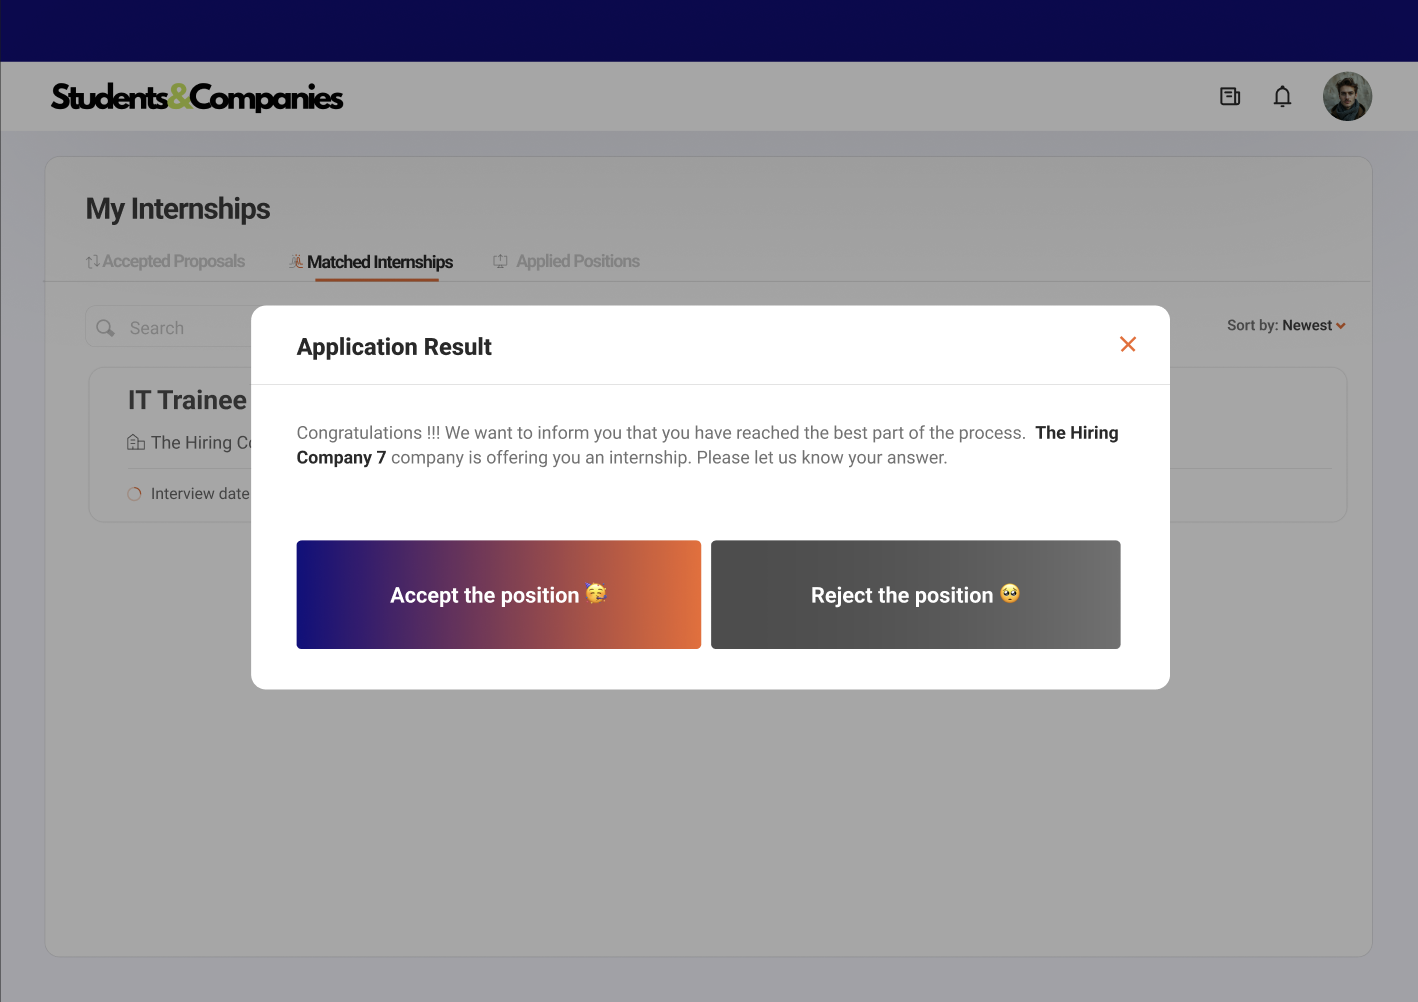
\includegraphics[scale = 0.42]{figures/UserInterfaces/Student/AcceptPop-up.png}
    \caption{Accepting the position}
     \centering
\end{figure}


\begin{figure}[H]
    \centering
    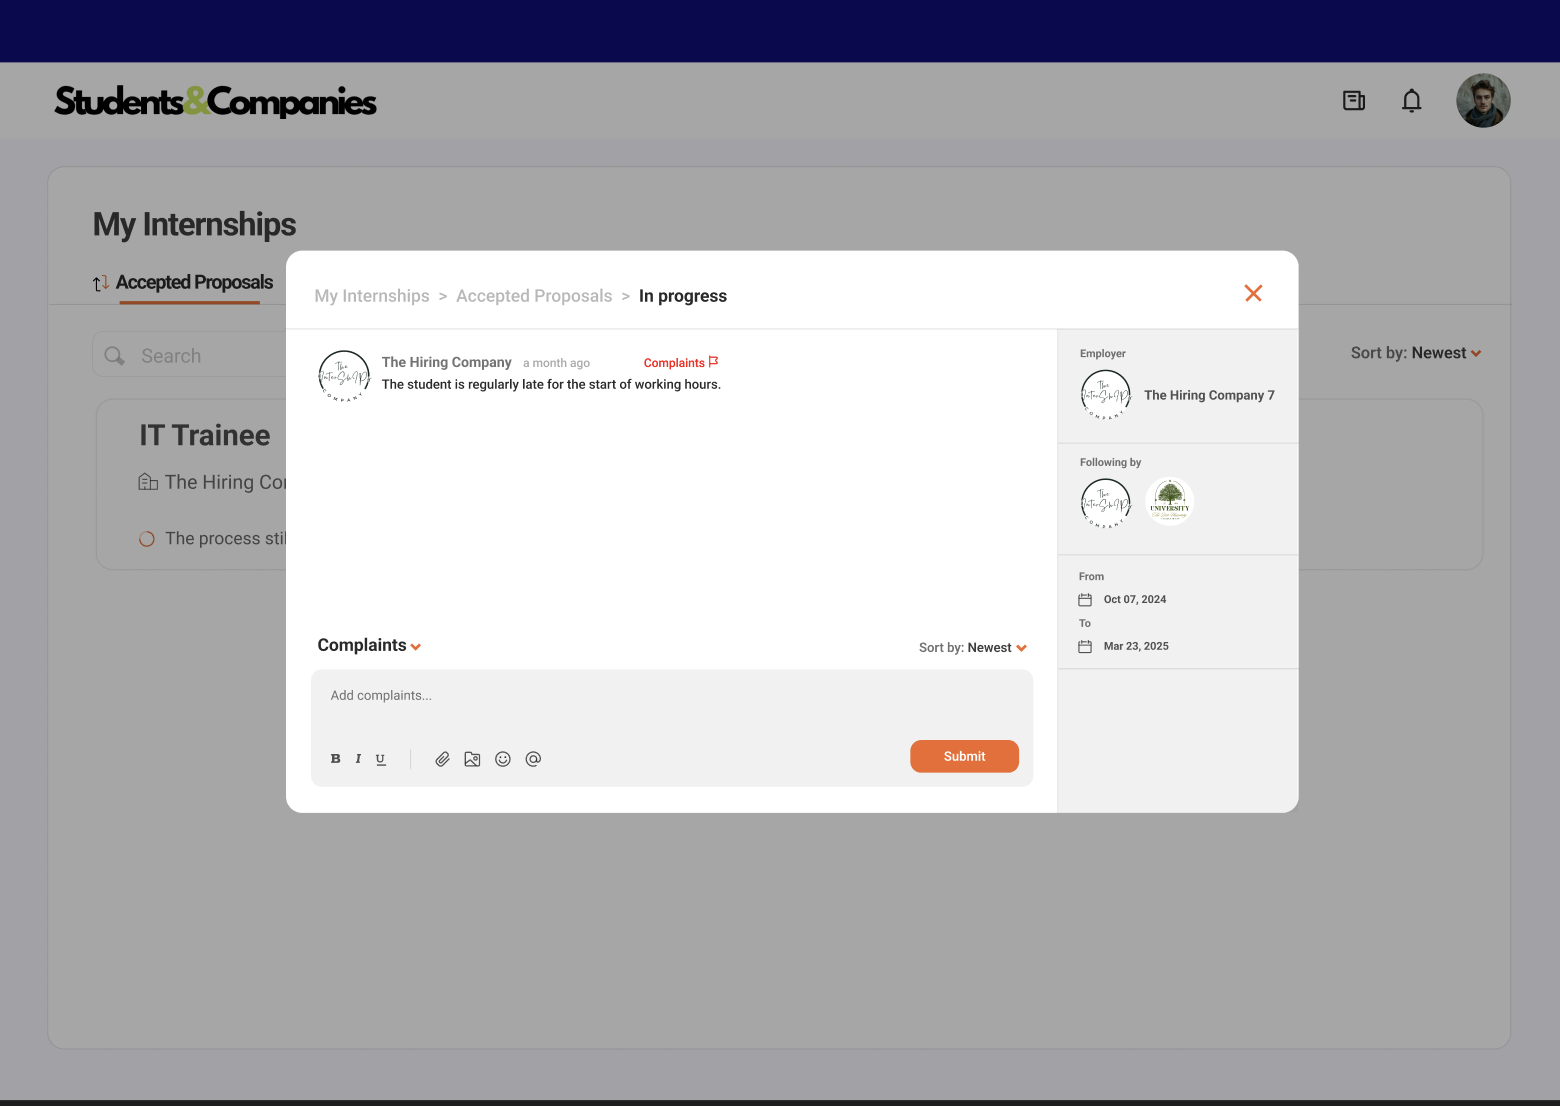
\includegraphics[scale = 0.42]{figures/UserInterfaces/Student/StudentComplaints.png}
    \caption{Student Ongoing Internship Complaints}
     \centering
\end{figure}
\begin{figure}[H]
    \centering
    \includegraphics[scale = 0.42]{figures/UserInterfaces/Student/MatchedInternships.png}
    \caption{Student Matched Internships}
     \centering
\end{figure}

\begin{figure}[H]
    \centering
    \includegraphics[scale = 0.42]{figures/UserInterfaces/Student/BookingPop-up.png}
    \caption{Student Interview Schedule}
     \centering
\end{figure}

\begin{figure}[H]
    \centering
    \includegraphics[scale = 0.42]{figures/UserInterfaces/Student/Feedback.png}
    \caption{Student Feedback}
     \centering
\end{figure}

\begin{figure}[H]
    \centering
    \includegraphics[scale = 0.42]{figures/UserInterfaces/Student/AppliedPositions.png}
    \caption{Student Applied Internships}
     \centering
\end{figure}
\begin{figure}[H]
    \centering
    \includegraphics[scale = 0.42]{figures/UserInterfaces/Student/SuggestionNotification.png}
    \caption{Student Suggestions Notification}
     \centering
\end{figure}
\begin{figure}[H]
    \centering
    \includegraphics[scale = 0.65]{figures/UserInterfaces/Student/CVSuggestion.png}
    \caption{Student CV Suggestion Template}
     \centering
\end{figure}
\newpage
\subsubsection*{Company Pages}
This section contains the pages design that will be displayed to company users after they provide the necessary credentials. Also, in this section presents the system designs that allow company users to create internship postings according to their needs, accept students recommended by the system or those who apply normally, and perform various functionalities such as interview scheduling, offering and more internship positions to students.
\begin{figure}[H]
    \centering
    \includegraphics[scale = 0.42]{figures/UserInterfaces/Company/CompanyHome.png}
    \caption{Company Home Page}
     \centering
\end{figure}
\begin{figure}[H]
    \centering
    \includegraphics[scale = 0.40]{figures/UserInterfaces/Company/CompanySuggestion.png}
    \caption{Company Advertisement Suggestion Template}
     \centering
\end{figure}
\begin{figure}[H]
    \centering
    \includegraphics[scale = 0.42]{figures/UserInterfaces/Company/CreateInternship1.png}
    \caption{Create Internship Page 1}
     \centering
\end{figure}
\begin{figure}[H]
    \centering
    \includegraphics[scale = 0.40]{figures/UserInterfaces/Company/CreateInternship2.png}
    \caption{Create Internship Page 2}
     \centering
\end{figure}
\begin{figure}[H]
    \centering
    \includegraphics[scale = 0.40]{figures/UserInterfaces/Company/CreateInternship3.png}
    \caption{Create Internship Page 3}
     \centering
\end{figure}
\begin{figure}[H]
    \centering
    \includegraphics[scale = 0.40]{figures/UserInterfaces/Company/ManageInternships.png}
    \caption{Manage Internships Page}
     \centering
\end{figure}
\begin{figure}[H]
    \centering
    \includegraphics[scale = 0.42]{figures/UserInterfaces/Company/AllCandidatesCompany.png}
    \caption{All Candidates Page}
     \centering
\end{figure}
\begin{figure}[H]
    \centering
    \includegraphics[scale = 0.42]{figures/UserInterfaces/Company/AcceptedProposalCompany.png}
    \caption{Company Accepted Proposals Page}
     \centering
\end{figure}
\begin{figure}[H]
    \centering
    \includegraphics[scale = 0.42]{figures/UserInterfaces/Company/CompanyComplaints.png}
    \caption{Company Ongoing Internship Complaints Page}
     \centering
\end{figure}
\begin{figure}[H]
    \centering
    \includegraphics[scale = 0.42]{figures/UserInterfaces/Company/FeedbackCompany.png}
    \caption{Feedback}
     \centering
\end{figure}
\begin{figure}[H]
    \centering
    \includegraphics[scale = 0.42]{figures/UserInterfaces/Company/MatchedCompany.png}
    \caption{Company Matched Internships Page}
     \centering
\end{figure}
\begin{figure}[H]
    \centering
    \includegraphics[scale = 0.42]{figures/UserInterfaces/Company/Scheduling.png}
    \caption{Company Interview Scheduling}
     \centering
\end{figure}
\begin{figure}[H]
    \centering
    \includegraphics[scale = 0.42]{figures/UserInterfaces/Company/InterviewLink.png}
    \caption{Interview Link}
     \centering
\end{figure}
\begin{figure}[H]
    \centering
    \includegraphics[scale = 0.42]{figures/UserInterfaces/Company/SelectionProcess.png}
    \caption{Student Selection Process Pop-Up}
     \centering
\end{figure}
\begin{figure}[H]
    \centering
    \includegraphics[scale = 0.42]{figures/UserInterfaces/Company/ApprovedProfiles.png}
    \caption{Company Approved Profiles Page}
     \centering
\end{figure}
\begin{figure}[H]
    \centering
    \includegraphics[scale = 0.42]{figures/UserInterfaces/Company/NotificationsCompany.png}
    \caption{Company Notifications}
     \centering
\end{figure}
\newpage
\subsubsection*{University Pages}
This section includes the page designs that university representatives can access after entering the necessary credentials into the system. The system provides interface that enable university representatives to monitor their students' internship processes, view any complaints that may arise during the internship, and, when necessary, interrupt the internship process.
\begin{figure}[H]
    \centering
    \includegraphics[scale = 0.40]{figures/UserInterfaces/University/UniversityHomePage.png}
    \caption{University Home Page}
     \centering
\end{figure}
\begin{figure}[H]
    \centering
    \includegraphics[scale = 0.40]{figures/UserInterfaces/University/InterruptPage.png}
    \caption{University Interrupt Page}
     \centering
\end{figure}
\begin{figure}[H]
    \centering
    \includegraphics[scale = 0.40]{figures/UserInterfaces/University/University Notifications.png}
    \caption{University Notifications}
     \centering
\end{figure}
\newpage
\section{Requirements Traceability}

\begin{center}
    \begin{tabular}{|C{3cm}|p{10cm}|}
    \hline
    \multicolumn{2}{|c|}{\parbox{13cm}{R1: The system must allow a student who wants to register to sign up.}} \\
    \hline
    \centering C0 & DB Manager \\ 
    \hline
    \centering C3 & Authentication Manager \\ 
    \hline
    \centering C6 & Recommendation Manager \\ 
    \hline
    \centering C8 & Notification Manager \\ 
    \hline
    \centering C9 & Model \\ 
    \hline
    \centering C10 & Email Service Provider \\ 
    \hline
    \centering C11 & Notification Provider \\ 
    \hline
    \centering C13 & University Login Service \\ 
    \hline
    \end{tabular}
\end{center}

\begin{center}
    \begin{tabular}{|C{3cm}|p{10cm}|}
    \hline
    \multicolumn{2}{|c|}{\parbox{13cm}{R2: The system must allow a company who wants to register to sign up.}} \\
    \hline
    \centering C0 & DB Manager \\ 
    \hline
    \centering C3 & Authentication Manager \\ 
    \hline
    \centering C6 & Recommendation Manager \\ 
    \hline
    \centering C9 & Model \\ 
    \hline
    \centering C10 & Email Service Provider \\ 
    \hline
    \end{tabular}
\end{center}

\begin{center}
    \begin{tabular}{|C{3cm}|p{10cm}|}
    \hline
    \multicolumn{2}{|c|}{\parbox{13cm}{R3: The system must allow a university who wants to register to sign up.}} \\
    \hline
    \centering C0 & DB Manager \\ 
    \hline
    \centering C3 & Authentication Manager \\ 
    \hline
    \centering C8 & Notification Manager \\ 
    \hline
    \centering C9 & Model \\ 
    \hline
    \centering C10 & Email Service Provider \\ 
    \hline
    \centering C12 & National Education Dictionary API\\
    \hline
    \end{tabular}
\end{center}

\begin{center}
    \begin{tabular}{|C{3cm}|p{10cm}|}
    \hline
    \multicolumn{2}{|c|}{\parbox{13cm}{R4: The system must allow registered users to sign in using their credentials.}} \\
    \hline
    \centering C0 & DB Manager \\ 
    \hline
    \centering C1 & Dashboard Manager \\ 
    \hline
    \centering C2 & Account Manager \\ 
    \hline
    \centering C3 & Authentication Manager \\ 
    \hline
    \centering C9 & Model \\ 
    \hline
    \end{tabular}
\end{center}

\begin{center}
    \begin{tabular}{|C{3cm}|p{10cm}|}
    \hline
    \multicolumn{2}{|c|}{\parbox{13cm}{R6: The system must be able to send notifications to all users.}} \\
    \hline
    \centering C1 & Dashboard Manager \\ 
    \hline
    \centering C4 & Internship Manager \\ 
    \hline
    \centering C5 & Comment Manager \\ 
    \hline
    \centering C6 & Recommendation Manager \\ 
    \hline
    \centering C7 & Interaction Manager \\ 
    \hline
    \centering C8 & Notification Manager \\ 
    \hline
    \centering C10 & Email Service Provider \\ 
    \hline
    \centering C11 & Notification Provider \\ 
    \hline
    
    \end{tabular}
\end{center}

\begin{center}
    \begin{tabular}{|C{3cm}|p{10cm}|}
    \hline
    \multicolumn{2}{|c|}{\parbox{13cm}{R7: The system must allow registered students to upload their CVs on the platform.}} \\
    \hline
    \centering C0 & DB Manager \\ 
    \hline
    \centering C1 & Dashboard Manager \\ 
    \hline
    \centering C2 & Account Manager \\ 
    \hline
    \centering C6 & Recommendation Manager \\ 
    \hline
    \centering C8 & Notification Manager \\ 
    \hline
    \centering C9 & Model \\ 
    \hline
    \centering C11 & Notification Provider \\ 
    \hline
    \end{tabular}
\end{center}

\begin{center}
    \begin{tabular}{|C{3cm}|p{10cm}|}
    \hline
    \multicolumn{2}{|c|}{\parbox{13cm}{R8: The system must allow registered companies to post internship advertisements.}} \\
    \hline
    \centering C0 & DB Manager \\ 
    \hline
    \centering C1 & Dashboard Manager \\ 
    \hline
    \centering C4 & Internship Manager \\ 
    \hline
    \centering C6 & Recommendation Manager \\ 
    \hline
    \centering C8 & Notification Manager \\ 
    \hline
    \centering C9 & Model \\ 
    \hline
    \centering C11 & Notification Provider \\ 
    \hline
    \end{tabular}
\end{center}
\begin{center}
    \begin{tabular}{|C{3cm}|p{10cm}|}
    \hline
    \multicolumn{2}{|c|}{\parbox{13cm}{R9: The system must allow companies to review students' CVs and select candidates who meet their internship requirements.}} \\
    \hline
    \centering C0 & DB Manager \\ 
    \hline
    \centering C1 & Dashboard Manager \\ 
    \hline
    \centering C2 & Account Manager \\ 
    \hline
    \centering C9 & Model \\ 
    \hline
    \end{tabular}
\end{center}
\begin{center}
    \begin{tabular}{|C{3cm}|p{10cm}|}
    \hline
    \multicolumn{2}{|c|}{\parbox{13cm}{R10: The system must allow students to review internship advertisements and select them if they wish to apply.}} \\
    \hline
    \centering C0 & DB Manager \\ 
    \hline
    \centering C1 & Dashboard Manager \\ 
    \hline
    \centering C4 & Internship Manager \\ 
    \hline
    \centering C9 & Model \\ 
    \hline
    \end{tabular}
\end{center}
\begin{center}
    \begin{tabular}{|C{3cm}|p{10cm}|}
    \hline
    \multicolumn{2}{|c|}{\parbox{13cm}{R11: The system must allow students to manually search for internship opportunities and save them to their favorites.}} \\
    \hline
    \centering C0 & DB Manager \\ 
    \hline
    \centering C1 & Dashboard Manager \\ 
    \hline
    \centering C4 & Internship Manager \\ 
    \hline
    \centering C9 & Model \\ 
    \hline
    \end{tabular}
\end{center}
\begin{center}
    \begin{tabular}{|C{3cm}|p{10cm}|}
    \hline
    \multicolumn{2}{|c|}{\parbox{13cm}{R12: The system must notify students when there are updates regarding the internships they applied for or accepted.}} \\
    \hline
    \centering C0 & DB Manager \\ 
    \hline
    \centering C1 & Dashboard Manager \\ 
    \hline
    \centering C4 & Internship Manager \\ 
    \hline
    \centering C8 & Notification Manager \\ 
    \hline
    \centering C11 & Notification Provider \\ 
    \hline
    \end{tabular}
\end{center}
\begin{center}
    \begin{tabular}{|C{3cm}|p{10cm}|}
    \hline
    \multicolumn{2}{|c|}{\parbox{13cm}{R13: The system must notify a student and a company that accept each other.}} \\
    \hline
    \centering C0 & DB Manager \\ 
    \hline
    \centering C1 & Dashboard Manager \\ 
    \hline
    \centering C4 & Internship Manager \\ 
    \hline
    \centering C8 & Notification Manager \\ 
    \hline
    \centering C9 & Model \\ 
    \hline
    \centering C11 & Notification Provider \\ 
    \hline
    \end{tabular}
\end{center}\begin{center}
    \begin{tabular}{|C{3cm}|p{10cm}|}
    \hline
    \multicolumn{2}{|c|}{\parbox{13cm}{R14: The system must allow companies to choose a suitable date for the interview, but only after a match is done.}} \\
    \hline
    \centering C0 & DB Manager \\ 
    \hline
    \centering C1 & Dashboard Manager \\ 
    \hline
    \centering C4 & Internship Manager \\ 
    \hline
    \centering C8 & Notification Manager \\ 
    \hline
    \centering C9 & Model \\ 
    \hline
    \centering C11 & Notification Provider \\ 
    \hline
    \end{tabular}
\end{center}
\begin{center}
    \begin{tabular}{|C{3cm}|p{10cm}|}
    \hline
    \multicolumn{2}{|c|}{\parbox{13cm}{R15: The system must schedule an interview at the date and time specified by the company and notify the selected students.}} \\
    \hline
    \centering C0 & DB Manager \\ 
    \hline
    \centering C1 & Dashboard Manager \\ 
    \hline
    \centering C4 & Internship Manager \\ 
    \hline
    \centering C8 & Notification Manager \\ 
    \hline
    \centering C9 & Model \\ 
    \hline
    \centering C11 & Notification Provider \\ 
    \hline
    \end{tabular}
\end{center}

\begin{center}
    \begin{tabular}{|C{3cm}|p{10cm}|}
    \hline
    \multicolumn{2}{|c|}{\parbox{13cm}{R16: The system must recommend a student and an internship to each other if the student's profile matches the needs of the company.}} \\
    \hline
    \centering C0 & DB Manager \\ 
    \hline
    \centering C1 & Dashboard Manager \\ 
    \hline
    \centering C2 & Account Manager \\ 
    \hline
    \centering C4 & Internship Manager \\ 
    \hline
    \centering C6 & Recommendation Manager \\ 
    \hline
    \centering C8 & Notification Manager \\ 
    \hline
    \centering C9 & Model \\ 
    \hline
    \centering C11 & Notification Provider \\ 
    \hline
    \end{tabular}
\end{center}
\begin{center}
    \begin{tabular}{|C{3cm}|p{10cm}|}
    \hline
    \multicolumn{2}{|c|}{\parbox{13cm}{R17: The system must allow companies to offer internship proposals to selected students after the interview process is completed.}} \\
    \hline
    \centering C0 & DB Manager \\ 
    \hline
    \centering C1 & Dashboard Manager \\ 
    \hline
    \centering C4 & Internship Manager \\ 
    \hline
    \centering C8 & Notification Manager \\ 
    \hline
    \centering C9 & Model \\ 
    \hline
    \centering C11 & Notification Provider \\ 
    \hline
    \end{tabular}
\end{center}

\begin{center}
    \begin{tabular}{|C{3cm}|p{10cm}|}
    \hline
    \multicolumn{2}{|c|}{\parbox{13cm}{R18: The system must allow companies and students to give feedback at the end of the internship in which they took part.}} \\
    \hline
    \centering C0 & DB Manager \\ 
    \hline
    \centering C1 & Dashboard Manager \\ 
    \hline
    \centering C4 & Internship Manager \\ 
    \hline
    \centering C7 & Interaction Manager \\ 
    \hline
    \centering C8 & Notification Manager \\ 
    \hline
    \centering C9 & Model \\ 
    \hline
    \centering C11 & Notification Provider \\ 
    \hline
    \end{tabular}
\end{center}
\begin{center}
    \begin{tabular}{|C{3cm}|p{10cm}|}
    \hline
    \multicolumn{2}{|c|}{\parbox{13cm}{R19: The system must allow the student and company who got recommended to each other to give feedback about the recommendation.}} \\
    \hline
    \centering C0 & DB Manager \\ 
    \hline
    \centering C1 & Dashboard Manager \\ 
    \hline
    \centering C4 & Internship Manager \\ 
    \hline
    \centering C6 & Recommendation Manager \\ 
    \hline
    \centering C7 & Interaction Manager \\ 
    \hline
    \centering C8 & Notification Manager \\ 
    \hline
    \centering C9 & Model \\ 
    \hline
    \centering C11 & Notification Provider \\ 
    \hline
    \end{tabular}
\end{center}

\begin{center}
    \begin{tabular}{|C{3cm}|p{10cm}|}
    \hline
    \multicolumn{2}{|c|}{\parbox{13cm}{R20: The system must provide a suggested template to users for improving their CV or project description.}} \\
    \hline
    \centering C0 & DB Manager \\ 
    \hline
    \centering C1 & Dashboard Manager \\ 
    \hline
    \centering C2 & Account Manager \\ 
    \hline
    \centering C9 & Model \\ 
    \hline
    \end{tabular}
\end{center}

\begin{center}
    \begin{tabular}{|C{3cm}|p{10cm}|}
    \hline
    \multicolumn{2}{|c|}{\parbox{13cm}{R21: The system must notify students when there are updates regarding the results of the internships they have applied for.}} \\
    \hline
    \centering C0 & DB Manager \\ 
    \hline
    \centering C1 & Dashboard Manager \\ 
    \hline
    \centering C4 & Internship Manager \\ 
    \hline
    \centering C8 & Notification Manager \\ 
    \hline
    \centering C9 & Model \\ 
    \hline
    \centering C11 & Notification Provider \\ 
    \hline
    \end{tabular}
\end{center}

\begin{center}
    \begin{tabular}{|C{3cm}|p{10cm}|}
    \hline
    \multicolumn{2}{|c|}{\parbox{13cm}{R22: The system must allow selected students to accept or decline internship proposal sent by companies.}} \\
    \hline
    \centering C0 & DB Manager \\ 
    \hline
    \centering C1 & Dashboard Manager \\ 
    \hline
    \centering C4 & Internship Manager \\ 
    \hline
    \centering C8 & Notification Manager \\ 
    \hline
    \centering C9 & Model \\ 
    \hline
    \centering C11 & Notification Provider \\ 
    \hline
    \end{tabular}
\end{center}

\begin{center}
    \begin{tabular}{|C{3cm}|p{10cm}|}
    \hline
    \multicolumn{2}{|c|}{\parbox{13cm}{R24: The system must allow companies to view and manage applications for the internships they have posted.}} \\
    \hline
    \centering C0 & DB Manager \\ 
    \hline
    \centering C1 & Dashboard Manager \\ 
    \hline
    \centering C4 & Internship Manager \\ 
    \hline
    \centering C6 & Recommendation Manager \\ 
    \hline
    \centering C8 & Notification Manager \\ 
    \hline
    \centering C9 & Model \\ 
    \hline
    \centering C11 & Notification Provider \\ 
    \hline
    \end{tabular}
    
\end{center}
\begin{center}
    \begin{tabular}{|C{3cm}|p{10cm}|}
    \hline
    \multicolumn{2}{|c|}{\parbox{13cm}{R25: The system must allow students to view all details about the internships they have applied for, such as completion status, and deadlines.}} \\
    \hline
    \centering C0 & DB Manager \\ 
    \hline
    \centering C1 & Dashboard Manager \\ 
    \hline
    \centering C4 & Internship Manager \\ 
    \hline
    \centering C5 & Comment Manager \\ 
    \hline
    \centering C9 & Model \\ 
    \hline
    \end{tabular}
\end{center}

\begin{center}
    \begin{tabular}{|C{3cm}|p{10cm}|}
    \hline
    \multicolumn{2}{|c|}{\parbox{13cm}{R27: The system must allow universities to follow internship processes, handle complaints raised by students, and interrupt an internship if necessary.}} \\
    \hline
    \centering C0 & DB Manager \\ 
    \hline
    \centering C1 & Dashboard Manager \\ 
    \hline
    \centering C4 & Internship Manager \\ 
    \hline
    \centering C5 & Comment Manager \\ 
    \hline
    \centering C8 & Notification Manager \\ 
    \hline
    \centering C9 & Model \\ 
    \hline
    \centering C11 & Notification Provider \\ 
    \hline
    \end{tabular}
\end{center}
\newpage

\section{Implementation, Integration and Testing Plan}

\subsection{Development Process and Approach}
The system will be implemented, integrated, and tested using a bottom-up approach, taking
into account the dependencies between components of the system. This strategy will be used
for both the server and client sides, which will be developed and tested at the same time.
Incremental integration testing will be applied to try to find and fix bugs as soon as possible
during the development cycle. Since Entity Manager and external services are assumed to be
reliable, they don't need unit testing.
\subsection{Implementation \& Integration Plan}
Since the application is mostly server-side, we will only describe the implementation of
the server components. The client-side, which is actually a presentation layer, will be
implemented and tested in parallel with the server-side.
\subsubsection{Server Side}
In the first step, the Model and the DB Manager will be implemented and unit tested using a Driver, which will substitute components that have not been implemented yet.

\begin{figure}[H]
\centering
\includegraphics[scale = 0.78]{DD_figures/ImplementationDiagrams/FirstStep.png}\\
\caption{First step of Implementation}
\end{figure}
\newpage

In the second step, the Notification Manager will be implemented and tested with a Driver, substituting all the components that uses it. The Notification Provider and the Email Service Provider will be implemented using Stubs.

\begin{figure}[H]
\centering
\includegraphics[scale = 0.7]{DD_figures/ImplementationDiagrams/SecondStep.png}\\
\caption{Second step of Implementation}
\end{figure}
\newpage

In the third step, the Recommendation Manager and the Comment Manager will be implemented and and unit tested using a Driver.

\begin{figure}[H]
\centering
\includegraphics[scale = 0.7]{DD_figures/ImplementationDiagrams/ThirdStep.png}\\
\caption{Third step of Implementation}
\end{figure}
\newpage

In the fourth step, the Authentication Manager, Interaction Manager, Account Manager and Internship Manager will be implemented and tested in parallel, a Driver will
substitute the Dashboard Manager. The implementation of the external services used by the Authentication Manager is done through stubs.

\begin{figure}[H]
\centering
\includegraphics[scale = 0.65]{DD_figures/ImplementationDiagrams/FourthStep.png}\\
\caption{Fourth step of Implementation}
\end{figure}
\newpage

In the fifth step, the implementation of the S\&C server will be finished, with the completion of the Dashboard Manager. A driver will substitute the S\&C Web UI for the unit test.

\begin{figure}[H]
\centering
\includegraphics[scale = 0.64]{DD_figures/ImplementationDiagrams/FifthStep.png}\\
\caption{Fifth step of Implementation}
\end{figure}
Once all the components have been implemented and unit tested, full integration tests with Drivers and Stubs for external services are done. As the last step, integration tests with the
real services take place.
\newpage

\section{Effort Spent}
\subsection{Effort Spent per Unit}
This section shows the amount of time that each member has spent to produce the document. 

\begin{center}
    \begin{tabular}{|m{5cm}|m{5cm}|m{2cm}|}
        \hline
        \textbf{UNIT} & \textbf{MEMBERS} & \textbf{HOURS} \\ \hline
        Chapter 1: Introduction, Chapter 7: References & Salvatore & 1 hour\\ \hline
        Overview: High-level Components and Interaction & Yalcin & 3 hours\\ \hline
        Component View & Ratti & 5 hours\\ \hline
        Deployment View & Salvatore & 3 hours\\ \hline
        Component Interfaces & Ratti, Yalcin & 6 hours\\ \hline
        Selected Architectural Styles and Patterns & Ratti, Salvatore & 1 hour\\ \hline
        Other Design Decisions & Ratti, Salvatore, Yalcin & 1 hour\\ \hline
        Chapter 3: User Interface Design & Yalcin & 2 hours\\ \hline
        Runtime View Diagrams & Ratti, Salvatore, Yalcin & 18 hours \\ \hline
        Chapter 4: Requirements Traceability & Salvatore & 3 hours \\ \hline
        Chapter 5: Implementation, Integration and Testing Plan  & Salvatore & 6 hours\\ \hline
        Chapter 6: Effort Spent and final review & Ratti, Salvatore, Yalcin & 3 hours\\ \hline
    \end{tabular}
\end{center}
\newpage

\section{References}
\subsection{References and Tools}
\begin{itemize}
    \item \textbf{\href{https://www.overleaf.com/}{Overleaf}} to compile and format this document.
    \item \textbf{\href{https://www.draw.io}{draw.io}} to do diagrams and to draw the component diagram and the deployment view.
    \item \textbf{\href{https://github.com}{GitHub}} to share and collaborate on the project.
    \item \textbf{\href{https://docs.google.com}{Google Docs}} to write notes for writing this document.
    \item \textbf{\href{https://www.figma.com}{Figma}} to draw the mockups.
\end{itemize}

\end{document}
